% Options for packages loaded elsewhere
\PassOptionsToPackage{unicode}{hyperref}
\PassOptionsToPackage{hyphens}{url}
%
\documentclass[
  11pt,
]{book}
\usepackage{lmodern}
\usepackage{amssymb,amsmath}
\usepackage{ifxetex,ifluatex}
\ifnum 0\ifxetex 1\fi\ifluatex 1\fi=0 % if pdftex
  \usepackage[T1]{fontenc}
  \usepackage[utf8]{inputenc}
  \usepackage{textcomp} % provide euro and other symbols
\else % if luatex or xetex
  \usepackage{unicode-math}
  \defaultfontfeatures{Scale=MatchLowercase}
  \defaultfontfeatures[\rmfamily]{Ligatures=TeX,Scale=1}
\fi
% Use upquote if available, for straight quotes in verbatim environments
\IfFileExists{upquote.sty}{\usepackage{upquote}}{}
\IfFileExists{microtype.sty}{% use microtype if available
  \usepackage[]{microtype}
  \UseMicrotypeSet[protrusion]{basicmath} % disable protrusion for tt fonts
}{}
\makeatletter
\@ifundefined{KOMAClassName}{% if non-KOMA class
  \IfFileExists{parskip.sty}{%
    \usepackage{parskip}
  }{% else
    \setlength{\parindent}{0pt}
    \setlength{\parskip}{6pt plus 2pt minus 1pt}}
}{% if KOMA class
  \KOMAoptions{parskip=half}}
\makeatother
\usepackage{xcolor}
\IfFileExists{xurl.sty}{\usepackage{xurl}}{} % add URL line breaks if available
\IfFileExists{bookmark.sty}{\usepackage{bookmark}}{\usepackage{hyperref}}
\hypersetup{
  pdftitle={Guía de usuario para utilizar la herramienta FishPath},
  pdfauthor={The Nature Conservancy},
  hidelinks,
  pdfcreator={LaTeX via pandoc}}
\urlstyle{same} % disable monospaced font for URLs
\usepackage{longtable,booktabs}
% Correct order of tables after \paragraph or \subparagraph
\usepackage{etoolbox}
\makeatletter
\patchcmd\longtable{\par}{\if@noskipsec\mbox{}\fi\par}{}{}
\makeatother
% Allow footnotes in longtable head/foot
\IfFileExists{footnotehyper.sty}{\usepackage{footnotehyper}}{\usepackage{footnote}}
\makesavenoteenv{longtable}
\usepackage{graphicx,grffile}
\makeatletter
\def\maxwidth{\ifdim\Gin@nat@width>\linewidth\linewidth\else\Gin@nat@width\fi}
\def\maxheight{\ifdim\Gin@nat@height>\textheight\textheight\else\Gin@nat@height\fi}
\makeatother
% Scale images if necessary, so that they will not overflow the page
% margins by default, and it is still possible to overwrite the defaults
% using explicit options in \includegraphics[width, height, ...]{}
\setkeys{Gin}{width=\maxwidth,height=\maxheight,keepaspectratio}
% Set default figure placement to htbp
\makeatletter
\def\fps@figure{htbp}
\makeatother
\setlength{\emergencystretch}{3em} % prevent overfull lines
\providecommand{\tightlist}{%
  \setlength{\itemsep}{0pt}\setlength{\parskip}{0pt}}
\setcounter{secnumdepth}{5}
\usepackage{booktabs}
\usepackage[]{natbib}
\bibliographystyle{apalike}

\title{Guía de usuario para utilizar la herramienta FishPath}
\author{The Nature Conservancy}
\date{Última actualización: April 30, 2021}

\begin{document}
\maketitle

{
\setcounter{tocdepth}{1}
\tableofcontents
}
\hypertarget{section}{%
\chapter*{}\label{section}}
\addcontentsline{toc}{chapter}{}

\begin{center}
\includegraphics[width=0.75\linewidth]{images/3-logos} \end{center}

\hypertarget{intro}{%
\chapter{Introducción}\label{intro}}

\hypertarget{motivation}{%
\section{Motivación para desarrollar la herramienta FishPath y el proceso requerido para el uso de esta herramienta}\label{motivation}}

Las pesquerías óptimamente manejadas y sustentables tienen elementos en común sin importar la circunstancia - las reglas que gobiernan las pesquerías sustentables son transparentes, apoyadas por las partes interesadas y hechas a la medida y al contexto de cada pesquería. En términos más técnicos, esto involucra la colecta de datos, que alimentan las evaluaciones y estas se usan para desarrollar medidas de manejo. Sin embargo, solo una pequeña fracción de las pesquerías a nivel mundial cuentan con estos sistemas de manejo. El resto son pesquerías con escasos recursos y datos limitados, por lo que enfrentan grandes desafíos para su desarrollo. Recientemente se ha logrado mejorar el desarrollo de evaluaciones pesqueras y otras herramientas para datos limitados, sin embargo, el gran reto para las pesquerías de datos limitados subyace en seleccionar e implementar las opciones apropiadas para la colecta de datos, evaluación del stock pesquero y medidas de manejo -- los componentes clave de una estrategia de capturas.

Debido a la amplia gama de posibilidades, entender todas las opciones disponibles para la colecta de datos pesqueros, evaluación del stock y distintas medidas de manejo, y seleccionar las más apropiadas para cada pesquería es un proceso que muchas veces puede ser desalentador. Este desafío se agrava cuando se trata con pesquerías con datos limitados que normalmente tienen recursos y capacidad limitada. Adicionalmente, las pesquerías de pequeña escala cuentan con características y desafíos únicos, que requieren planes hechos a la medida. Por esto, las opciones de manejo genéricas o que son consideradas ``remedios mágicos'' se deben evitar, ya que no toman en cuenta las características únicas de cada pesquería. Debido a esto, hay un gran reto en lograr que la información técnica, los recursos y las herramientas para las estrategias de capturas sean accesibles, simples, y estructurados; mientras que no sobresimplifiquen la complejidad innata de cada pesquería individual.
La herramienta FishPath fue creada para abordar estos retos. Fue desarrollada a partir de una colaboración entre The Nature Conservancy (TNC), la Oficina Nacional de Administración Oceánica y Atmosférica de Estados Unidos (NOAA) y la Organización de Investigación Científica e Industrial del Commonwealth de Australia (CSIRO). FishPath es un enfoque para encaminar las pesquerías hacia la sostenibilidad. El enfoque de FishPath eficientiza algo que las personas que trabajan con pesquerías continuamente buscan--- entender qué hacer con lo que se tiene. FishPath provee una manera organizada e inclusiva de hacer esto.

El enfoque de FishPath incluye un proceso de acompañamiento y compromiso entre las partes interesadas que está sustentado en la herramienta FishPath. Este proceso busca la participación de los actores y el desarrollo de capacidades para desarrollar acciones de manejo adecuadas para retos y condiciones locales. La herramienta de FishPath brinda apoyo al proceso de identificar componentes viables de la estrategia de manejo.

\hypertarget{visiuxf3n-general-de-la-herramienta-fishpath}{%
\section{Visión general de la herramienta FishPath}\label{visiuxf3n-general-de-la-herramienta-fishpath}}

La herramienta FishPath, disponible en línea, es una herramienta de apoyo para la toma de decisiones en el manejo de pesquerías con datos limitados. El objetivo principal de la herramienta FishPath es brindar apoyo a los usuarios para entender y filtrar las opciones para los tres principales componentes de una estrategia de capturas: 1) colecta de datos, 2) evaluación de pesquerías con datos limitados y 3) medidas de manejo.

Para lograr esto, los usuarios de la herramienta FishPath deben de contestar una serie de preguntas de opción múltiple correspondientes a características sociales, económicas, operacionales, biológicas, ecológicas, la disponibilidad de datos pesqueros y sistemas de gobernanza de la pesquería. La herramienta FishPath contiene una base de datos con aproximadamente 50 opciones para cada una de las 3 secciones (métodos para colecta de datos, evaluaciones, y medidas de manejo). Los usuarios responden el cuestionario y a la vez las respuestas de los usuarios irán marcando posibles supuestos, consideraciones y precauciones que deben ser tomados en cuenta para cada opción dentro de la herramienta FishPath. Estas consideraciones están basadas en el contexto de la pesquería y pueden ser utilizadas para ayudar a entender qué tan adecuada es cada opción para la pesquería de interés. La sección de resultados provee un proceso guiado para reducir las opciones disponibles a una lista corta con las opciones más apropiadas que podrán ser incluidas en una estrategia de capturas (Figura \ref{fig:overview}). Los usuarios pueden aprender sobre cada opción a través de las descripciones, detalles, recursos y vínculos dentro de la herramienta.

Es importante entender lo que la herramienta FishPath hace y no hace. FishPath NO es una herramienta para hacer evaluaciones cuantitativas -- no se puede ingresar, cargar o analizar datos pesqueros. La herramienta FishPath no utiliza modelos y no es una herramienta de simulación o de evaluaciones pesqueras. La herramienta FishPath SI provee apoyo técnico en el proceso de identificación de opciones viables para la pesquería, pero no decidirá una opción única como la mejor para la colecta de datos, evaluación del stock o medidas de manejo. Más bien, promueve la evaluación critica de una lista de opciones identificadas como viables. La herramienta FishPath provee una plataforma estandarizada, transparente y eficiente para que los usuarios puedan construir la base de una estrategia de capturas adecuada para las pesquerías de pequeña escala con datos limitados. La herramienta es actualizada continuamente para incluir la información más reciente de ciencias pesqueras y la información brindada por los usuarios, quienes pueden ingresar información y/o sugerencias a \href{mailto:support@fishpath.org}{\nolinkurl{support@fishpath.org}}.

\begin{figure}

{\centering 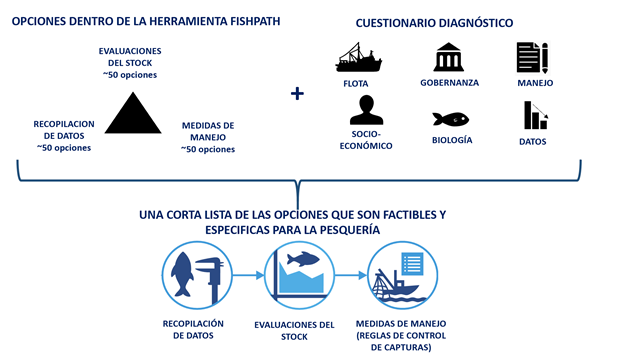
\includegraphics[width=0.75\linewidth]{images/fishpath-tool-overview-diagram-es} 

}

\caption{La herramienta FishPath a simple vista.}\label{fig:overview}
\end{figure}

\hypertarget{propuxf3sito-y-la-audiencia-de-la-guuxeda-de-uso-para-la-herramienta-fishpath}{%
\section{Propósito y la audiencia de la guía de uso para la herramienta FishPath}\label{propuxf3sito-y-la-audiencia-de-la-guuxeda-de-uso-para-la-herramienta-fishpath}}

La herramienta FishPath pretende ser utilizada en dos situaciones clave. La primera situacion es con un facilitador capacitado en el uso de la herramienta FishPath y la segunda es como usuario individual. Cada una de estas audiencias puede tener distintos niveles de experiencia y conocimiento en ciencias pesqueras y manejo.

\hypertarget{i.-uso-de-la-herramienta-en-un-proceso-liderado-por-un-facilitador-o-en-un-taller}{%
\subsubsection{I. Uso de la herramienta en un proceso liderado por un facilitador o en un taller:}\label{i.-uso-de-la-herramienta-en-un-proceso-liderado-por-un-facilitador-o-en-un-taller}}

La herramienta de FishPath está diseñada para ser navegada por científicos pesqueros capacitados en el uso de la misma, que puedan facilitar su aplicación con grupos de actores y usuarios relevantes a la pesquería. Estos usuarios pueden ser grupos multiactor (ej. científicos, manejadores, universidades, industria pesquera,) o usuarios de un solo sector (ej. agencia pesquera). El facilitador lidera la discusión alrededor del cuestionario y sus posibles respuestas. En este contexto, el facilitador con el uso de la herramienta FishPath busca abordar cualquier brecha de conocimiento relacionada con términos técnicos y conceptos presentados en la herramienta, mejorando la accesibilidad de los usuarios. En este caso, los miembros de la audiencia son expertos en la pesquería (incluyendo pescadores) y están familiarizados con las ciencias pesqueras y el manejo, pero no requieren ser expertos en ciencias pesqueras o en el aspecto cuantitativo del manejo pesquero.

\hypertarget{ii.-uso-de-la-herramienta-por-un-usuario-individual}{%
\subsubsection{II. Uso de la herramienta por un usuario individual:}\label{ii.-uso-de-la-herramienta-por-un-usuario-individual}}

La herramienta FishPath también tiene como intención ser usada por individuos o grupos sin el apoyo de un facilitador capacitado en FishPath (también referidos como ``usuarios de computadora'' o esos usuarios que utilizan la herramienta por su cuenta). Estos individuos tienen un conocimiento intermedio a avanzado en ciencias pesqueras y manejo. Para entender la herramienta en su totalidad y aplicarla de manera apropiada, se recomienda que estos usuarios lean y entiendan la guía de uso de la herramienta FishPath. Algunos ejemplos de usuarios individuales son:

\begin{itemize}
\tightlist
\item
  Científicos pesqueros, manejadores, estudiantes u otros profesionales de las pesquerías interesados en identificar opciones de evaluación apropiadas para pesquerías con datos limitados;
\item
  Científicos pesqueros, investigadores, o estudiantes que están interesados en revisar y comparar los componentes de una estrategia de capturas existente, contra las recomendaciones provistas por FishPath;
\item
  Científicos pesqueros, manejadores, estudiantes u otros profesionales que buscan material de referencia o una librería con material relacionado al manejo de pesquerías con datos limitados.
\end{itemize}

El propósito de la guía de usuario es explicar la funcionalidad de la herramienta y proveer instrucciones sobre cómo usar la herramienta de FishPath para seleccionar y revisar las mejores opciones para la colecta de datos, evaluaciones de stock, y medidas de manejo.

\hypertarget{iniciar-la-herramienta-fishpath}{%
\chapter{Iniciar la herramienta FishPath}\label{iniciar-la-herramienta-fishpath}}

Es importante notar que la herramienta FishPath requiere una conexión al internet constante para poder acceder al cuestionario, guardar las respuestas e interactuar con los resultados.

\hypertarget{puxe1gina-de-bienvenida}{%
\section{Página de Bienvenida}\label{puxe1gina-de-bienvenida}}

Cuando un usuario navega la página \url{https://www.tool.fishpath.org/}, aparece un mensaje de bienvenida con dos opciones: ``Crear cuenta'' o `` Iniciar sesión'' (Figura \ref{fig:welcome}).

\begin{figure}

{\centering 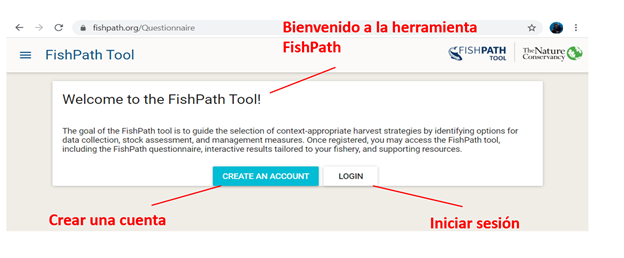
\includegraphics[width=0.95\linewidth]{images/welcome-page-es} 

}

\caption{Página de bienvenida para la herramienta FishPath y su traducción al español }\label{fig:welcome}
\end{figure}

\hypertarget{crear-una-cuenta-fishpath}{%
\section{Crear una cuenta FishPath}\label{crear-una-cuenta-fishpath}}

Al seleccionar ``Crear una cuenta'' (o ``Create an account''), una ventana aparecerá solicitando la siguiente información (Figura \ref{fig:create-account}). Un asterisco denota la información que es obligatoria proveer.

\begin{itemize}
\tightlist
\item
  Correo electrónico*
\item
  Contraseña* (Debe crear una contraseña)
\item
  Tipo de organización a la que pertenece*
\item
  Organización
\item
  Su nombre*
\item
  País de origen*
\end{itemize}

Es importante recordar que al ingresar su correo electrónico y su contraseña debe asegurar que utiliza adecuadamente letras mayúsculas y/o minúsculas.

Esta información será utilizada para poder rastrear el origen y el uso de la herramienta FishPath. Durante el paso de creación de la cuenta, también se indicará al usuario leer y aceptar los términos de servicio de la herramienta FishPath, elaborados por The Nature Conservancy (\protect\hyperlink{terms}{Appendix B}).

\begin{figure}

{\centering 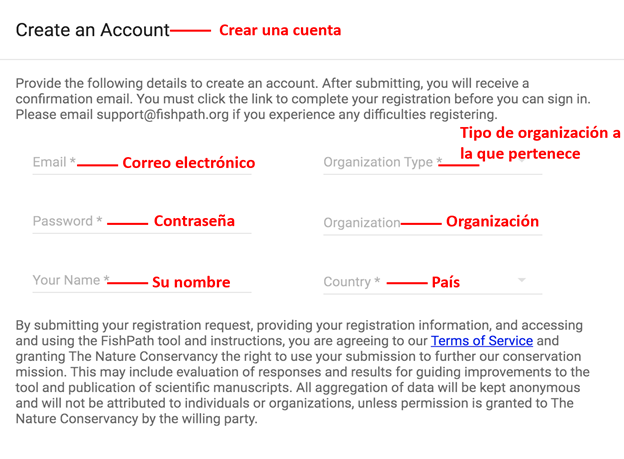
\includegraphics[width=0.95\linewidth]{images/create-account-es} 

}

\caption{Pantalla de “Crear una cuenta” de la herramienta FishPath}\label{fig:create-account}
\end{figure}

Despues de enviar una solicitud de cuenta, el usuario recibirá un correo de confirmación con un vínculo para completar el registro de su cuenta. Después de la creación de su cuenta, el usuario puede retornar cuando quiera a la página de Bienvenida en la herramienta FishPath al iniciar la sesión ingresando su correo y contraseña (Figura \ref{fig:login-page}).

\begin{figure}

{\centering 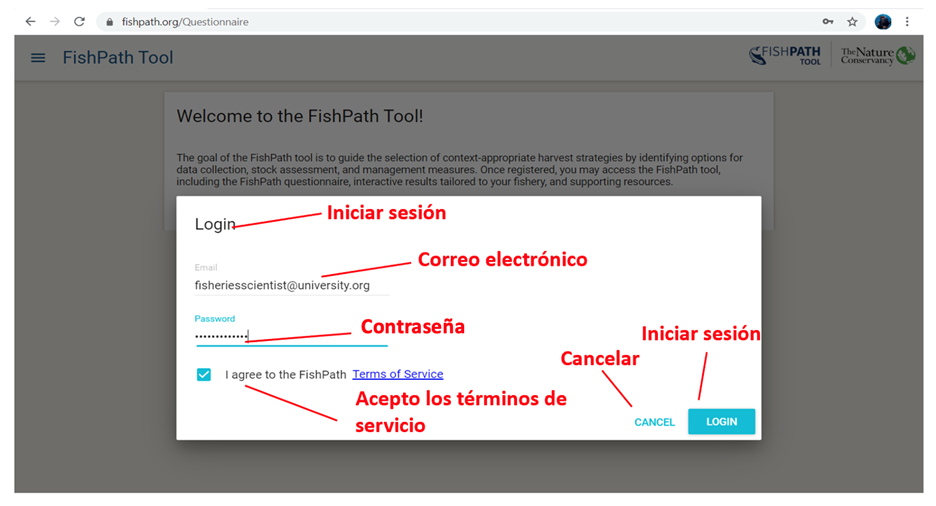
\includegraphics[width=0.95\linewidth]{images/login-page-es} 

}

\caption{Login Page of the FishPath Tool.}\label{fig:login-page}
\end{figure}

\hypertarget{tablero-de-la-herramienta-fishpath}{%
\section{Tablero de la herramienta FishPath}\label{tablero-de-la-herramienta-fishpath}}

Después de crear una cuenta (nuevo usuario) o de iniciar sesión (usuario existente), el usuario es dirigido al tablero o la ``página principal'' de la herramienta FishPath (Figura \ref{fig:dashboard}). En este tablero/página los usuarios ven 4 encabezados:

\begin{enumerate}
\def\labelenumi{\arabic{enumi}.}
\tightlist
\item
  \textbf{``Guía de uso de la herramienta FishPath''} el cual contiene todos los detalles para utilizar la herramienta FishPath e interpretación de los resultados.
\item
  \textbf{``Mis pesquerías''}, en donde se enlistan las pesquerías que el usuario ha iniciado o completado dentro de la herramienta. Usuarios pueden acceder a sus pesquerías en cualquier momento y pueden retornar a cuestionarios que se encuentren en progreso o a la página de los resultados.
\item
  \textbf{``Materiales de referencia''}, el cual provee una lista de todas las opciones disponibles en la herramienta FishPath con detalles y materiales de referencia a las mismas y en donde se puede descargar la lista de preguntas.
\item
  \textbf{``4. Obtener apoyo, hacer una pregunta o ayudar a mejorar la herramienta FishPath''}, que permite al usuario enviar preguntas o sugerencias al equipo FishPath.
\end{enumerate}

\begin{figure}

{\centering 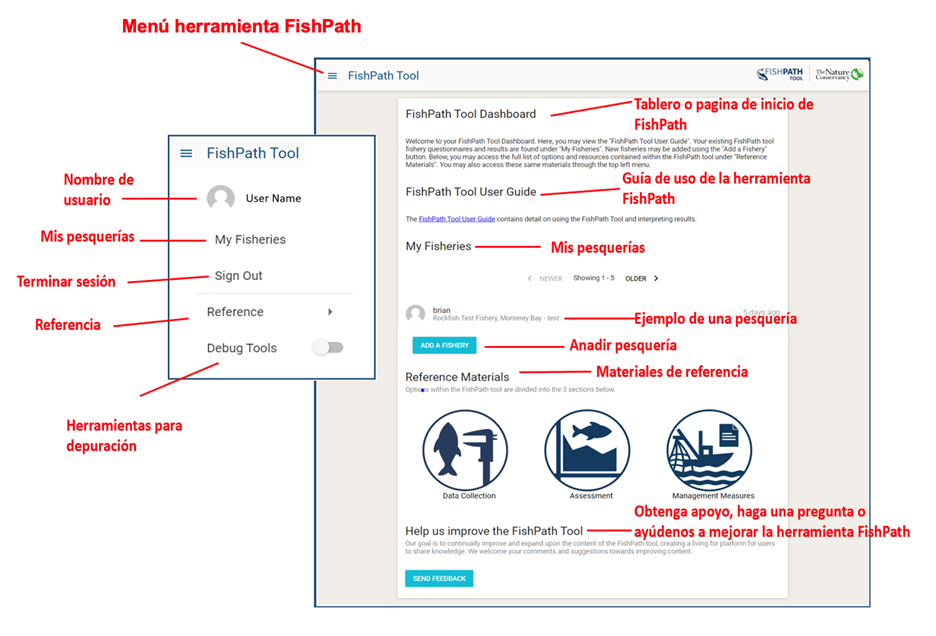
\includegraphics[width=0.95\linewidth]{images/user-dashboard-es} 

}

\caption{El tablero de la herramienta FishPath o la página principal para los usuarios que muestra los 4 encabezados descritos anteriormente. De la misma manera, al seleccionar la opción “Menú herramienta FishPath” (o “FishPath Tool”) en la esquina superior izquierda, se despliega un menú que permite al usuario navegar una serie de opciones.}\label{fig:dashboard}
\end{figure}

\hypertarget{menuxfa-herramienta-fishpath}{%
\subsubsection{Menú Herramienta FishPath}\label{menuxfa-herramienta-fishpath}}

En el lado superior izquierdo de la pantalla, los usuarios pueden ver una opción que dice ``Menú herramienta FishPath'' (o ``FishPath Tool'') y al hacer click en las 3 líneas horizontales aparece una ventana emergente con un menú. Este menú permite al usuario poder regresar al tablero, poder salir de su cuenta, acceder materiales de referencia y poder habilitar una opción llamada ``Saving status toolbar''.

Esta opción notificará al usuario sobre el estatus de su cuestionario, respuestas y resultados (Figura \ref{fig:saving-status}). Este barra de herramientas aparece abajo de la pantalla del cuestionario y le dice al usuario si sus respuestas han sido guardadas. Si las respuestas han sido guardadas, el texto mostrará ``All changes saved''. En el case de que no tenga buen internet, es posible que las respuestas no se guarden e inmediatamente va a aparecer una notificación en rojo indicando que no se han guardado los cambios o ``Changes pending'' mientras la herramienta continua tratando de guardar. Los usuarios no deben cerrar o refrescar el servidor hasta que las respuestas hayan sido guardadas, de lo contrario, es probable que los cambios no se guarden y se pierda su progreso. Para mayor información sobre cómo usar la herramienta en contextos de conectividad limitada, por favor revise \protect\hyperlink{faq-internet}{este sección de preguntas FAQ abajo}.

\begin{figure}

{\centering 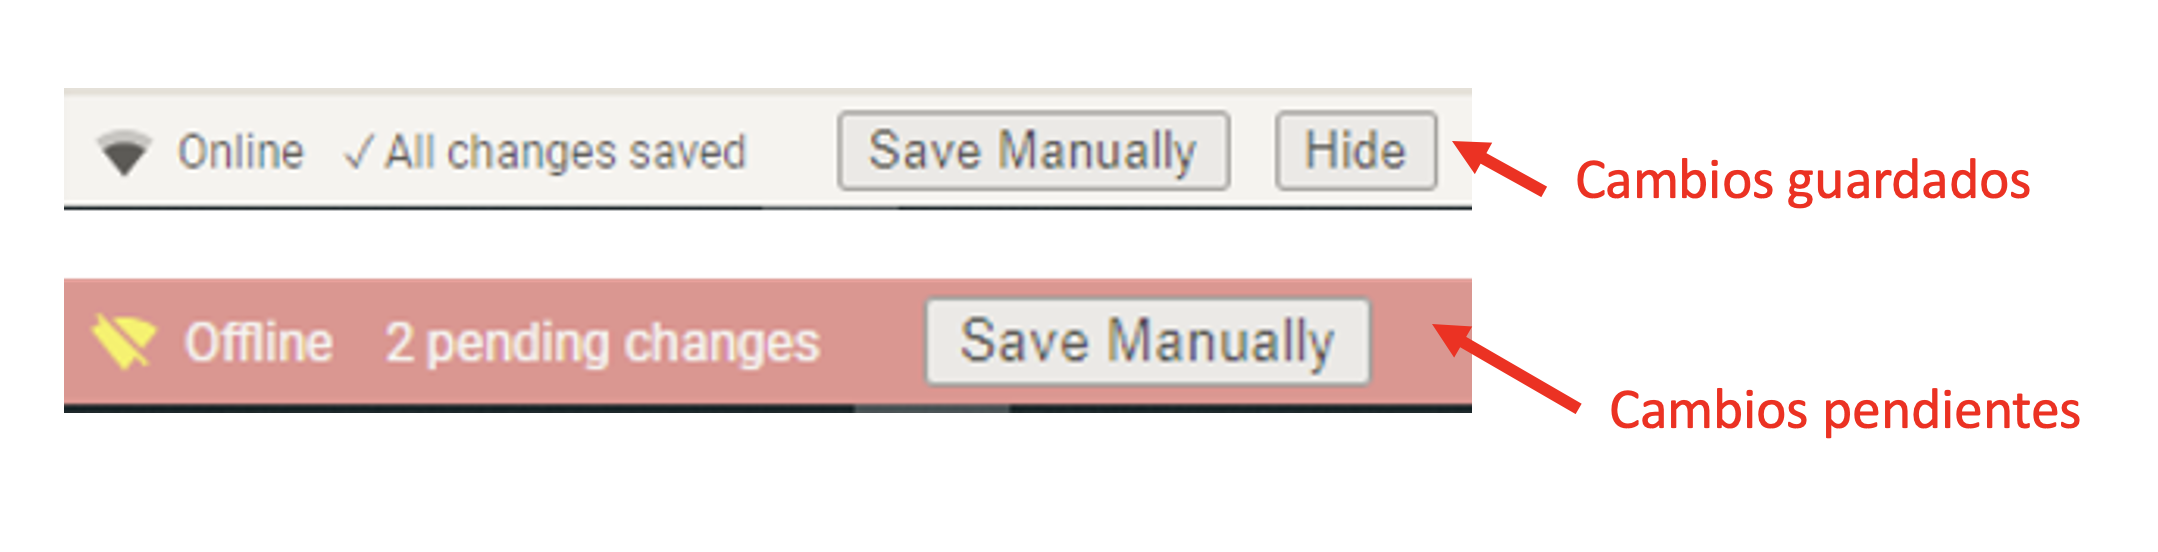
\includegraphics[width=0.95\linewidth]{images/saving-status-toolbar-es} 

}

\caption{Funcionalidad de la barra de herramientas del estado de guardado. La imagen superior muestra información o cambios guardados; la imagen inferior muestra cambios pendientes.}\label{fig:saving-status}
\end{figure}

\hypertarget{auxf1adir-una-pesqueruxeda}{%
\section{Añadir una pesquería}\label{auxf1adir-una-pesqueruxeda}}

Al seleccionar el botón azul de ``Añadir una pesquería'' el usuario podrá empezar una pesquería nueva en la herramienta FishPath que será añadida a su cuenta. Primero, una ventana aparecerá llamada ``Información sobre la pesquería'', la cual dará lugar a los usuarios a definir aspectos generales de la pesquería de interés (Figura \ref{fig:fishery-info}), usando los campos que se proveen a continuación. Esta información ayuda a los usuarios a definir mejor la pesquría a la que aplicarán la herramienta FishPath, para que las respuestas sean dirigidas únicamente a esa pesquería de interés. Esta información también es útil para TNC para entender mejor el uso de la herramienta de FishPath y proveer información de alto nivel de las características de la pesquería.

Las pesquerías y la información guardada en la herramienta de FishPath (incluyendo respuestas, notas y resultados) es accesible únicamante para los usuarios que ingresaron los datos y para los administradores de la herramienta FishPath. Si el usuario desea, puede \protect\hyperlink{Results-Actions}{\textbf{compartir sus resultados}} con otros usuarios.

\begin{itemize}
\tightlist
\item
  Nombre común de la pesquería
\item
  Género y especie
\item
  Flota y tipos de arte de pesca
\item
  País o Países
\item
  Área geográfica de la pesquería
\item
  En cuál de estos 3 contextos es la herramienta FishPath siendo utilizada para esta pesquería?

  \begin{itemize}
  \tightlist
  \item
    Prueba exploratoria\\
  \item
    Taller facilitado para una pesquería especifica
  \item
    Uso individual para una pesquería especifica
  \end{itemize}
\end{itemize}

\begin{figure}

{\centering 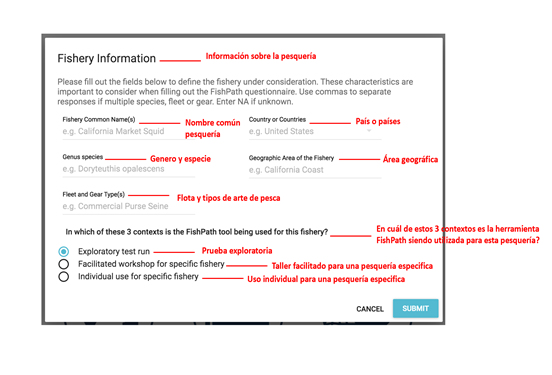
\includegraphics[width=0.95\linewidth]{images/fishery-info-screen-es} 

}

\caption{Campos de información que aparecen en la ventana llamada “Información sobre la pesquería”}\label{fig:fishery-info}
\end{figure}

Al seleccionar la opcion ``Ingresar'' (o ``Submit''), el usuario deberá seleccionar uno de los 3 componentes de la estrategia de capturas (secciones) de la herramienta FishPath (colecta de datos, evaluación del stock y medidas de manejo) y empezará el cuestionario de la herramienta FishPath. Los usuarios pueden completar y ver sus resultados de cualquiera de estas secciones de manera independiente. Un ícono de un lápiz en la esquina superior derecha permite al usuario editar la información de la pesquería en cualquier momento (Figura \ref{fig:fishery-entry}).

\begin{figure}

{\centering 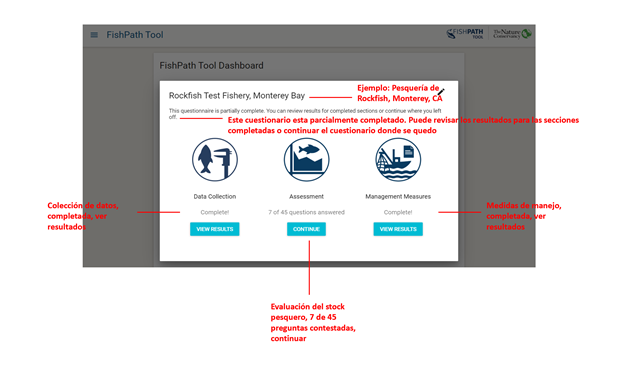
\includegraphics[width=0.95\linewidth]{images/fishery-entry-screen-es} 

}

\caption{Pantalla de entrada al cuestionario de la herramienta FishPath después que la información sobre la pesquería ha sido definida.}\label{fig:fishery-entry}
\end{figure}

\hypertarget{cuestionario-de-la-herramienta-fishpath}{%
\chapter{Cuestionario de la herramienta FishPath}\label{cuestionario-de-la-herramienta-fishpath}}

La meta del cuestionario de la herramienta FishPath es obtener información sobre todos los aspectos de la pesquería. Esta información conlleva a la activación de ciertos supuestos, precauciones y consideraciones a tener en cuenta para cada opción. A través de las tres secciones (colecta de datos, evaluación del stock y medidas de manejo) el usuario contesta alrededor de \textasciitilde120 preguntas. Las preguntas están divididas en 6 categorías, las cuales indican la naturaleza de la información que se busca:

\begin{enumerate}
\def\labelenumi{\arabic{enumi}.}
\tightlist
\item
  Biología/ ciclos biológicos y ecológicos de la especie
\item
  Disponibilidad de datos
\item
  Gobernanza
\item
  Manejo
\item
  Características operacionales
\item
  Características socioeconómicas
\end{enumerate}

Algunas preguntas son relevantes para múltiples secciones (colecta de datos, evaluación y medidas de manejo). Una vez que hayan sido contestadas, estas no van a aparecer en otras secciones subsecuentes. Para más información sobre cómo se muestran las preguntas que abarcan varias secciones, consulte estas \protect\hyperlink{faq-question-numbering}{preguntas frecuentes a continuación}.

En cualquier momento, el usuario puede cerrar sesión y retornar a la misma a través de la opción ``Mis pesquerías'' en la página de Inicio o tablero de la herramienta. Una vez que el usuario haya completado una sección, se puede revisar los resultados o puede continuar con la siguiente sección. Los resultados de las secciones se hacen disponibles una vez que el usuario completa todas las preguntas del respectivo cuestionario.

Después de revisar la página de entrada al cuestionario FishPath (Figura \ref{fig:fishery-entry}), el usuario debe seleccionar una de las 3 secciones. Debajo del nombre de cada sección, se mostrará el número de preguntas dentro de dicha sección y un párrafo que explica cómo contestar las preguntas (Figura \ref{fig:dc-overview}). El usuario puede elegir la opción de ``Comenzar'' (``Begin'') la sección o ``Elegir otra sección'' (``Choose Another Section'').

\begin{figure}

{\centering 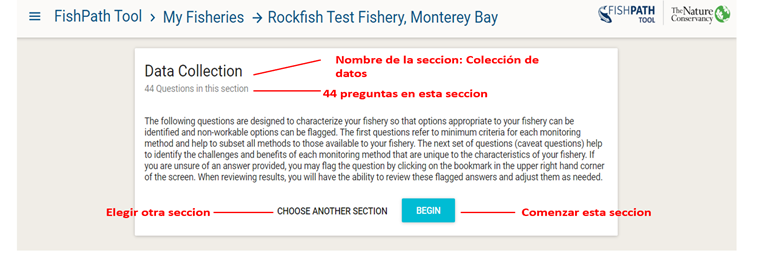
\includegraphics[width=0.95\linewidth]{images/dc-overview-es} 

}

\caption{Visión general de la sección colecta de datos}\label{fig:dc-overview}
\end{figure}

\hypertarget{anatomuxeda-de-una-pregunta-dentro-de-la-herramienta-fishpath}{%
\section{Anatomía de una pregunta dentro de la herramienta FishPath}\label{anatomuxeda-de-una-pregunta-dentro-de-la-herramienta-fishpath}}

La figura \ref{fig:question-anatomy} y la figura \ref{fig:bookmark-notes} provee un ejemplo de lo que se observa en la pantalla cuando se quiere contestar una pregunta dentro de la herramienta:

\begin{figure}
 
 {\centering 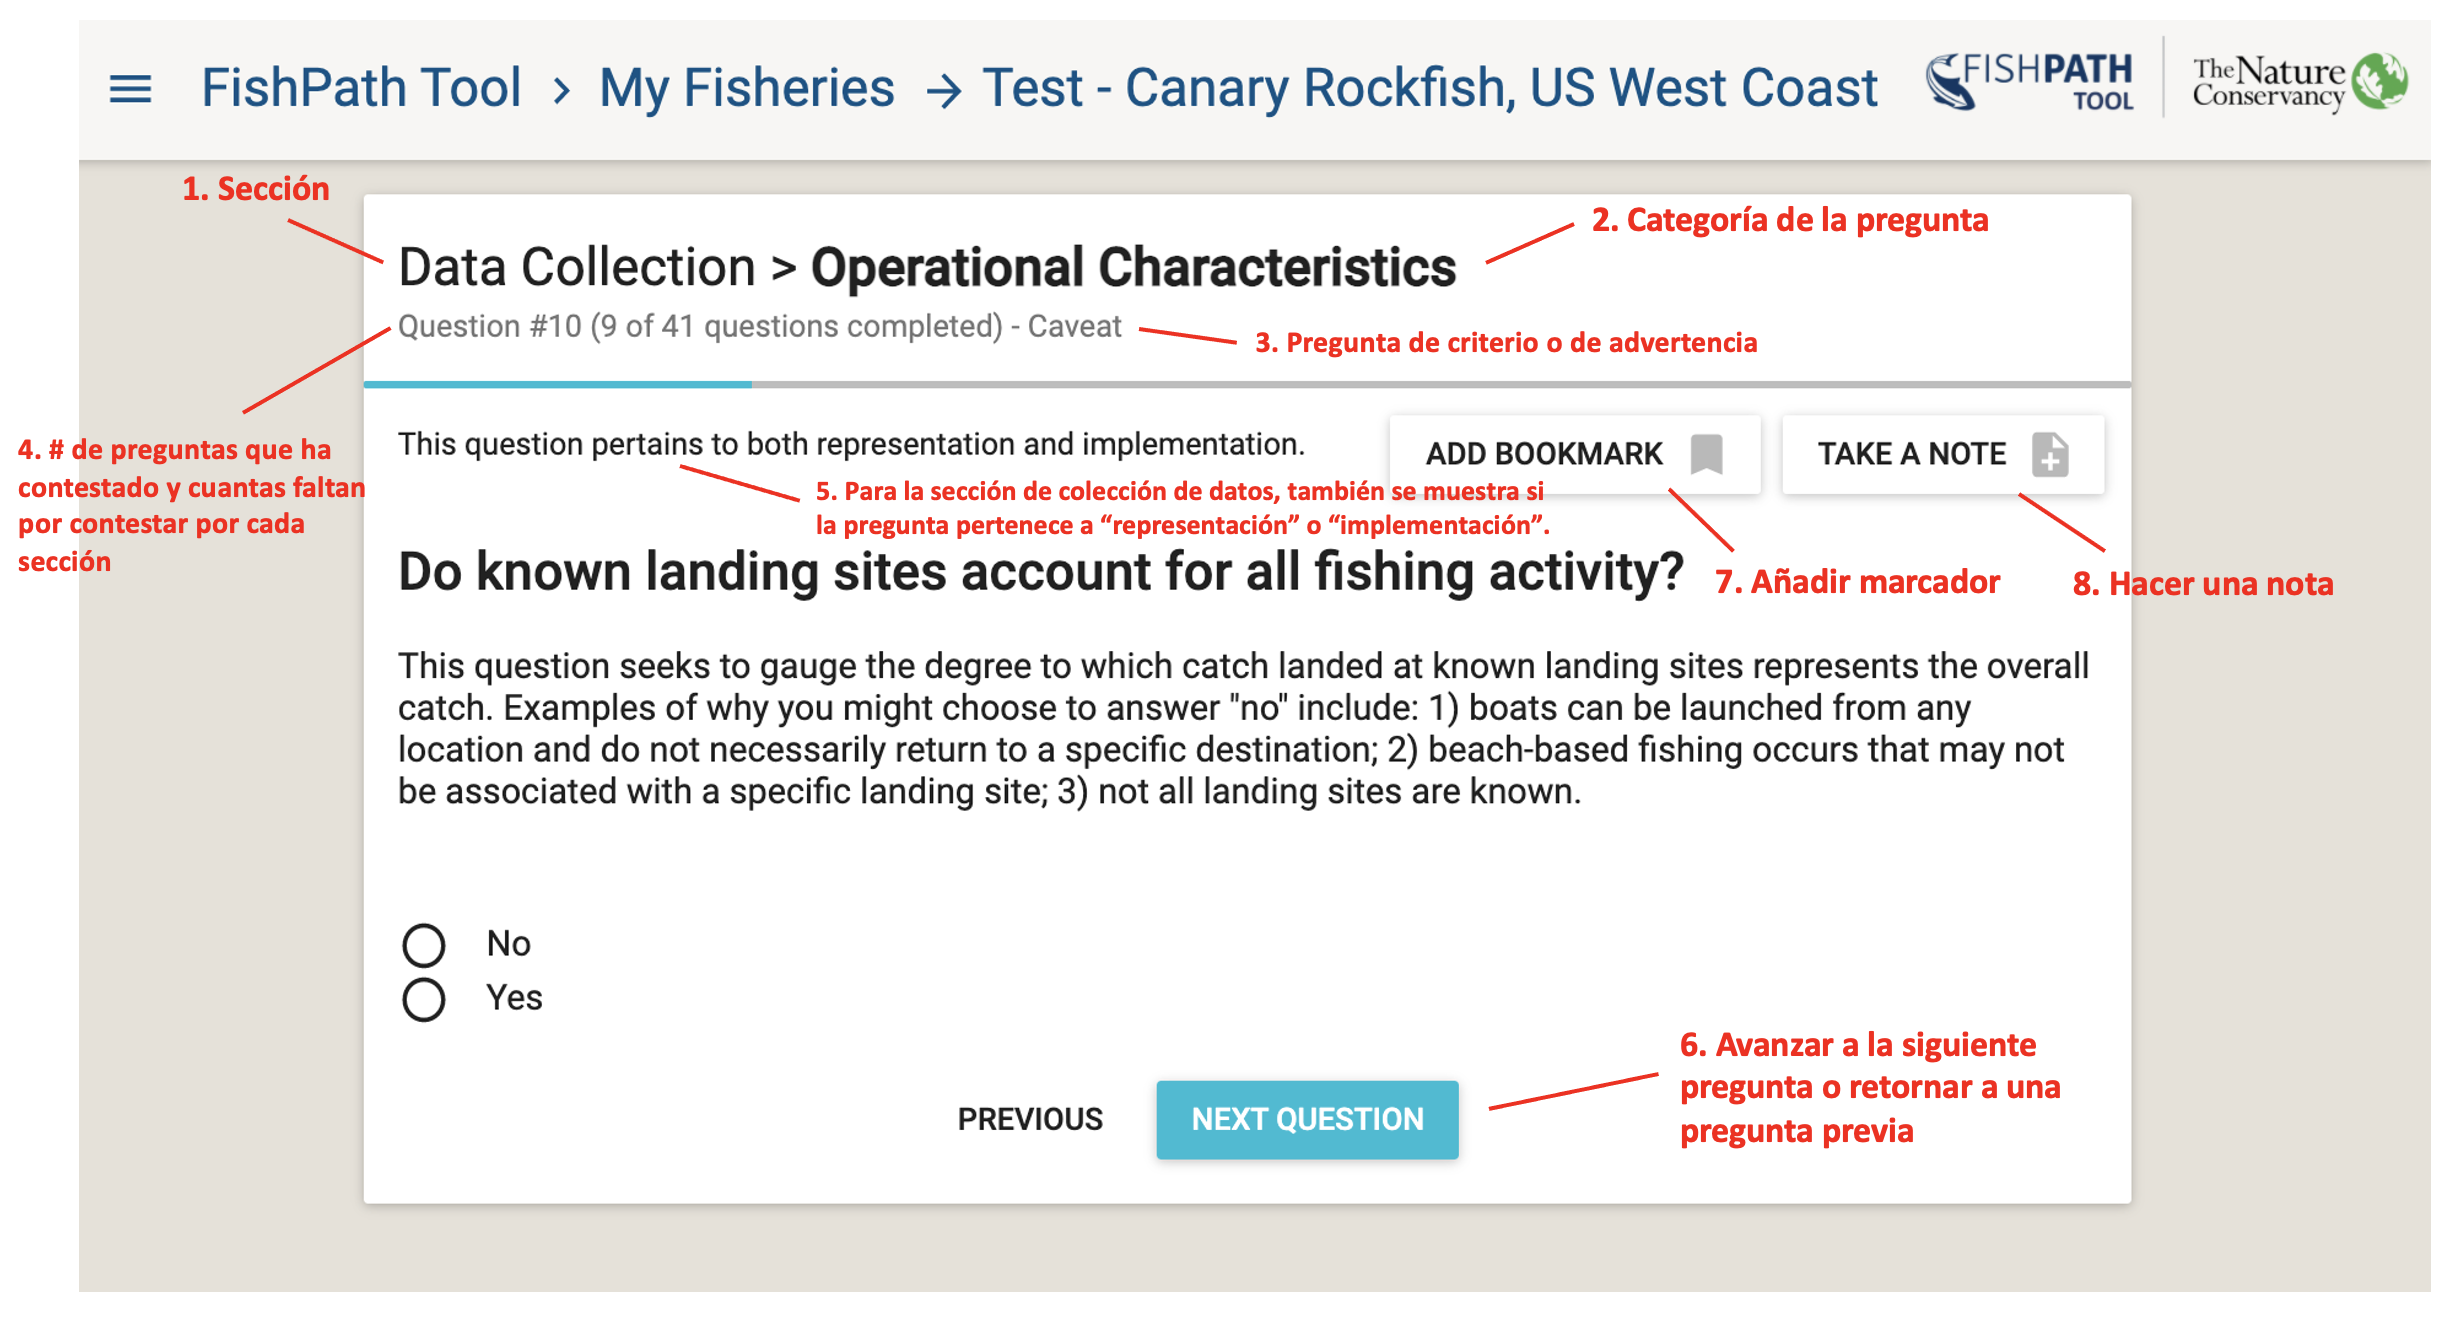
\includegraphics[width=0.95\linewidth]{images/question-anatomy-es} 
 
 }
 
 \caption{Anatomia de una pregunta dentro de la herramienta FishPath.}\label{fig:question-anatomy}
 \end{figure}

\begin{enumerate}
\def\labelenumi{\arabic{enumi}.}
\tightlist
\item
  En la parte superior de la pantalla, se muestra la \textbf{sección}: colecta de datos, evaluación del stock o medidas de manejo.
\item
  Al lado de la sección, se muestra la \textbf{categoría de cada pregunta} (i.e., Biología/historia de vida, Disponibilidad de datos, Gobernanza, Manejo, Características Operacionales o Características socioeconómicas).
\item
  Debajo del nombre de la sección y categoría de cada pregunta, se muestra un pequeño encabezado que muestra si la pregunta es de \textbf{``criterio'' o de ``advertencia''}.
\item
  Este encabezado muestra el \textbf{número de preguntas que ha contestado} y cuantas faltan por contestar dentro de esa sección.
\item
  Para la sección ``Colecta de datos'', también se muestra si la pregunta es de ``representación'' o ``implementación''. Esto indica al usuario si la pregunta tiene implicaciones en la habilidad de colectar datos representativos o de implementar un programa de colecta de datos, o ambos. La intención es ayudar al usuario a entender y responder de mejor manera la pregunta.
\item
  Abajo de la pantalla, el usuario puede avanzar a \textbf{la próxima pregunta (o ``Next Question'')} o retornar a \textbf{la pregunta anterior (o ``Previous'')}.
\item
  Hay una opción de \textbf{``Marca la pregunta'' (o ``Bookmark'')}. Al marcar ciertas preguntas da facilidad al usuario de poder revisarlas posteriormente (Figura \ref{fig:bookmark-notes}). Una pregunta puede ser marcada por distintas razones, tales como: desconocimiento sobre la respuesta, necesita mayor discusión para llegar a un acuerdo, se necesita consultar cierta información, el usuario considera que la pregunta es crítica, etc. Como todas las preguntas deben ser contestadas para revisar los resultados, añadir un marcador permite al usuario proveer una respuesta temporal que puede ser revisada y modificada en la sección de resultados, una vez que el usuario pueda evaluar el impacto relativo de dicha respuesta.
\item
  Los usuarios pueden \textbf{``hacer una nota'' (o ``Take a Note'')} en cualquier pregunta (Figura \ref{fig:bookmark-notes}). Las notas también sirven para múltiples razones, como clarificar porqué cierta respuesta fue dada, capturar una discusión importante , indicar que se necesita investigar más antes de responder, etc. Posteriormente, las notas pueden formar parte de un borrador para el desarrollo de una estrategia de capturas y al proveer justificación a respuestas, se tendrá replicabilidad y trazabilidad. Al estar conectado al internet, todas las notas serán guardadas dentro de la herramienta FishPath y podrán ser utilizadas como referencia por el usuario.
\end{enumerate}

\begin{figure}
 
 {\centering 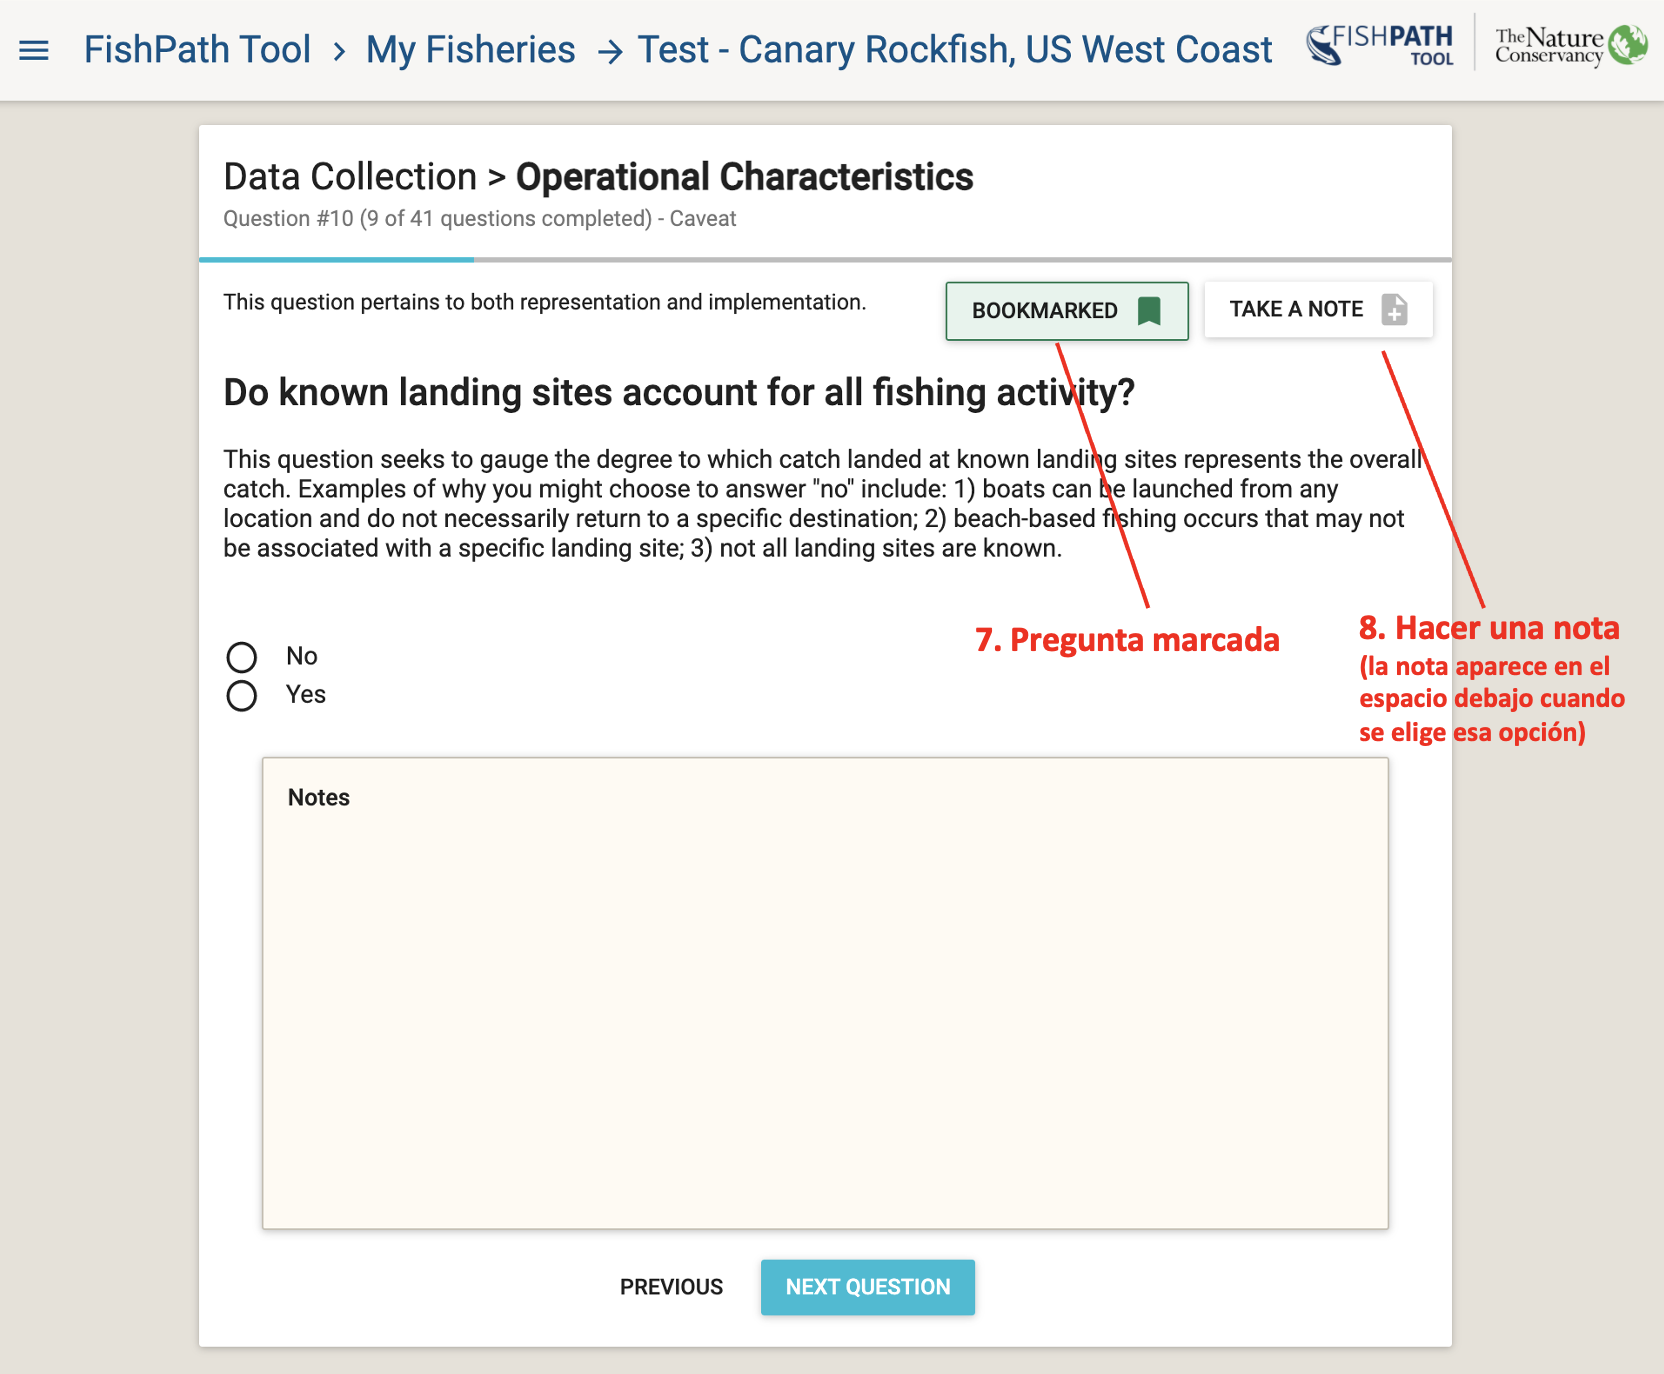
\includegraphics[width=0.95\linewidth]{images/bookmark-notes-es} 
 
 }
 
 \caption{Ejemplo de una pregunta dentro de la herramienta FishPath con la pregunta marcada (en verde) y la nota agregada (caja de texto).}\label{fig:bookmark-notes}
 \end{figure}

\hypertarget{preguntas-de-criterio-o-advertencia}{%
\section{Preguntas de ``Criterio'' o ``Advertencia''}\label{preguntas-de-criterio-o-advertencia}}

Las preguntas se designan como ``criterio'' o ``advertencia'' o ambos, lo cual se refiere a cómo las respuestas se vinculan a las preguntas contenidas dentro de la herramienta.

Una pregunta de criterio determina si la pesquería cumple con la mínima calificación requerida para aplicar una opción. Preguntas cuyas respuestas invoquen ``advertencias'' no van a eliminar o retener opciones, pero van a invocar advertencias de colores (rojo, amarillo, anaranjado) o atributos positivos (verdes) contra opciones específicas.

\hypertarget{preguntas-subjetivas}{%
\section{Preguntas subjetivas}\label{preguntas-subjetivas}}

Mientras que la mayoría de las preguntas en la herrameinta FishPath se pueden contestar definitva y objetivamente, también hay ciertas preguntas subjetivas por su naturaleza. Por ejemplo, una pregunta subjetiva puede requerir que se clasifiquen ciertas caracetrísticas de la pesquería en una escala (ejemplo: bajo, medio y alto). Este diseño subjetivo es intencional, ya que permite a los usuarios pensar en características clave, relativas a su pesquería que van a impactar la viabilidad de implementar ciertas opciones de manejo.

Generalmente, el mejor enfoque al completar el cuestionario es hacerlo de manera eficaz, sin perder mucho tiempo en debatir sobre ciertas preguntas. Cuando se tenga una duda, la pregunta puede ser marcada, o se pueden tomar notas, para poder revisar la pregunta posteriormente. La transparencia de la herramienta FishPath es tal que los usuarios pueden ver como su respuesta a cualquier pregunta impacta los resultados (por medio de los criterios y consideraciones) y que los usuarios pueden \protect\hyperlink{Bookmark-Influential}{\textbf{cambiar su respuesta si así lo desean}}. Además, el objetivo del cuestionario es el de obtener un vistazo general de las características de la pesquería, para poder informar mejor las opciones de la estrategia de capturas. Como tal, las preguntas pueden impactar a pocas opciones o puede que no invoquen fuertes advertencias. El objetivo es apreciar la pesquería en su totalidad, más que enfocarse a una sola pregunta.

\hypertarget{completar-el-cuestionario}{%
\section{Completar el cuestionario}\label{completar-el-cuestionario}}

Al completar o salir de cualquiera de las tres secciones, aparecerá una ventana indicando el estado o progreso del cuestionario (Figura \ref{fig:summary-screen}). Los usuarios podrán revisar los resultados para aquellas secciones completadas o de otra manera, continuar con el cuestionario.

El cuestionario de FishPath se revisa periódicamente para reflejar la ciencia pesquera más actualizada. En caso de haber preguntas nuevas o pendientes, la sección no se mostrará como ``Completa'', en la ventana emergente del resumen al regresar al cuestionario de la pesquería (Figura \ref{fig:summary-screen}). En su lugar, se mostrará el número de preguntas respondidas del número total de preguntas (por ej., ``45 de 46 preguntas respondidas''). Para obtener mayor información sobre las actualizaciones del cuestionario, consulte \protect\hyperlink{faq-content-updates}{estas preguntas frecuentes a continuación}.

\begin{figure}
 
 {\centering 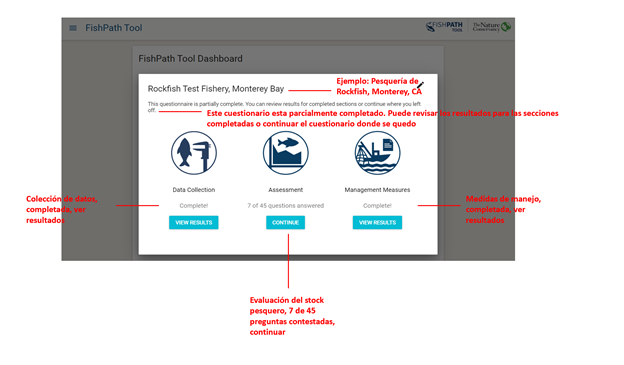
\includegraphics[width=0.95\linewidth]{images/summary-screen-es} 
 
 }
 
 \caption{Ventana con el resumen de las 3 secciones del cuestionario FishPath, demostrando el progreso del cuestionario.}\label{fig:summary-screen}
 \end{figure}

\hypertarget{marco-conceptual-de-la-herramienta-fishpath}{%
\section{Marco conceptual de la herramienta FishPath}\label{marco-conceptual-de-la-herramienta-fishpath}}

En un panorama general, la herramienta FishPath es un marco conceptual que combina las respuestas del usuario al cuestionario con más 150 opciones contenidas dentro de la herramienta (Figure \ref{fig:conceptual}). En otras palabras, las respuestas de los usuarios a las preguntas ayudan a caracterizar la pesquería. Cada respuesta puede disparar consideraciones cuando se aplica una opción a la pesquería. Estas consideraciones (y tipos de preguntas) pueden tomar dos formas. Los criterios denotan que la pesquería cumple o no cumple con los requerimientos básicos para poder usar cierta opción. Alternativamente, las advertencias se clasifican según su intensidad, en colores de semáforo, o advertencies estáticas que siempre aplican a la opción.

\begin{figure}
 
 {\centering 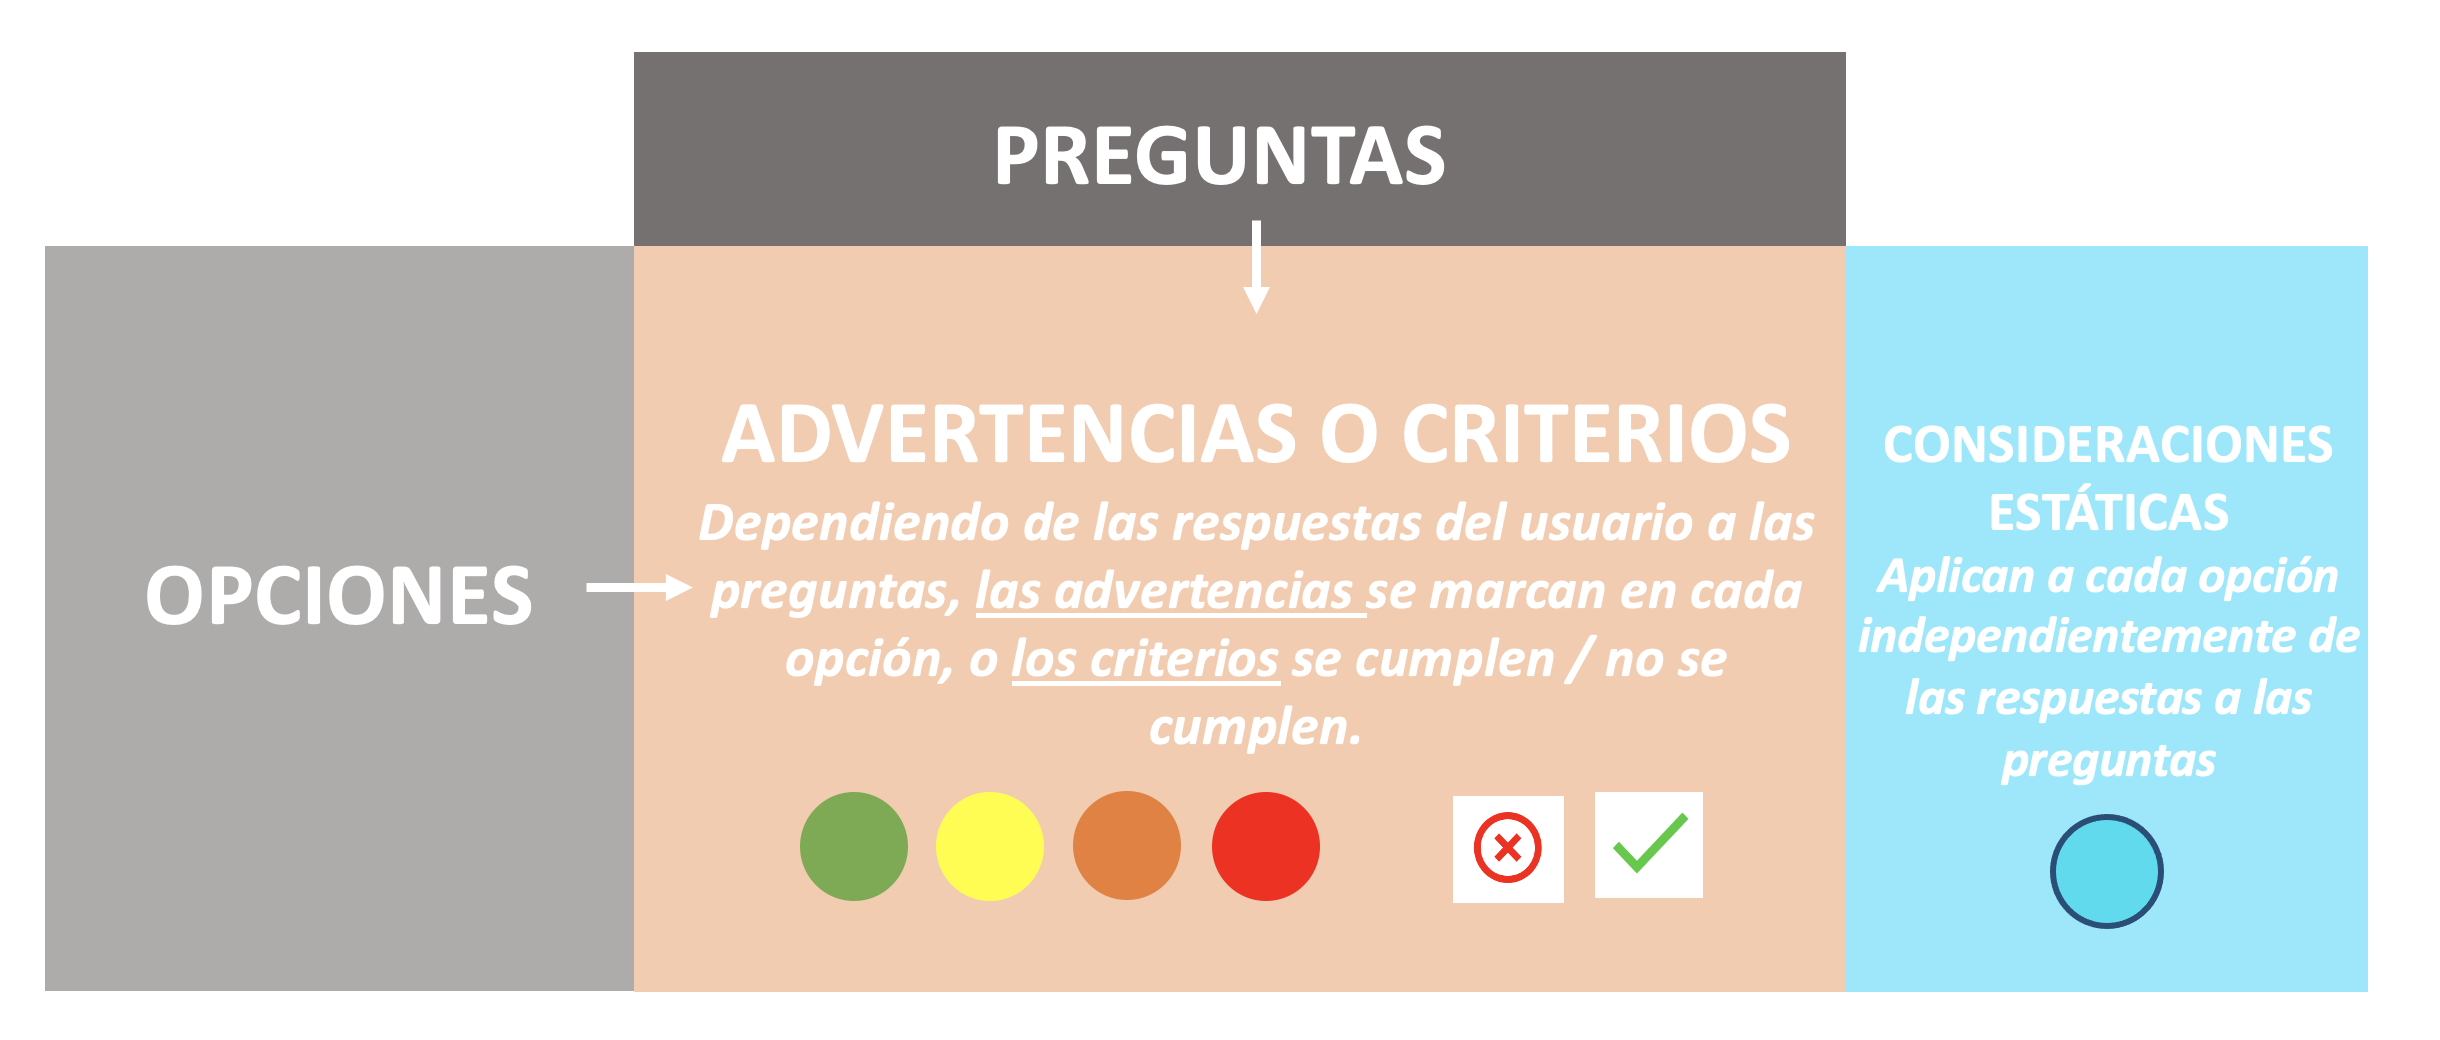
\includegraphics[width=0.95\linewidth]{images/conceptual-framework-es} 
 
 }
 
 \caption{Marco conceptual de la herramienta FishPath, que demuestra los vínculos entre preguntas, opciones, y criterios o advertencias.}\label{fig:conceptual}
 \end{figure}

\hypertarget{herramienta-fishpath-visiuxf3n-general-del-marco-conceptual-y-sus-3-secciones}{%
\subsection{Herramienta FishPath: Visión general del marco conceptual y sus 3 secciones}\label{herramienta-fishpath-visiuxf3n-general-del-marco-conceptual-y-sus-3-secciones}}

\hypertarget{secciuxf3n-de-colecta-de-datos}{%
\subsubsection{Sección de colecta de datos}\label{secciuxf3n-de-colecta-de-datos}}

La sección de colecta de datos busca apoyar al usuario en entender qué categorías generales de información colectar y los mecanismos para hacerlo, que sean óptimos para el contexto de la pesquería, las capacidades, y realidades para la implementación en sitio.

Existen diversas opciones para la colecta de datos (desde encuestas de mercados hasta bitácoras de pesca y programas de observadores a bordo). Estas opciones se subdivididen de acuerdo a la categoría general de información que puede ser colectada, ya que ésta influenciará la viabilidad de la opción para la colecta de datos. Las \protect\hyperlink{Data-Categories}{\textbf{cuatro categorías de datos}} en la herramienta FishPath son: 1) datos que arrojan un conocimiento básico de la pesquería; 2) información biológica; 3) datos que informan análisis de tendencias temporales (datos de series de tiempo); y 4) datos con calidad suficiente para poder informar una evaluación del stock.

\hypertarget{secciuxf3n-de-evaluaciones}{%
\subsubsection{Sección de evaluaciones}\label{secciuxf3n-de-evaluaciones}}

La sección de evaluaciones de stock permite al usuario entender los métodos disponibles y más apropiados para evaluar pesquerías con datos limitados. En la herramienta FishPath, una evaluación se define como cualquier análisis o indicador de desempeño que provee información, ya sea por medidas directas o indirectas del estado del stock, y que sea útil para el manejo. Esto puede variar desde ``motivo de preocupación'' proveniente de una opinión de un experto pesquero, análisis de riesgo cualitativas, valores empíricos de indicadores relativos a niveles predefinidos que desencadenan ciertos resultados, marco de indicadores múltiples, análisis de la historia de vida de la especie que proveen estimaciones de la mortalidad de pesca F, o la mortalidad de pesca cuando la pesquería se encuentra en su rendimiento máximo sostenible FMSY, modelos basados en capturas, modelos basados en tallas, hasta modelos de dinámica poblacional para estimar la biomasa.

Con base en las características de cada pesqueria y en la calidad y el tipo de datos disponibles (proveniente del cuestionario) el usuario marca advertencias y criterios contra las \protect\hyperlink{Assessment-Categories}{\textbf{opciones de evaluación del stock}}.

\hypertarget{secciuxf3n-de-medidas-de-manejo}{%
\subsubsection{Sección de medidas de manejo}\label{secciuxf3n-de-medidas-de-manejo}}

La sección de medidas de manejo permite al usuario revisar y filtrar las opciones apropiadas para manejar la mortalidad de la pesqueria. Las \protect\hyperlink{Management-Measure-Categories}{\textbf{opciones de medidas de manejo}} pueden tomar diversas formas incluyendo restricciones espaciales, temporales, de esfuerzo, de captura y de las artes de pesca. La herramienta FishPath no tiene criterios mínimos para las medidas de manejo pero utiliza advertencias. Múltiples medidas de manejo pueden y deberían de utilizarse en conjunto. La herramienta FishPath no es prescriptiva ni ofrece guianza en la forma específica de las reglas de cosecha, sin embargo, puede dirigir u orientar a los usuarios hacia recursos y herramientas que pueden apoyar este proceso, ubicados dentro de las descripciones de cada opción.

\hypertarget{puxe1gina-interactiva-de-resultados-de-la-herramienta-fishpath}{%
\chapter{Página interactiva de Resultados de la herramienta FishPath}\label{puxe1gina-interactiva-de-resultados-de-la-herramienta-fishpath}}

La página interactiva de resultados de la herramienta FishPath permite a los usuarios visualizar e interactuar con las opciones contenidas dentro de FishPath para poder entender como cada opción puede ser aplicable a su pesquería.

Al completar el cuestionario para cada sección, el usuario es dirigido a la página interactiva de resultados de la herramienta FishPath (Figura \ref{fig:results-overview}). Los resultados son presentados separadamente para cada una de las 3 secciones, o componente de la estrategia de capturas: 1) colecta de datos; 2) evaluación del stock; y 3) medidas de manejo (Figura \ref{fig:results-overview}, las secciones se muestran en azul oscuro, cerca del principio de la pantalla).

Se puede acceder a cada una de las tres secciones de resultados individualmente sin necesidad de completar las tres secciones. Si un usuario no ha completado el cuestionario por lo menos de una sección, serán dirigidos a completar el cuestionario de la sección antes de poder acceder a sus resultados (Figura \ref{fig:summary-screen}).

En esta sección los usuarios deben comenzar con el proceso ``Narrow your Results'' o reducir sus resultados (Figura \ref{fig:results-overview}, botón azul). Abajo, la funcionalidad y disposición de la pantalla es explicada, seguida por los pasos a seguir en el proceso de reducir las opciones de sus resultados.

\begin{figure}

{\centering 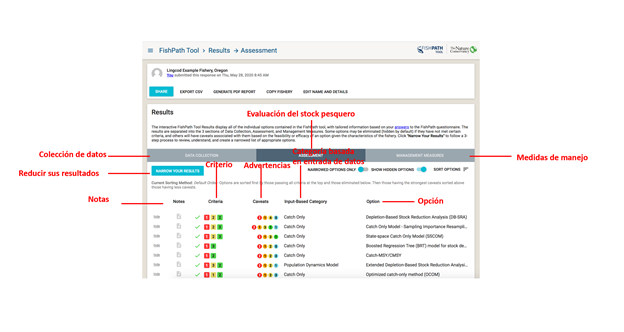
\includegraphics[width=0.95\linewidth]{images/results-overview-es} 

}

\caption{Resultados iniciales en la pantalla de resultados de la herramienta FishPath (en la imagen se muestra la sección de evaluaciones de stock), mostrando únicamente un extracto de los resultados, no de la lista completa.}\label{fig:results-overview}
\end{figure}

La figura \ref{fig:results-components} muestra los componentes generales de la página de resultados. Cada uno se detalla a continuación:

\begin{enumerate}
\def\labelenumi{\arabic{enumi}.}
\tightlist
\item
  \protect\hyperlink{interactive-results-table}{Tabla interactiva de resultados}
\item
  \protect\hyperlink{Filters-Sorting}{Mostrar opciones escondidas y ordenar opciones}
\item
  \protect\hyperlink{Bookmark-Influential}{Preguntas que han sido marcadas y respuestas influyentes}
\item
  \protect\hyperlink{Results-Narrowing}{Resultados del proceso de reducción de opciones}
\item
  \protect\hyperlink{Results-Actions}{Acciones para compartir resultados y editar información de la pesquería}
\item
  \protect\hyperlink{View-Only}{Modo de ver únicamente (para compartir la información de una pesquería)}
\end{enumerate}

\begin{figure}

{\centering 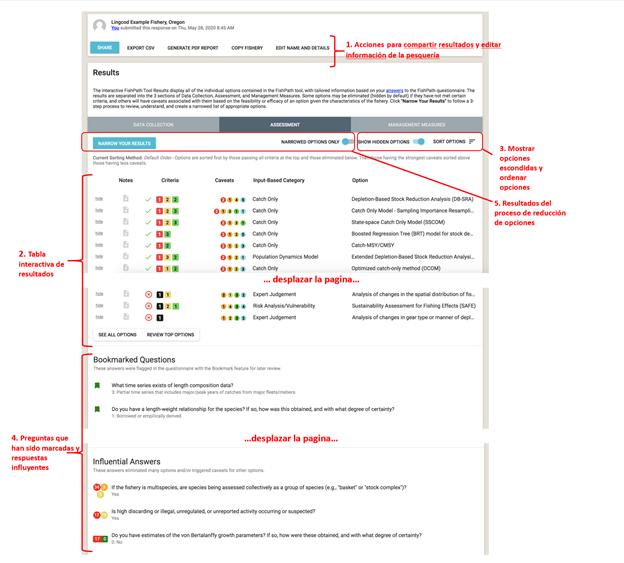
\includegraphics[width=0.95\linewidth]{images/results-components-es} 

}

\caption{Componentes clave (etiquetas en rojo del 1-5) de la pantalla interactiva de los resultados de la herramienta FishPath.}\label{fig:results-components}
\end{figure}

\hypertarget{interactive-results-table}{%
\section{Cuadro interactivo de resultados}\label{interactive-results-table}}

La lista de resultados contiene las opciones disponibles para esa sección. Cada fila representa una opcion (Figura \ref{fig:result-rows}) y resume qué criterio se cumplió o falló y qué advertencias surgieron, entre otros detalles. Cada opción puede ser seleccionada y expandida para ver su descripción y lista de criterios y advertencias. Cada componente de las filas se explica a continuación.

\begin{figure}

{\centering 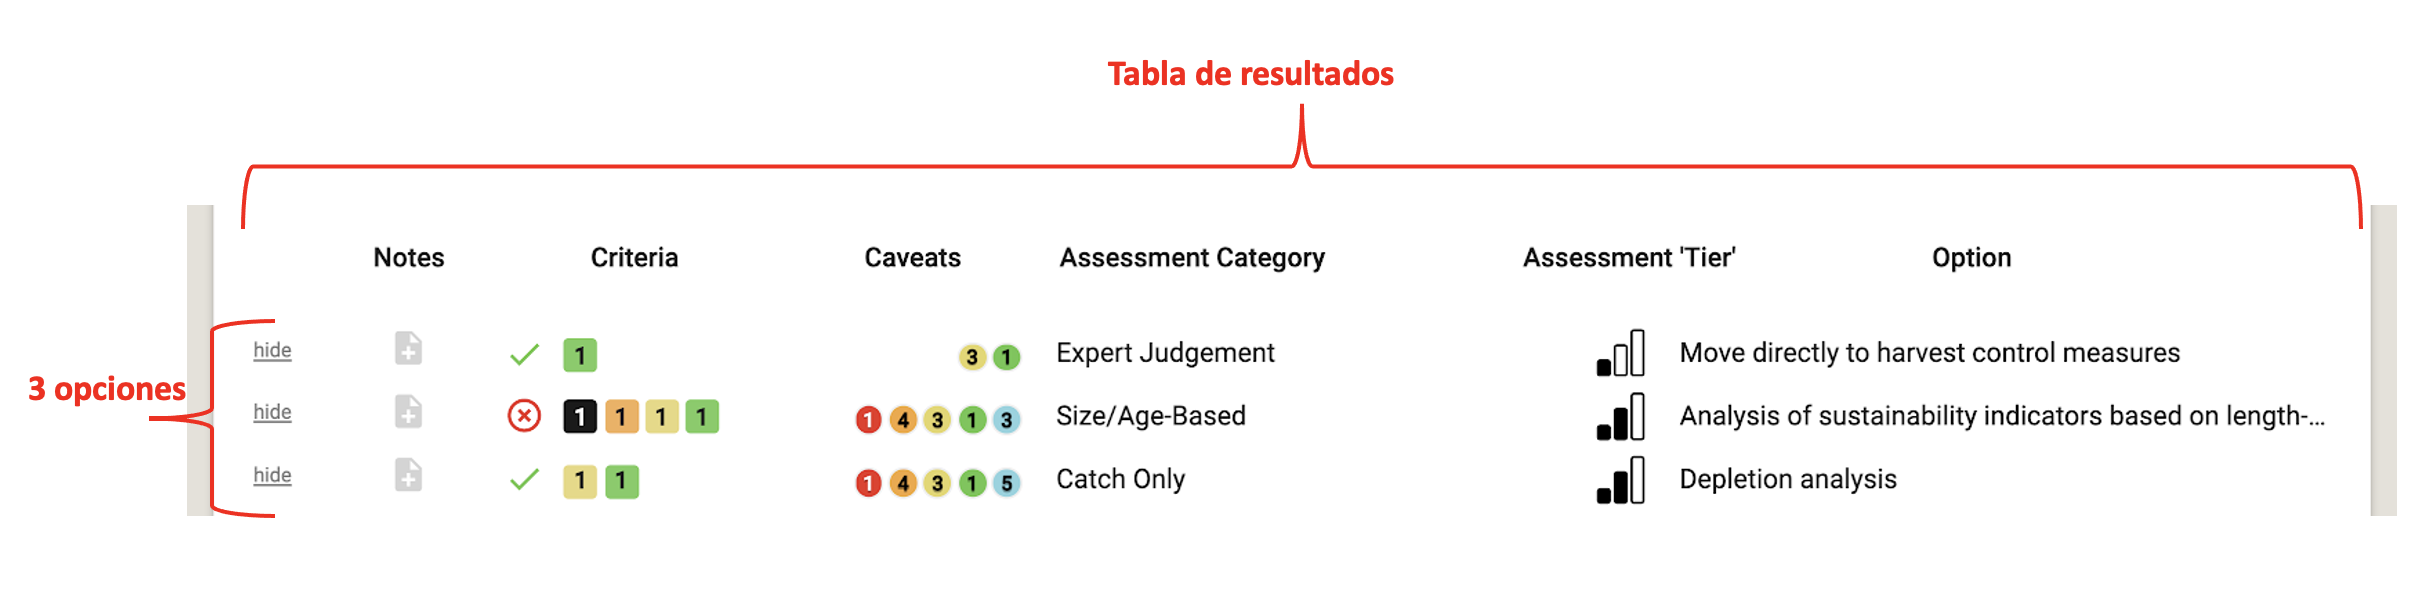
\includegraphics[width=0.95\linewidth]{images/results-rows-es} 

}

\caption{Ejemplo de la tabla de resultados de la herramienta FishPath y 3 opciones (3 filas). Esta es la sección de evaluación.}\label{fig:result-rows}
\end{figure}

\hypertarget{estructura-de-la-tabla}{%
\subsection{Estructura de la tabla}\label{estructura-de-la-tabla}}

\begin{itemize}
\tightlist
\item
  \textbf{Esconder/ Mostrar:} Cualquier opcion para la cual uno o mas de sus mínimos criterios no se cumplieron en la pesquería, son automáticamente ``escondidos'' (se vuelve color gris) por la herramienta FishPath (Figura \ref{fig:hide}). Para cualquier opción, incluyendo las que no cumplen criterios mínimos, los usuarios pueden manualmente hacer click en la opcion ``hide'' -o esconder o en la opción ``unhide''-mostrar. Las opciones escondidas solo se muestran cuando el botón ``Mostrar opciones escondidas'' (o ``Show Hidden Options'') está activada.
\end{itemize}

\begin{figure}

{\centering 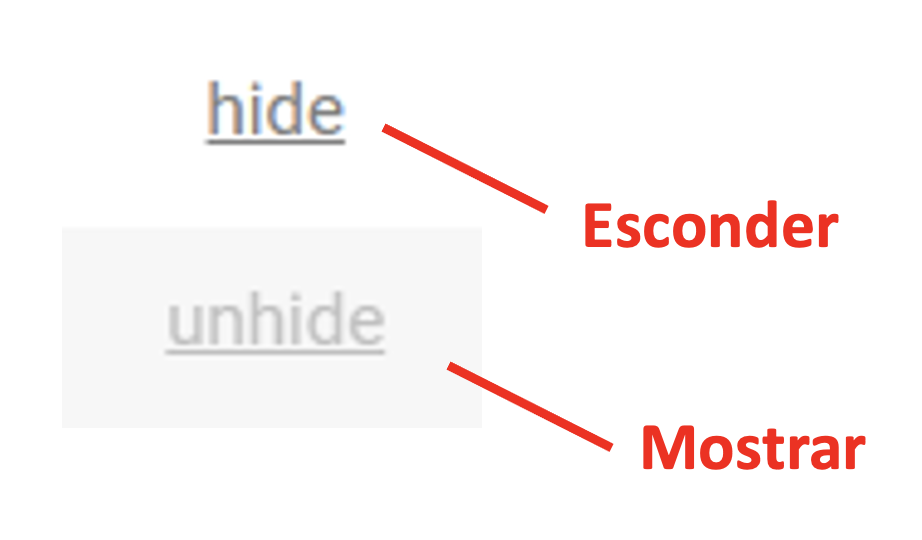
\includegraphics[width=0.1\linewidth]{images/hide-es} 

}

\caption{Habilidad de esconder (“hide”) o mostrar (“unhide”) opciones.}\label{fig:hide}
\end{figure}

\begin{itemize}
\tightlist
\item
  \textbf{Notas:} : Al igual que el cuestionario, las notas pueden ser elaboradas y guardadas (con una conexión estable al internet) para cada opción (Figura \ref{fig:notes}). Las notas pueden incluir detalles específicos de cada pesquería (que no se cubren dentro del cuestionario), por ejemplo, el porqué esa opcion puede ser o no ser una buena elección para la pesquería, o para registrar la opinión del usuario o del grupo sobre esa opcion cuando se consideran las advertencias. Igualmente, las notas pueden ser sobre opciones abiertas o escondidas, para poder usarse como justificación. Las notas serán incluidas en el reporte PDF.
\end{itemize}

\begin{figure}

{\centering 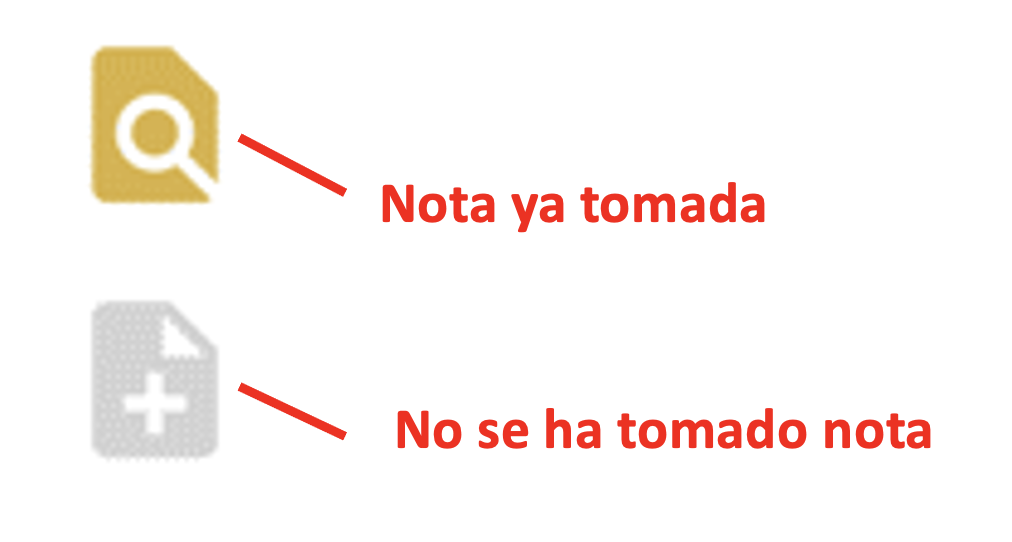
\includegraphics[width=0.15\linewidth]{images/notes-es} 

}

\caption{El ícono superior muestra una opción con una nota ya tomada. Haga clic para ver o editar la nota. El ícono de la parte inferior significa que no se ha tomado nota de la opción. Haga clic para crear una nueva nota.}\label{fig:notes}
\end{figure}

\begin{itemize}
\tightlist
\item
  \textbf{Criterios (Secciones de colecta de datos y evaluación del stock):} La columna de criterios provee información sobre si la pesquería cumple con las condiciones mínimas para poder elegir cierta opción. Si la pesquería cumple dichos criterios, una palomita verde aparecerá. Por otro lado, si la pesquería no cumple con uno o más de los criterios mínimos requeridos para una opción, una cruz roja aparecerá (y la opción es ``escondida'' automáticamente).
\end{itemize}

Para la sección de colecta de datos los criterios son cumplidos o no cumplidos (Figura \ref{fig:dc-criteria}). En una opción eliminada, las cajas color negro indican el numero de criterios mínimos que no fueron cumplidos. Las cajas color verde indican el número de criterios que fueron cumplidos.

\begin{figure}

{\centering 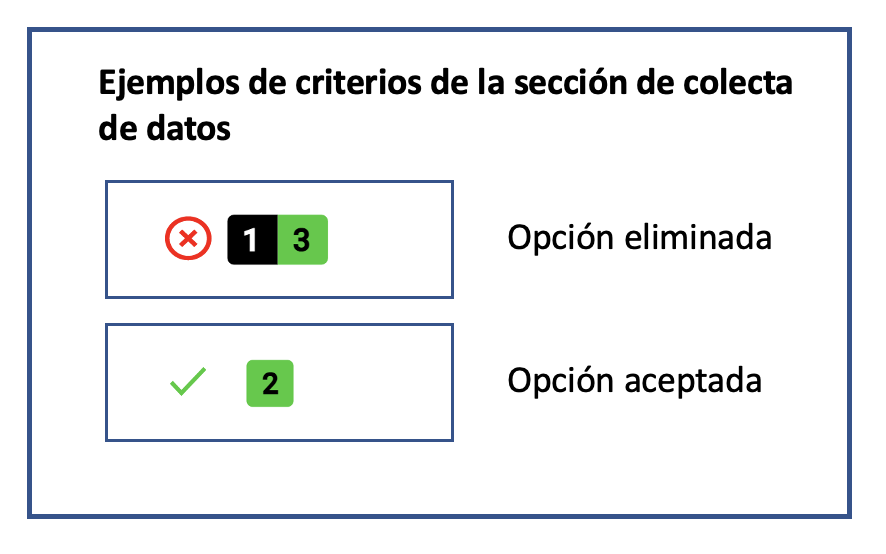
\includegraphics[width=0.35\linewidth]{images/dc-criteria-es} 

}

\caption{Ejemplo de íconos de criterios de colecta de datos. La fila superior muestra una opción que ha sido eliminada, indicada con la cruz roja. Se eliminó debido a que 1 de los 4 criterios no cumplía con el requisito mínimo. La fila inferior muestra una opción que “pasó” o se aceptó, indicada por la palomita verde. La opción cumplió con los requisitos de ambos criterios.}\label{fig:dc-criteria}
\end{figure}

Para la sección de evaluaciones también hay criterios que se cumplen o no cumplen (Figura \ref{fig:a-criteria}). Los criterios que se cumplen tienen colores de semáforo asociados (rojo, anaranjado, amarillo y verde). Los colores representan la calidad de cada tipo de datos y sirven como guía para que los usuarios consideren la incertidumbre asociada a usar dichos datos en los métodos de evaluación. Por ejemplo, se tiene una serie de tiempo de las remociones de la pesquería pero no se cuenta con datos de remoción de una flota importante. La respuesta para esta pregunta reflejará este sesgo. En los resultados, las opciones que requieren series de tiempo de las remociones (de cualquier calidad) desplegarán que este criterio se cumplió, pero se cambiará a color anaranjado para representar que existe alta incertidumbre en los datos de remoción. Esto es un recordatorio de que el usuario necesita considerar la incertidumbre al realizar evaluaciones e interpretar los resultados.

El número de criterios ``No cumplidos'' para cada opción se muestra en la caja negra, mientras que los criterios cumplidos tienen colores que corresponden a cada nivel de incertidumbre. En otras palabras, la caja negra indica el número de criterios mínimos que no fue cumplido, mientras que la suma de los números en las cajas de colores equivalen al número total de critierios cumplidos.

\begin{figure}

{\centering 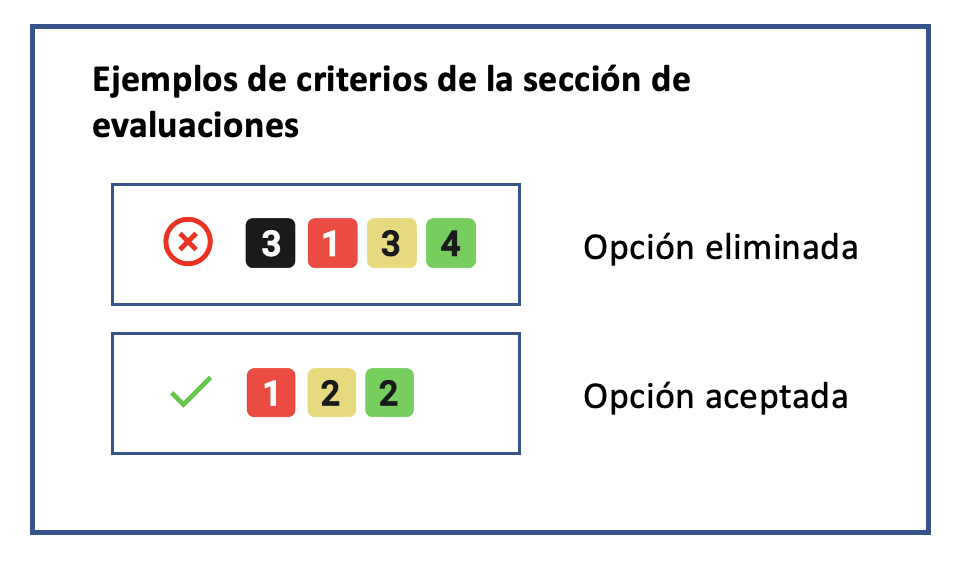
\includegraphics[width=0.35\linewidth]{images/a-criteria-es} 

}

\caption{Ejemplo de los íconos de criterios de evaluación. La fila superior muestra una opción que ha sido eliminada debido a tres criterios que no se cumplieron, cuyo número se puede observar en la caja negra. La fila inferior muestra una opción que cumple con los criterios, representada por una palomita verde. Para ambas filas, cada color de semáforo muestra el número de criterios que cumplen y la severidad de advertencia sobre la incertidumbre.}\label{fig:a-criteria}
\end{figure}

\begin{itemize}
\tightlist
\item
  \textbf{Advertencias:} El formato de la columna de advertencias es el mismo para las tres secciones (Figura \ref{fig:caveats}). Las advertencias se muestran en círculos de colores con números que indican el número total de respuestas del cuestionario que dispararon una advertencia de ese color. Hay tres tipos de advertencia:
\end{itemize}

The format of the caveats column is identical across all three sections (Figure \ref{fig:caveats}). Caveats are shown as colored circles with numbers indicating the total number of questionnaire responses that invoked a caveat of that particular color. There are three types of caveats:

\begin{enumerate}
\def\labelenumi{\arabic{enumi}.}
\tightlist
\item
  \textbf{Advertencias de precaución o cuidado:} Estas son marcadas con círculos rojos, anaranjados y amarillos con la severidad de la advertencia indicada por su color (rojo siendo la mas alta). Estos proveen una guía basada en los atributos de una pesquería. Por ejemplo, si el usuario responde que la especie de interés es susceptible a barotrauma, esto dispararía una advertencia en rojo sobre utilizar límites en la talla de captura como una medida de manejo, debido a la mortalidad por pesca, indicando que los límites de talla no son una medida adecuada.
\item
  \textbf{Atributos positivos:} Un atributo color verde provee razones del porqué una opción puede ser apropiada para la pesquería con base en las respuestas del cuestionario.
\item
  \textbf{Consideraciones estáticas:} Las consideraciones color azul claro son consideraciones estáticas que deben ser tomadas en cuenta, sin importar la pesquería o la respuesta del cuestionario. Una consideración estática es independiente de las circunstancias de una pesquería especifica y por ende siempre están presentes. Estas incluyen supuestos clave para evaluaciones, por ejemplo, la evaluación del stock asume que la selectividad de la pesquería no ha cambiado a través del tiempo o que no puede abordar la incertidumbre.
\end{enumerate}

\begin{figure}

{\centering 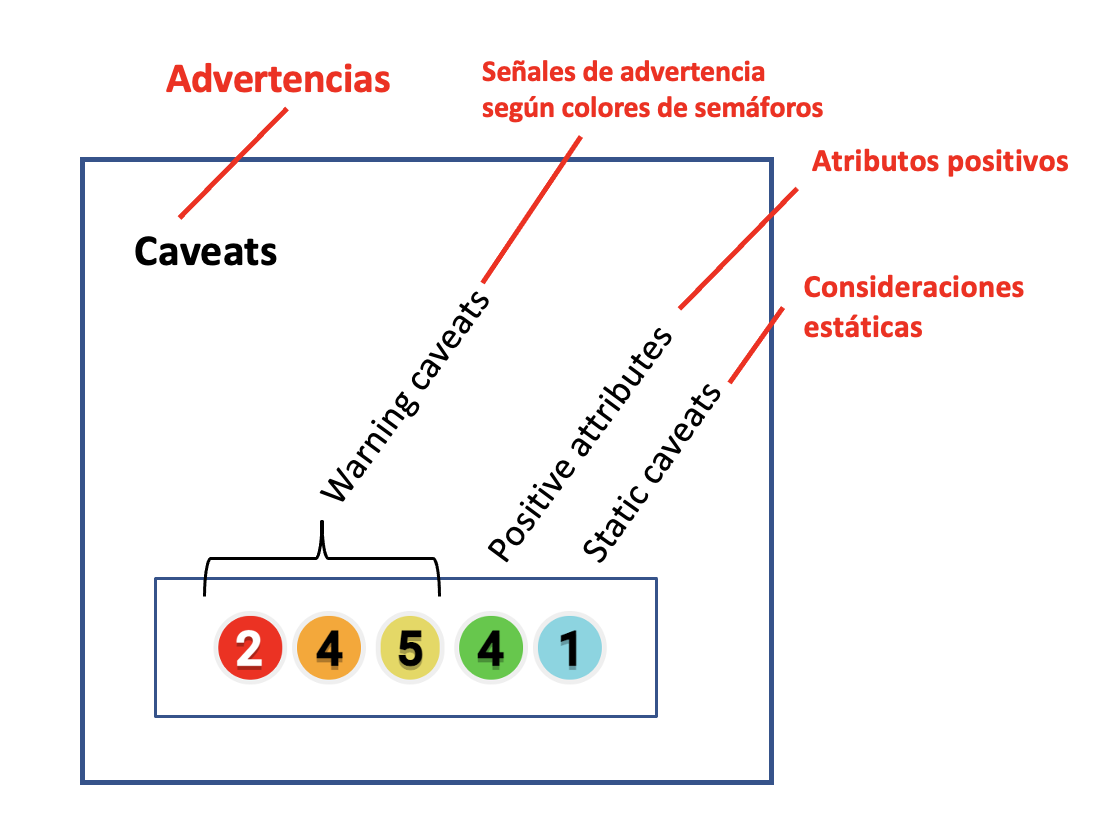
\includegraphics[width=0.35\linewidth]{images/caveats-es} 

}

\caption{Ejemplo del número de advertencias de precaución (colores de semáforo), atributos positivos (verdes) y consideraciones estáticas (azul claro) para una opción.}\label{fig:caveats}
\end{figure}

\begin{itemize}
\tightlist
\item
  \textbf{Categoría:} La columna de categoría permite a los usuarios ver las opciones por categoría. Esta columna es diferente para cada seccion.

  \begin{itemize}
  \item ~
    \hypertarget{Data-Categories}{%
    \paragraph{Categoría de Datos}\label{Data-Categories}}

    En la \textbf{sección de colecta de datos}, la columna ``Data Category'' o categoría de datos muestra las cuatro categorías de datos que pueden ser colectados.

    \begin{enumerate}
    \def\labelenumi{\alph{enumi}.}
    \tightlist
    \item
      \textbf{Entendimiento básico de la pesquería.} Cuando se tiene poco conocimiento de la pesquería, los usuarios podrían empezar colectando información general u operativa de la pesquería para obtener un mejor entendimiento. Donde hay pocos recursos disponibles esta puede ser la única opción de datos/información, aunque se debería aspirar a un esfuerzo que vaya más allá de este paso para hacer el uso más eficiente de la capacidad. La información colectada puede ser dependiente o independiente de la pesquería; puede ayudar a los usuarios a entender más sobre el tamaño y composición de la flota, identificar el tamaño total del área que está siendo pescada, determinar las artes de pesca utilizadas, hacer estimaciones sobre las capturas y esfuerzo, y colectar otra información que ayude a entender la pesquería.
    \item
      \textbf{Análisis de tendencias temporales (series de tiempo).} Los datos colectados para realizar análisis de series de tiempo son usados para monitorear patrones temporales en indicadores de desempeño de la pesquería (captura, esfuerzo, CPUE, y composición de capturas), indicadores ecosistémicos, e indicadores de la biología de las especies. En ausencia de estimadores de biomasa, tendencias temporales de otros indicadores de desempeño pueden ser usados para monitorear la salud de la pesquería a través del tiempo. Los datos para el análisis de tendencias temporales deben ser colectados de manera regular, en intervalos consistentes y comparables (por ejemplo, colectados de las mismas artes de pesca, áreas de pesca similares, etc.).
    \item
      \textbf{Información biológica.} Datos biológicos son colectados al obtener muestras de la población, tomando información biométrica (por ejemplo peso y longitud del organismo), colectando información del sexo y madurez sexual, y/o colectando muestras biológicas para análisis posterior (típicamente relacionadas a la edad, por ejemplo de otolitos, escamas y dientes). Los datos biológicos proveen información clave para el entendimiento de la historia de vida de los organismos, como tasas de crecimiento y reproducción. Estos datos se usan para entender mejor el stock y proveer parámetros que alimentan evaluaciones de stock y modelos que estiman el estado del stock.
    \item
      \textbf{Para informar modelos de evaluación del stock.} El estatus del stock es estimado de manera formal (utilizando modelos de evaluación del stock). Una evaluación del stock provee un indicador (o proxy) del estado del stock, que puede ser comparado con puntos de referencia seleccionados. Los puntos de referencia se usan para indicar si un stock se encuentra en estado deseable o indeseable. Contrario al análisis de de tendencias temporales, los datos colectados aquí son usados para informar una evaluación cuantitativa que resulta en una estimación de la biomasa o mortalidad de pesca, y la categoría se refiere a datos detallados y confiables. Los datos colectados son usados para medir el estado del stock puede incluir series de tiempo robustas, esfuerzo pesquero, CPUE, composiciones de tallas y de peso, densidad dependiente de la pesca o abundancia independiente de la pesca. La mayoría de los métodos de evaluación requieren que cualquier muestreo biológico que se use para informar parámetros biológicos, debería ocurrir antes de, o en conjunto con, esfuerzos de colecta de datos para poder establecer puntos de referencia.
    \end{enumerate}
  \end{itemize}
\end{itemize}

\begin{itemize}
\item ~
  \hypertarget{Assessment-Categories}{%
  \paragraph{Categorías de evaluación}\label{Assessment-Categories}}

  En la \textbf{sección de evaluación}, hay dos tipos de categorías para cada opción. ``\textbf{Categoría de evaluación}'' y ``\textbf{Resultado de la evaluación}''.

  \begin{enumerate}
  \def\labelenumi{\arabic{enumi}.}
  \tightlist
  \item
    \textbf{1. Categoría de la evaluación.} Organiza los métodos de evaluación con base en familias generales de evaluaciones. Esto puede estar relacionado con el tipo de datos requeridos para cada opción (por ejemplo, solamente capturas) o el tipo de evaluación (análisis de riesgo/ vulnerabilidad).

    \begin{enumerate}
    \def\labelenumii{\alph{enumii}.}
    \tightlist
    \item
      \textbf{Indicadores de abundancia.} Abundancia o un proxy de la abundancia es la fuente principal (por ejemplo, captura por unidad de esfuerzo o CPUE).
    \item
      \textbf{Únicamente captura.} Una historia de las capturas (remociones) es la fuente principal. Las opciones pueden usar diversos parámetros de la historia de vida, pero no usan otras series de tiempo o información de capturas basada en talla/edad, tal como de composición de tallas o indicies de abundancia.
    \item
      \textbf{Condición general del stock.} La condición general del stock es determinada por expertos utilizando la información disponible, sin el uso de modelos formales.
    \item
      \textbf{Métodos basados en la historia de vida.} Los parámetros de la historia de vida son utilizados para determinar puntos de referencia que pueden ser usados para comparar con indicadores.
    \item
      \textbf{Áreas Marinas Protegidas o reservas marinas.} Estas pueden comparar lo que hay dentro de una reserva marina y fuera de una reserva marina.
    \item
      \textbf{Indicadores múltiples.} Un marco conceptual que formaliza las medidas de manejo que deben tomarse usando comparaciones entre indicadores múltiples y puntos de referencia.
    \item
      \textbf{Modelos de dinámica poblacional.} Modelos estadísticos integrando dinámica poblacional, por ejemplo, cambios en números y tallas y/o edades en el tiempo.
    \item
      \textbf{Análisis de riesgo/ vulnerabilidad.} Usado para determinar cómo especies o ecosistemas que se encuentran en riesgo reaccionan ante sobrepesca o degradación.
    \item
      \textbf{Basado en edad/tallas.} Estas opciones utilizan la talla o edad de las capturas, tales como la estructura de tallas. Una serie de tiempo de la captura no es necesaria para todas las opciones pero es utilizada por algunas.
    \end{enumerate}
  \item
    \textbf{Resultado de la evaluación.} Los resultados de la evaluación son unidades que la evaluación del stock puede proveer. Hay 5 categorías basadas en los resultados, aunque algunas evaluaciones pueden proveer múltiples resultados .

    \begin{enumerate}
    \def\labelenumii{\alph{enumii}.}
    \tightlist
    \item
      \textbf{Límite de captura.} Los niveles de capturas para aplicarse en medidas de manejo basado en capturas para cumplir objetivos de manejo. Por ejemplo la captura que correspende a un máximo rendimiento sostenible (MSY).
    \item
      \textbf{Tasa de pesca.} La tasa de pesca para ser usada en medidas de manejo basadas en esfuerzo para cumplir objetivos de manejo. Por ejemplo, una tasa de pesca puede ser comparada con un máximo rendimiento sostenible (MSY).
    \item
      \textbf{Estado del stock.} Abundancia relativa del stock.
    \item
      \textbf{Escala del stock.} La abundancia absoluta del stock.
    \item
      \textbf{Otras métricas de reglas de control.} Cualquier indicador que no sea de los cuatro enumerados anteriormente, ejemplo: cambio en la composición de especies en las capturas.
    \end{enumerate}
  \end{enumerate}
\item ~
  \hypertarget{Management-Measure-Categories}{%
  \paragraph{Categorías de medidas de manejo}\label{Management-Measure-Categories}}

  En la \textbf{sección de medidas de manejo} esta columna se llama ``Categoría'' y muestra las categorías de medidas de manejo. Hay 8 categorías de medidas de manejo.

  \begin{enumerate}
  \def\labelenumi{\alph{enumi}.}
  \tightlist
  \item
    \textbf{Limites de captura.} Los límites de captura buscan manejar de manera directa la mortalidad por pesca de las especies que son capturadas, al establecer un máximo del número de individuos, o el peso a ser capturado en la pesquería en un periodo de tiempo dado y/o en áreas específicas.
  \item
    \textbf{Límites de esfuerzo.} Los límites de esfuerzo buscan manejar la mortalidad por pesca ajustando la actividad de pesca de las flotas, para alinear con una tasa de explotación pesquera que logre objetivos de manejo. Es una forma de controlar la entrada, los límites de esfuerzo pesquero impactan todas las especies sujetas a la pesca, y no solamente especies objetivo. Los límites de esfuerzo pueden ser útiles al manejar pesquerías multiespecíficas (donde el control de capturas específico a una especie puede ser difícil de implementar) en pesquerías donde el arte de pesca o esfuerzo son raramente controlados o en pesquerías donde la captura reportada no es fiable.
  \item
    \textbf{Manejo de las artes de pesca.} Las artes de pesca especifican el tipo y diseño del equipo permitido en en una pesquería para controlar la eficiencia y capacidad de cosecha de los pescadores.
  \item
    \textbf{Manejo temporal.} El manejo temporal regula las capturas, limitando el número de días u horas que la pesquería está abierta. El objetivo es controlar la mortalidad por pesca. Esto incluye reglas establecidas o reglas que son modificadas de acuerdo a los resultados obtenidos de una evaluación.
  \item
    \textbf{Manejo espacial.} El manejo espacial involucra aplicar medidas de manejo que son espacialmente explícitas, osea específicas a una o varias áreas de pesca dentro de la distribución de la pesquería. El manejo espacial incluye el uso temporal, rotatorio o permanente de reservas, cierres espaciales o áreas marinas protegidas. También puede incluir reglas que limitan la captura individual o el esfuerzo pesquero en una sola área, requiriendo que los pescadores se muevan a otra área si los límites se excedieron. Reglas de control de cosecha espaciales pueden pueden proteger ciertas áreas de impactos directos e indirectos de la pesca, lo cual a su vez afecta el ecosistema entero dentro de las áreas restringidas. Las restricciones espaciales pueden ser permanentes o pueden modificarse.
  \item
    \textbf{Límites de talla.} Los límites de talla especifican la talla/ tamaño en el cual las especies pueden ser legalmente capturadas. En el contexto de una estrategia de cosecha los límites de talla generalmente buscan proteger ciertas etapas de vida del organismo (por ejemplo juveniles) con el fin de incrementar la productividad o mantener sostenibilidad de la pesquería.
  \item
    \textbf{Regulaciones relacionadas al género del organismo.} Regulaciones de reproducción pueden ser implementadas en especies donde machos y hembras maduran a distintas tallas/tamaños, ya sea debido a diferencias en su tasa de crecimiento o madurez sexual - relacionado al género. Las regulaciones pueden ser aplicadas separadamente para cada género para promover que los individuos alcancen la madurez sexual antes de ser cosechados.
  \item
    \textbf{Otro} Esta categoría de manejo incluye otras opciones que no son capturadas en las categorías mencionadas anteriormente.
  \end{enumerate}
\end{itemize}

\begin{itemize}
\item ~
  \hypertarget{nivel-de-evaluaciuxf3n-uxfanicamente-para-la-evaluaciuxf3n}{%
  \paragraph{``Nivel de evaluación'' (Únicamente para la evaluación)}\label{nivel-de-evaluaciuxf3n-uxfanicamente-para-la-evaluaciuxf3n}}
\end{itemize}

La disponibilidad de métodos analíticos incrementa cuando los datos e información biológica incrementan, por esta razón entre más información se tenga más métodos se hacen disponibles. Algunos de los métodos más simples podrían ya no ser candidatos fuertes para la aplicación cuando se compara con métodos que requieren de más datos. La categoría del ``nivel de evaluación'' ayuda a determinar de manera general los datos requeridos y el nivel de complejidad de cada modelo. Esto es útil cuando se busca priorizar los métodos de evaluación ya que permite al usuario identificar que método es más apropiado para sus datos, en vez de tratar de hacer todos los métodos posibles. Una recomendación general es considerar priorizar los métodos con un nivel de evaluación más alto, cuando se busca elegir métodos para implementar, aunque esto no excluye los métodos de nivel de evaluación más bajos. Se recomienda que el usuario considere los beneficios y costos entre las altas capacidades técnicas y la incertidumbre de los datos asociados a métodos con nivel de evaluación más alto, versus la baja demanda de datos y capacidad técnica de los métodos con nivel de evaluación baja, pero su limitada robustez. Para poder hacer énfasis en métodos más rigurosos, los métodos de ``priorización del stock'' y ``extremadamente deficientes de datos'' son automáticamente escondidos cuando hay otras opciones disponibles, de nivel medio a alto.

Hay 5 niveles de evaluación:

\begin{enumerate}
\def\labelenumi{\alph{enumi}.}
\item
  \textbf{Pre-assessment o pre evaluación -- Priorización del stock (SP):} Métodos en este nivel identifican especies o grupos de especies que pueden ser clasificados como en riesgo y ayuda a priorizar los stocks que deben ser considerados para manejo.
\item
  \textbf{Pre-assessment o pre evaluación -- Puntos de referencia basados en la historia de vida (RP):} Estos métodos proveen puntos de referencia que pueden ser utilizados en otros métodos de evaluación.
\item
  \textbf{Extremely data-poor o extremadamente deficientes en datos (Una barra):} Métodos que brindan orientacion para el manejo con un mínimo de datos disponibles. Si hay niveles medios y altos disponibles entonces el usuario debería enfocarse en estos.
\item
  \textbf{Medio (dos barras):} Métodos que requieren una cantidad moderada de datos, usualmente colectados a lo largo de una serie de tiempo. Estos incluyen métodos basados en tallas, en capturas o marcos conceptuales con indicadores múltiples.
\item
  \textbf{Alto (tres barras):} Métodos que necesitan la cantidad más intensiva de datos y modelos computacionales, por ejemplo, modelos de dinámica poblacional.
\end{enumerate}

\begin{itemize}
\tightlist
\item
  \textbf{Opción:} Este es el nombre de la opción.
\end{itemize}

\hypertarget{detalles-completos-de-las-opciones}{%
\subsection{Detalles completos de las opciones}\label{detalles-completos-de-las-opciones}}

Cada fila dentro de la tabla de resultados muestra el nombre de la opción con un resumen de los resultados para cada opción. Cuando los usuarios hacen click en alguna opción, una ventana emergente aparece, la cual provee detalles completos de la opción misma, en conjunto con los detalles de cada criterio y advertencia.

Primeramente, se provee una descripción de la opción, en conjunto con las referencias relevantes y la información de contacto (si se encuentra disponible o si es apropiado). Para las opciones de colecta de datos, los tipos de datos que pueden ser colectados según la opción son resumidos. Para la seccion de evaluación del stock, cuando se encuentre disponible, links para paquetes de evaluación de stocks son provistos.

Posteriormente, los criterios y advertencias que surgieron son resumidos como se muestra en la Figura \ref{fig:opt-desc}

\begin{itemize}
\tightlist
\item
  Criterios no cumplidos,
\item
  Criterios cumplidos,
\item
  Advertencias de precaución,
\item
  Atributos positivos y
\item
  Consideraciones estáticas
\end{itemize}

A la par de cada uno, se encuentran menús desplegables individuales donde el usuario puede encontrar detalles específicos de cada criterio y advertencia, en conjunto con la pregunta y respuesta que disparó estos criterios o advertencias.

\begin{figure}

{\centering 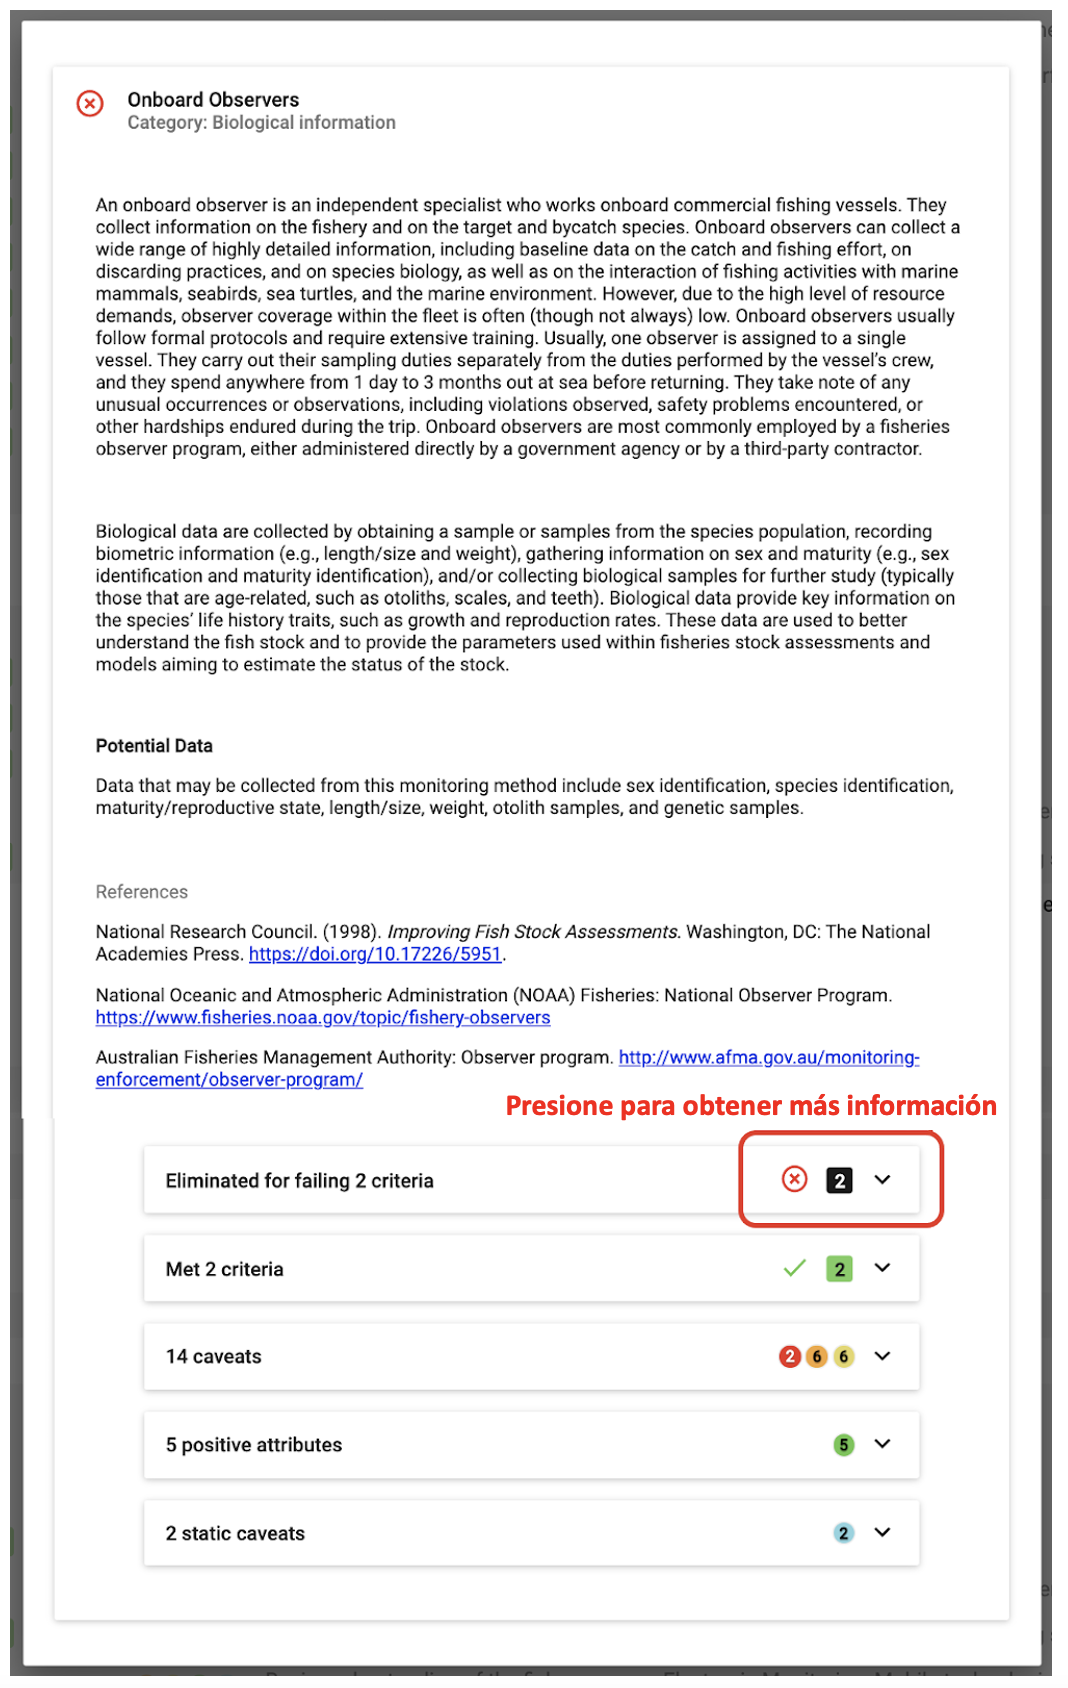
\includegraphics[width=0.5\linewidth]{images/option-description-es} 

}

\caption{Example of pop-up box that appears when clicking on each option. The user may click to expand each drop down menu for detail on each criteria or caveat (red label “Click to expand”).}\label{fig:opt-desc}
\end{figure}

\textbf{Menú desplegable para los criterios (Figures \ref{fig:crit-drop-down}-\ref{fig:assessment-crit-drop-down})}: Cada menú desplegable de los criterios muestra las preguntas más relevantes con las respuestas provistas por el usuario (marcados en negro) relativo al nivel mínimo requerido para esa opción (en donde el color verde inicia a la izquierda - Figura \ref{fig:crit-drop-down}).

Para la sección de evaluación, cuando los criterios mínimos se cumplen, colores de semáforo son asignados para indicar la incertidumbre relativa y subsecuentemente, la precaución que se debería tomar (Figura \ref{fig:assessment-crit-drop-down}).

\begin{figure}

{\centering 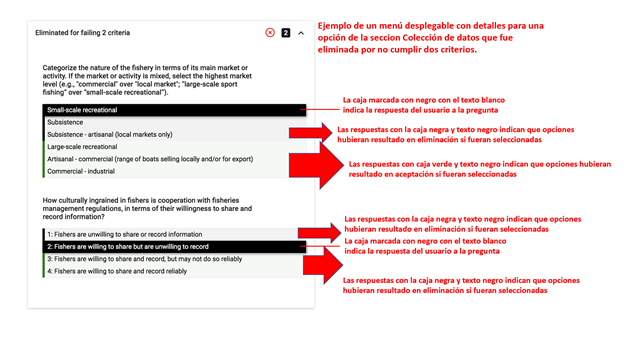
\includegraphics[width=0.75\linewidth]{images/crit-drop-down-es} 

}

\caption{. Ejemplo de un menú desplegable con los detalles para una opción dentro de la seccion colecta de datos al no cumplir con dos criterios, la explicación de cada parte se encuentra en la figura.}\label{fig:crit-drop-down}
\end{figure}

\begin{figure}

{\centering 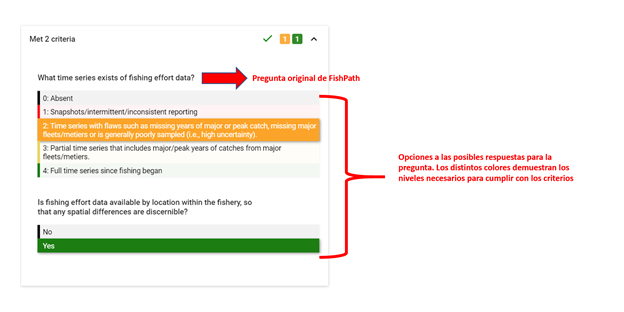
\includegraphics[width=0.75\linewidth]{images/assessment-crit-drop-down-es} 

}

\caption{Ejemplo de un menú desplegable con detalles para una opción en la sección de evaluación que cumplió los criterios, pero indica al usuario precaución relacionada a la incertidumbre en los datos de remoción. El rojo indica alta incertidumbre en los datos. El verde indica baja incertidumbre. La caja de color con texto blanco indica la respuesta del usuario.}\label{fig:assessment-crit-drop-down}
\end{figure}

\textbf{Cajas desplegables para las advertencias (Figuras \ref{fig:cav-drop-down}-\ref{fig:static-cav-drop-down})}: Cada advertencia tiene su caja desplegable que muestra la pregunta de FishPath con la respuesta del usuario en gris, seguido de la descripción de la advertencia relacionada al uso de la opción en esa pesquería en el contexto particular de esa respuesta. El color de cada caja refleja el color de la advertencia (ver descripciones de advertencias): advertencias de precaución en color amarillo, anaranjado o rojo; atributos positivos en verde; y los consideraciones estáticas en color azul claro.

\begin{figure}

{\centering 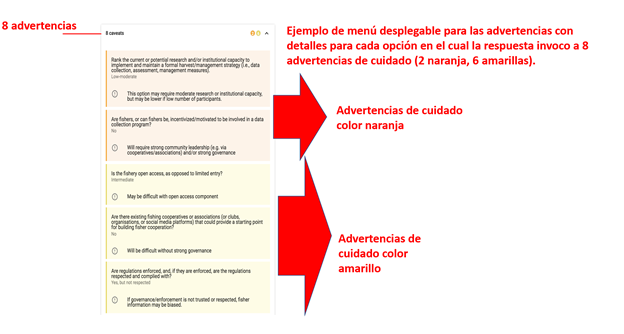
\includegraphics[width=0.75\linewidth]{images/cav-drop-down-es} 

}

\caption{Ejemplo de menú desplegable para las advertencias con detalles para una opción en la cual las respuestas en el cuestionario dispararon 8 advertencias de precaución (2 anaranjadas, 6 amarillas).}\label{fig:cav-drop-down}
\end{figure}

\begin{figure}

{\centering 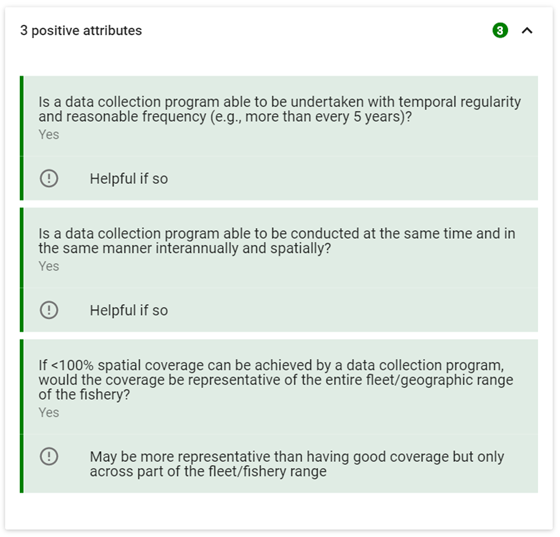
\includegraphics[width=0.75\linewidth]{images/pos-attr-drop-down-es} 

}

\caption{Ejemplo de un menú desplegable de los posibles atributos positivos para una opción para cual el cuestionario presenta 3 atributos positivos (se encuentran en la esquina superior derecha del menú desplegable).}\label{fig:pos-attr-drop-down}
\end{figure}

\begin{figure}

{\centering 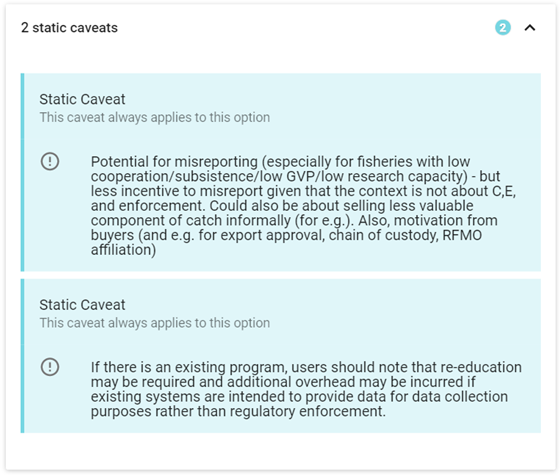
\includegraphics[width=0.75\linewidth]{images/static-cav-drop-down-es} 

}

\caption{Ejemplo de una opción con 2 consideraciones estáticas (se encuentran en la esquina superior derecho del menú desplegable). Cada caja de las consideraciones estáticas presenta una nota en gris que dice “Esta consideración siempre se aplica a esta opción”, y una breve explicación de la misma.}\label{fig:static-cav-drop-down}
\end{figure}

\hypertarget{Filters-Sorting}{%
\section{Mostrar opciones escondidas y ordenar opciones}\label{Filters-Sorting}}

El botón ``Mostrar opciones escondidas'' (Figura \ref{fig:show-hidden-sort}) permite al usuario mostrar o no mostrar las opciones que han sido ``escondidas'' (coloreadas en gris). Cuando es activado, las opciones ``escondidas'' aparecerán en gris.

\begin{figure}

{\centering 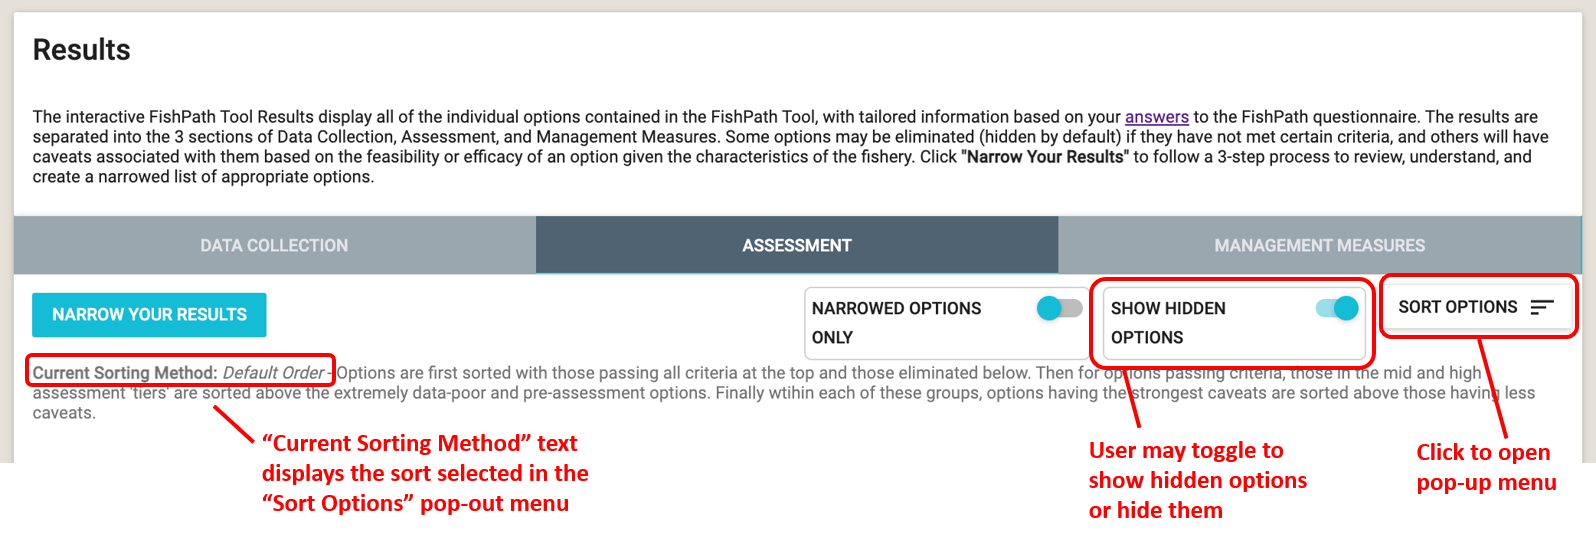
\includegraphics[width=0.75\linewidth]{images/show-hidden-options-and-sort} 

}

\caption{Página de resultados con el botón de “Mostrar opciones escondidas” y “Ordenar opciones” dentro de un circulo rojo.}\label{fig:show-hidden-sort}
\end{figure}

La funcionalidad de ``Ordenar opciones'' permite al usuario odenar y ver las opciones de distintas maneras. Esto no afecta los resultados o elimina resultados, simplemente es una manera de poder organizar y visualizar sus resultados. El orden seleccionado se muestra en la parte superior de la tabla de resultados en ``Orden actual'' o ``Current Sorting Method'' (Figura \ref{fig:show-hidden-sort}).

Después de presionar ``Ordenar opciones'', una caja aparecerá (Figura \ref{fig:filter-and-sorting}) con la habilidad de ordenar las opciones de acuerdo a:

\begin{itemize}
\tightlist
\item
  Únicamente para la sección de evaluación, hay una opción adicional para ordenar las opciones: ``Categoría de evaluación'' (o ``Assessment Category'') o ``Resultados de la evaluación'' (o ``Assessment Output'').
\item
  \textbf{Orden predeterminado:} El orden predeterminado enlista todas las opciones que no cumplieron con el criterio mínimo en la parte inferior (automáticamente sombreado de color gris como opciones escondidas), con las opciones para las cuales el mayor número de advertencias fueron invocadas en la parte superior.
\item
  \textbf{Orden personalizado:} Este mantiene el orden actual pero permite al usuario retornar a la tabla de resultados y ``arrastrar y soltar'' opciones en un orden preferido.
\item
  \textbf{Ordenar por el ``nivel de evaluación'' (únicamente para la sección de evaluación):} Ordena las opciones de acuerdo a su complejidad y requerimiento o demanda de datos
\item
  \textbf{Ordenar por medio del nombre de la opción:} Ordena las opciones alfabéticamente por el nombre de la opción.
\item
  \textbf{Ordenar por categoría:} Ordena las opciones alfabéticamente por el nombre de cada categoría. Para la seccion de evaluación, los usuarios primeramente deben seleccionar la categoría que quieren visualizar y ordenar.
\end{itemize}

Al presionar ``ordenar opciones'', automáticamente se ordenarán todas las opciones en la pantalla. Después de hacer selecciones en la ventada de ordenar, los usuarios pueden hacer clic en los resultados fuera de la ventana emergente para retornar a los resultados.

\begin{figure}

{\centering 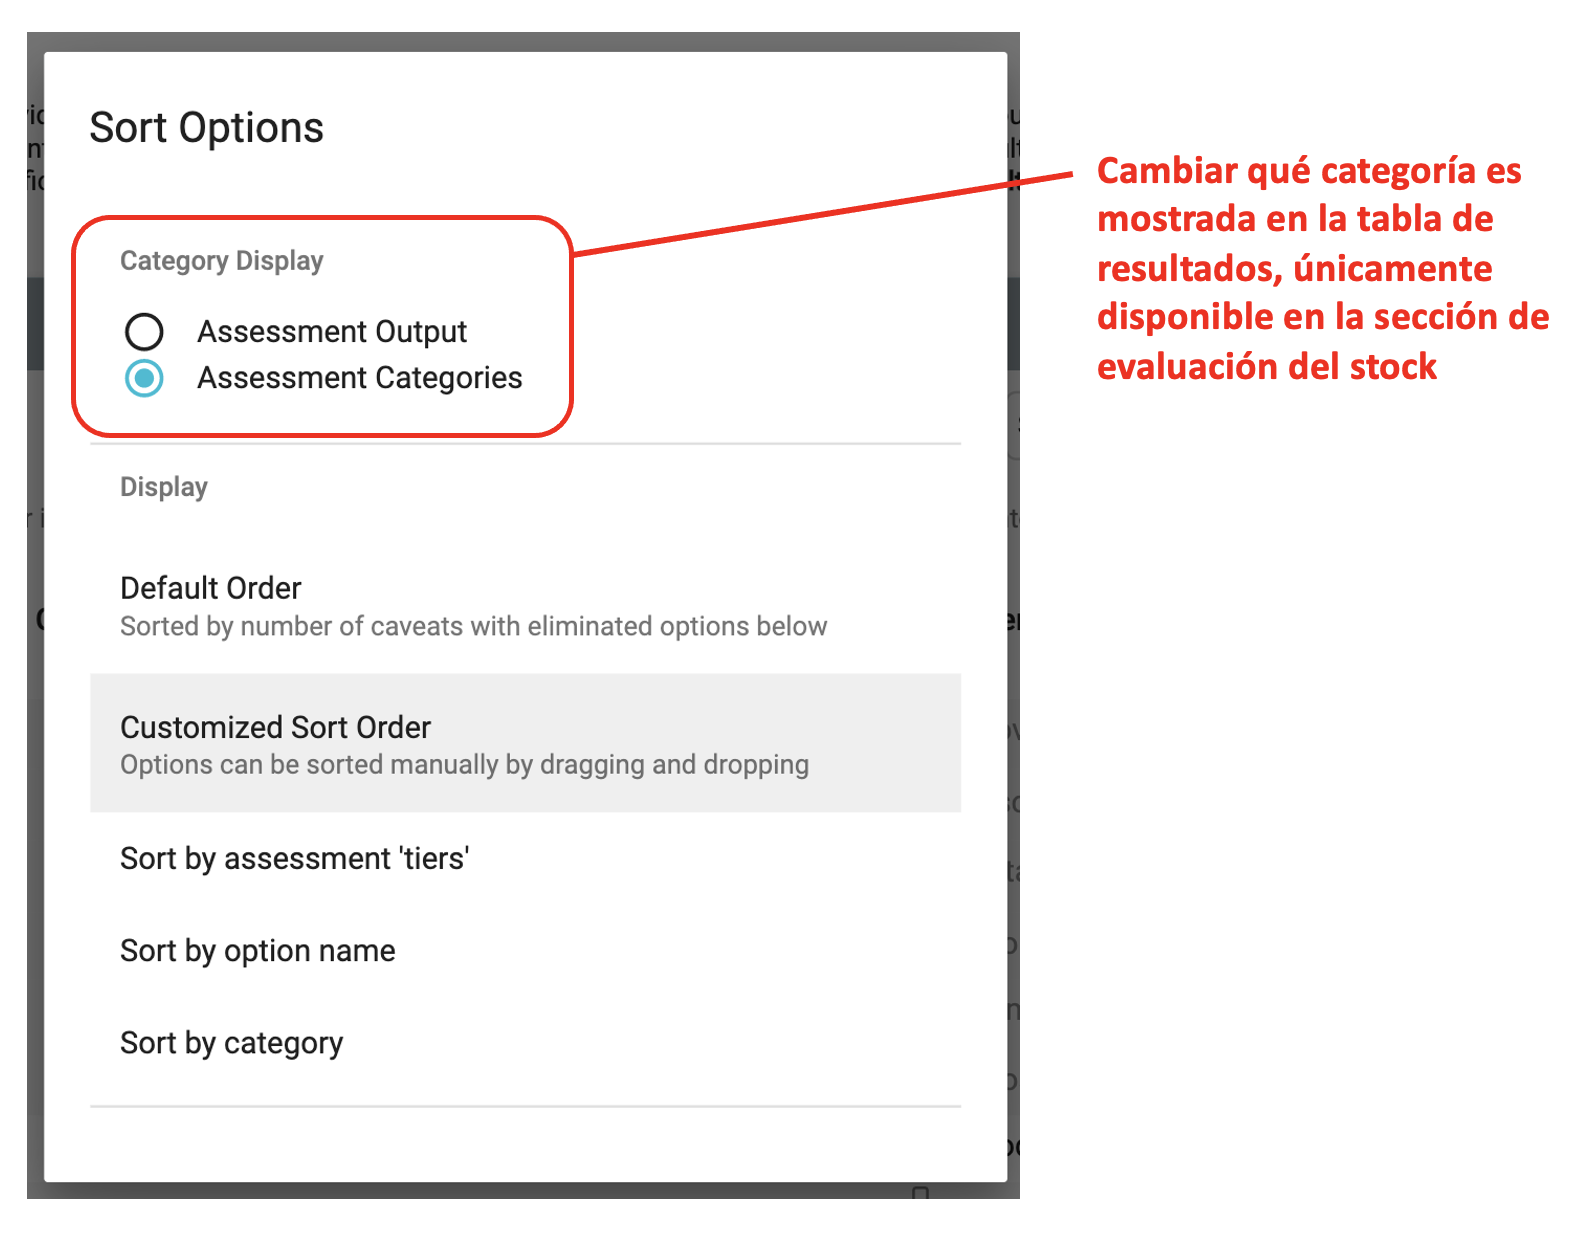
\includegraphics[width=0.5\linewidth]{images/filter-and-sorting-assessment-es} 

}

\caption{Ventana emergente para ordenar las opciones.}\label{fig:filter-and-sorting}
\end{figure}

\hypertarget{Bookmark-Influential}{%
\section{Preguntas marcadas y respuestas influyentes}\label{Bookmark-Influential}}

Si el usuario se desplaza a la parte interior de la pantalla de resultados (debajo de la tabla de resultados), se provee una lista resumida de las preguntas que fueron marcadas por el usuario, en conjunto con una lista de las ``respuestas influyentes'' y un link de ``ver todas sus respuestas''.

\hypertarget{preguntas-marcadas}{%
\subsection{Preguntas marcadas}\label{preguntas-marcadas}}

Todas las preguntas que fueron ``marcadas'' durante el cuestionario serán enlistadas acá (Figura \ref{fig:flagged-questions}). Los usuarios pueden seleccionar cada pregunta para obtener una lista detallada de las advertencias generadas o los criterios que no fueron cumplidos basados en su respuesta. Los usuarios también pueden seleccionar cada pregunta para cambiar la respuesta, añadir notas o eliminar la marca. Es altamente recomendable revisar estas preguntas y las advertencias para que los usuarios puedan actualizar sus respuestas o proveer notas más detalladas sobre su respuesta, al ver cómo sus respuestas impactan sus resultados.

\begin{figure}

{\centering 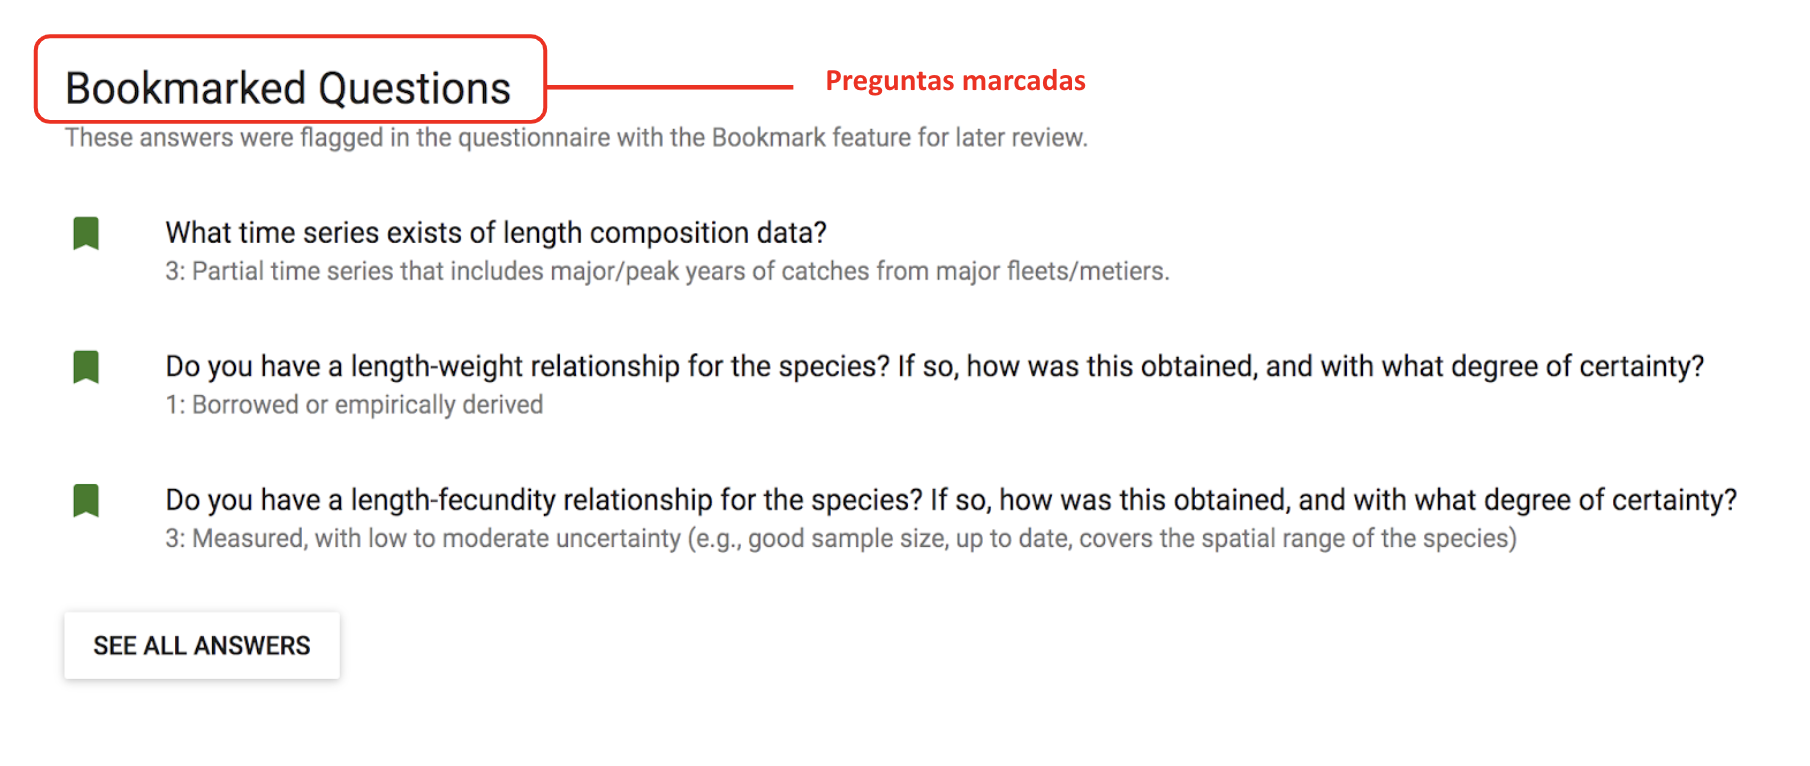
\includegraphics[width=0.95\linewidth]{images/flagged-questions-es} 

}

\caption{Lista de preguntas marcadas.}\label{fig:flagged-questions}
\end{figure}

\hypertarget{preguntas-influyentes}{%
\subsection{Preguntas influyentes}\label{preguntas-influyentes}}

La lista de ``Respuestas influyentes'' es un resumen de las preguntas y respuestas de los usuarios que resultaron en el mayor número de criterios eliminatorios y el mayor número de precauciones fuertes (Figura \ref{fig:influential-answers}). Los criterios y precuaciones disparados por estas preguntas se muestran con íconos a la izquierda de la pregunta por número e intensidad del color.

Se recomienda revisar esta lista antes de entrar al proceso de reducir los resultados (descrito a continuación), para entender mejor algunos de los retos clave que esa pesquería enfrenta. Los usuarios pueden seleccionar cualquier pregunta en esta lista para cambiar una respuesta, añadir notas a la pregunta y ver una lista de todas las opciones impactadas y sus advertencias asociadas (Figura \ref{fig:influential-answers-expanded}).

\begin{figure}

{\centering 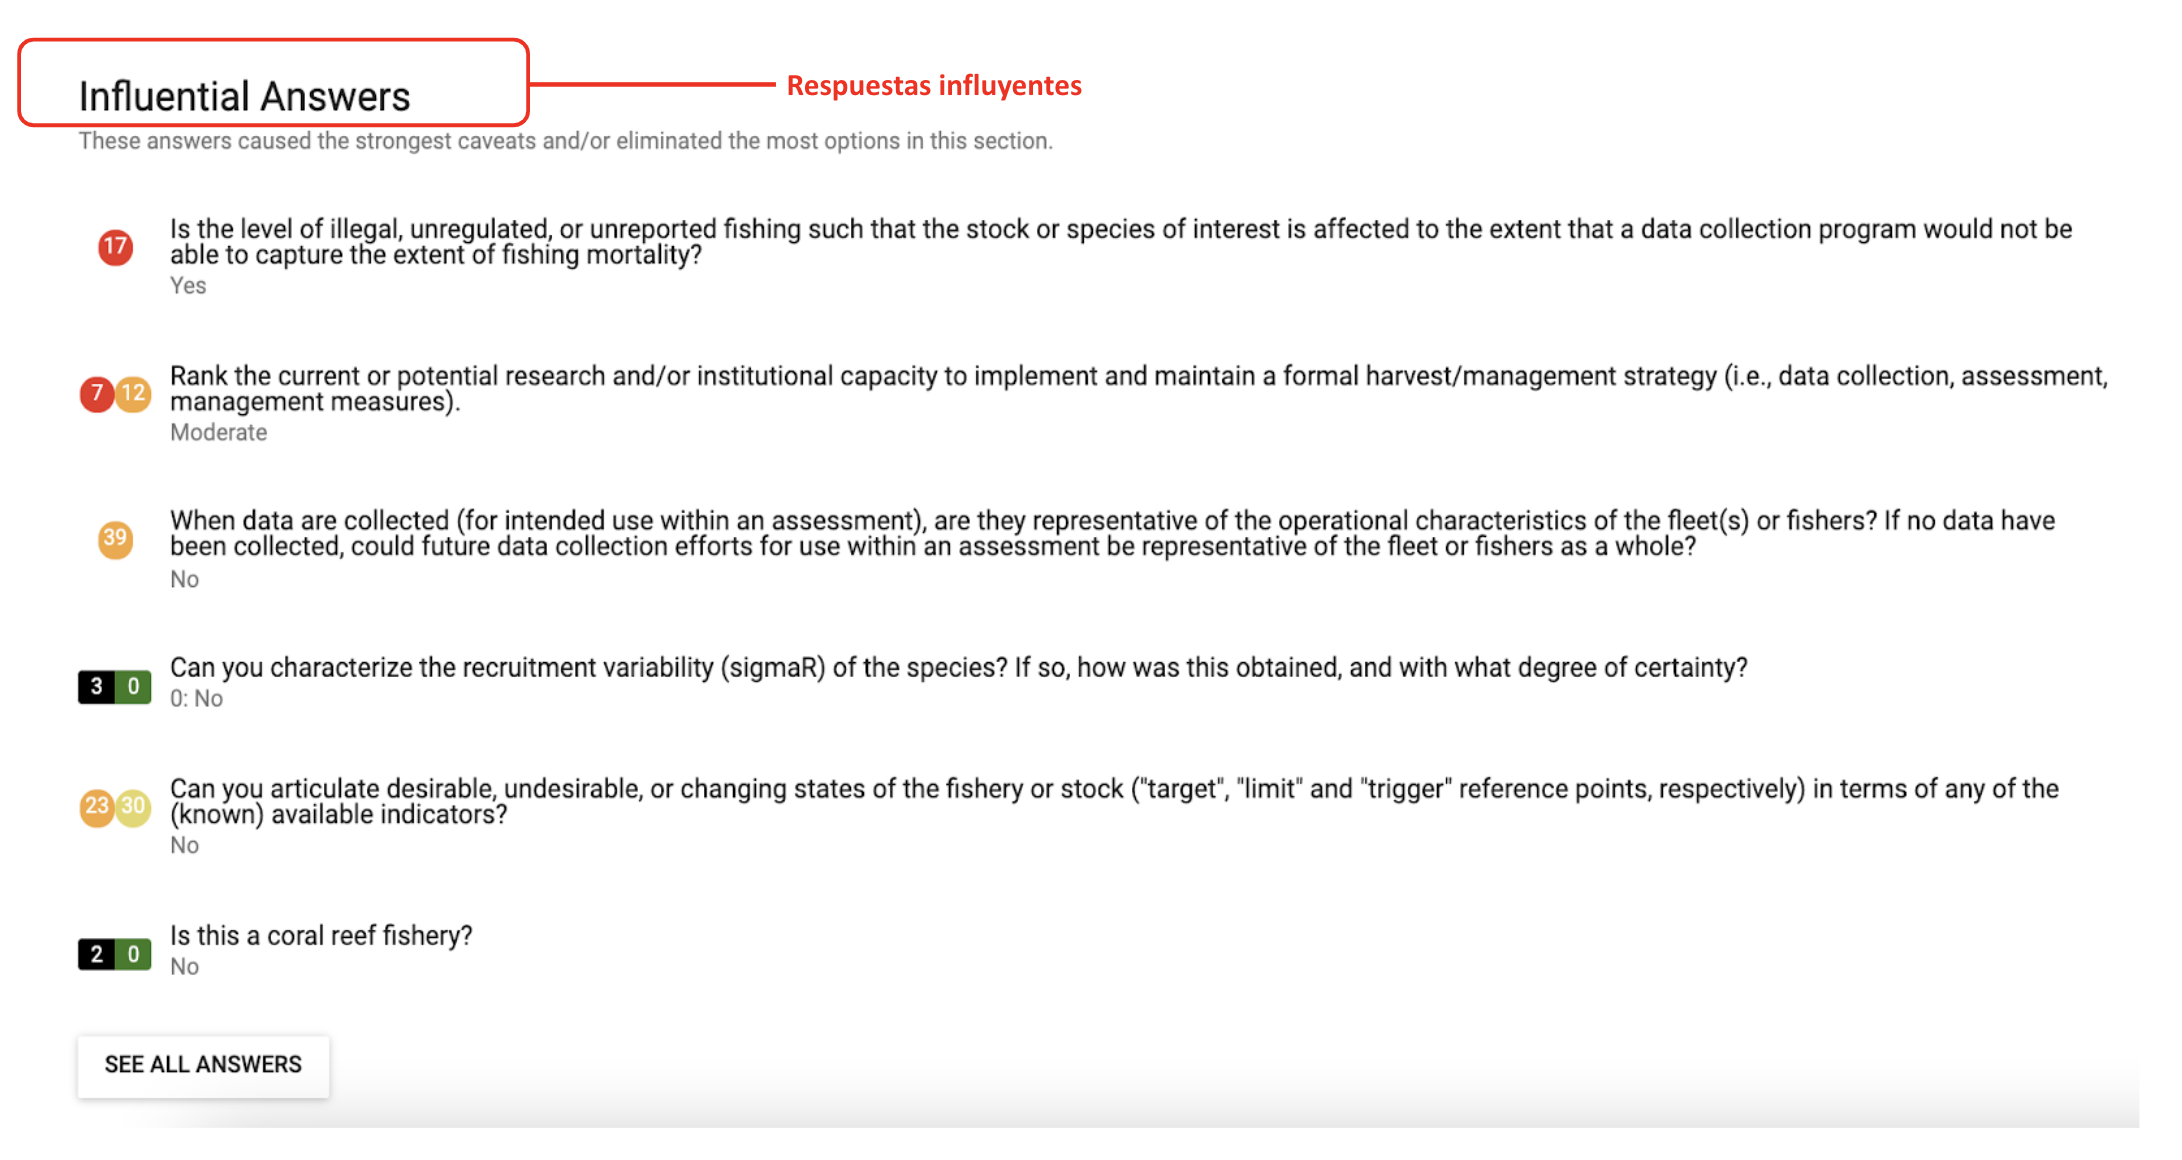
\includegraphics[width=0.95\linewidth]{images/influential-answers-es} 

}

\caption{Lista de respuestas influyentes.}\label{fig:influential-answers}
\end{figure}

\begin{figure}

{\centering 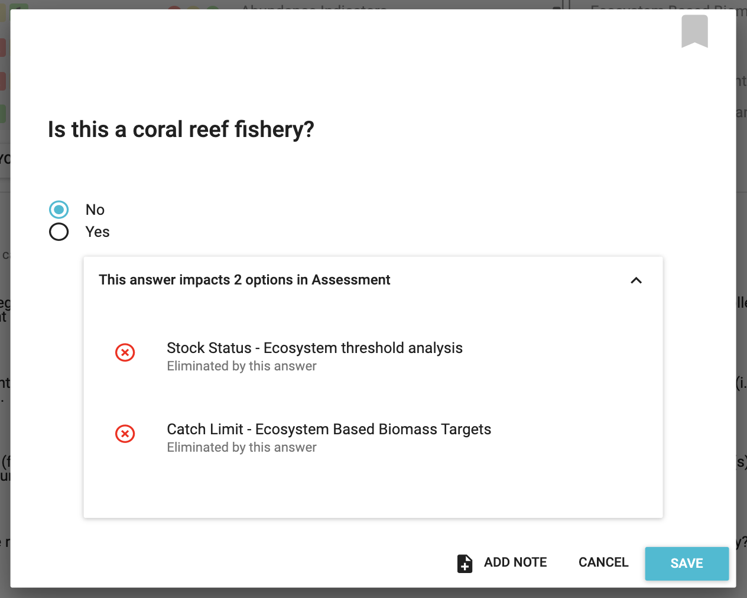
\includegraphics[width=0.75\linewidth]{images/influential-answers-expanded} 

}

\caption{Al hacer click en una pregunta en la lista de “Respuestas influyentes”, una ventana emergente aparece, permitiendo al usuario ver las op ciones impactadas.}\label{fig:influential-answers-expanded}
\end{figure}

\hypertarget{ver-todas-las-respuestas}{%
\subsection{Ver todas las respuestas}\label{ver-todas-las-respuestas}}

Hay 2 maneras para que el usuario pueda ver todas sus respuestas del cuestionario. Primero, en la parte de arriba de la página, los usuarios pueden presionar el link llamado ``answers'' (o respuestas) en el párrafo debajo del encabezado ``results''. Segundo, en la parte de abajo de la página hay un botón llamado ``See all answers'' o ``Ver todas las respuestas''. Después de hacer click en cualquiera de estas opciones, el usuario es dirigido a la página de respuestas que incluye una lista completa de todas las secciones con sus detalles correspondientes. Este es un buen recurso para usuarios que quieran revisar sus respuestas y notas asociadas a una pesquería. Las respuestas pueden ser modificadas y se pueden agregar notas las cuales se actualizan después de guardar los cambios.

\begin{figure}
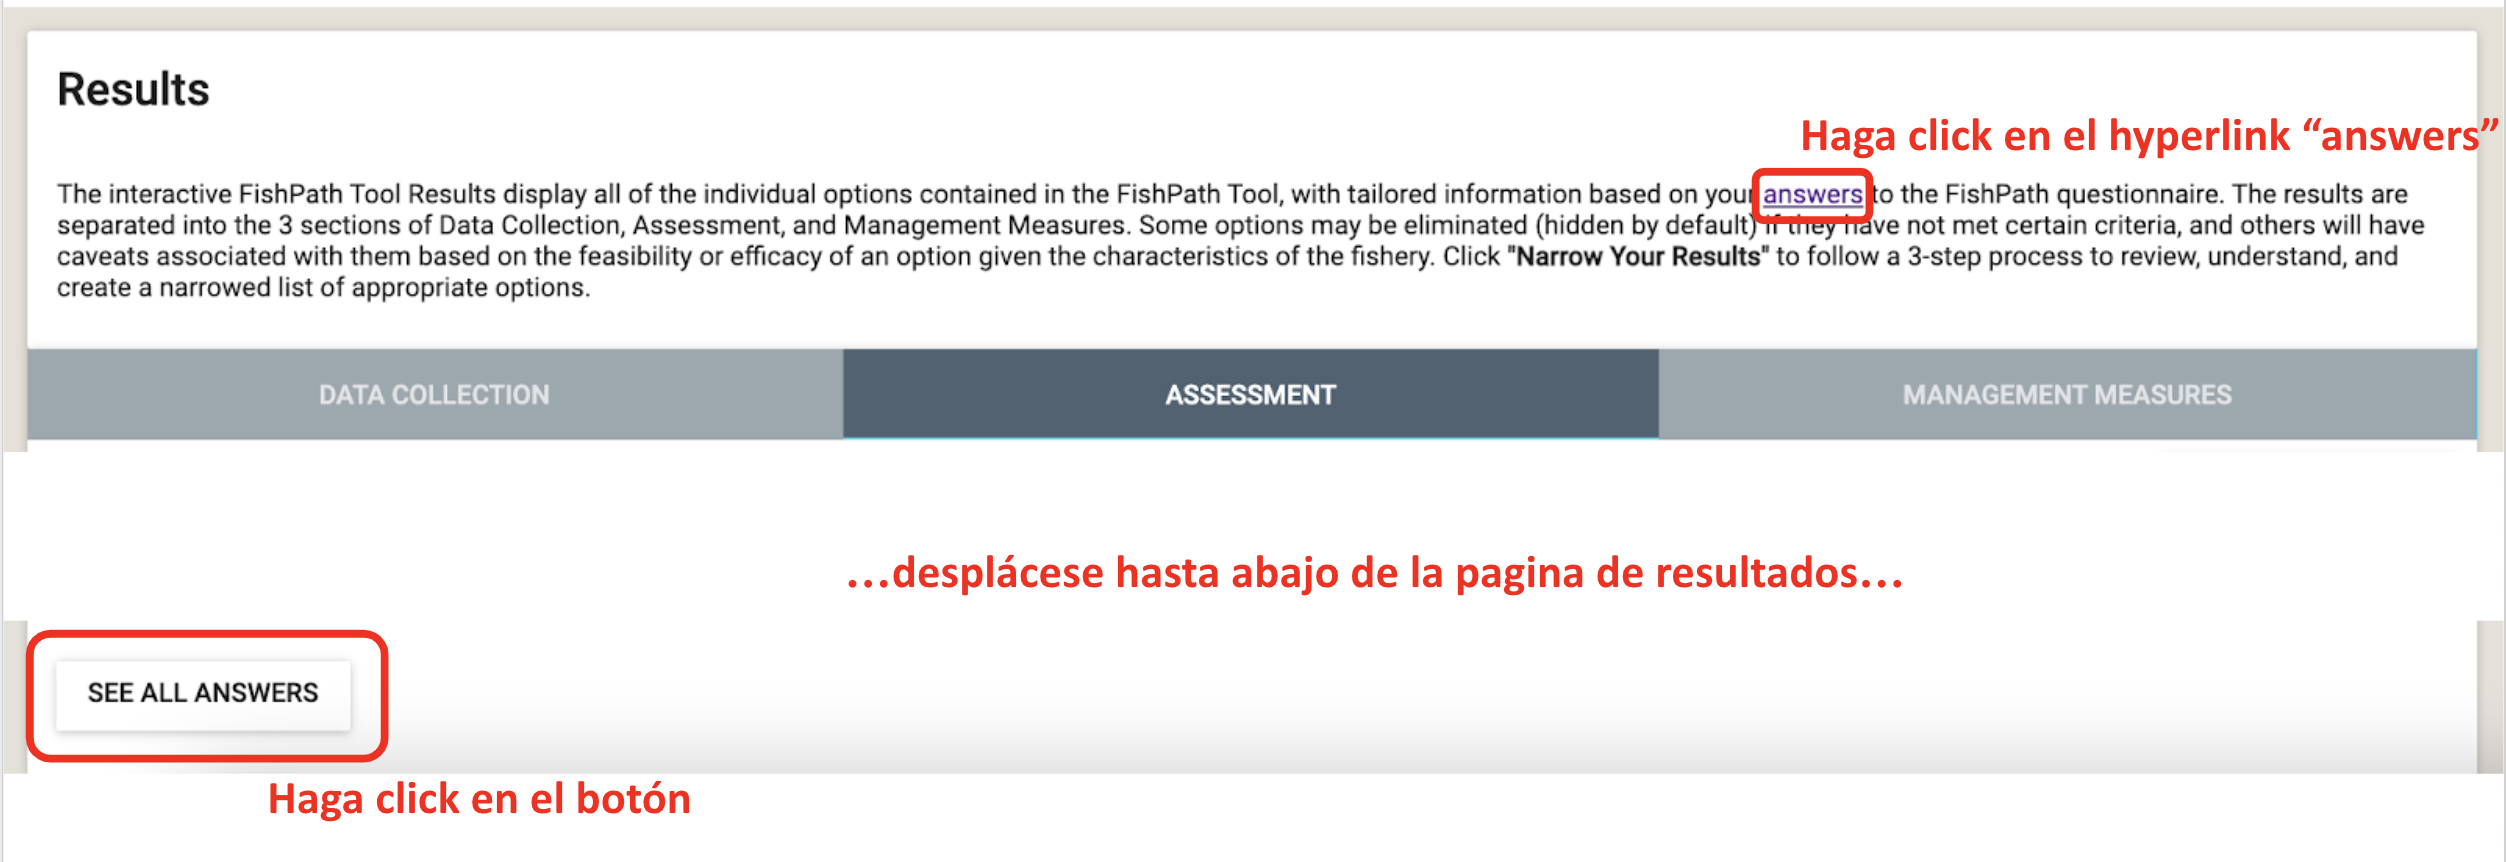
\includegraphics[width=0.75\linewidth]{images/see-all-answers-buttons-es} \caption{Hay dos maneras de ver todas las respuestas al cuestionario en la página de resultados (texto en rojo).}\label{fig:answers-buttons}
\end{figure}

\hypertarget{Results-Narrowing}{%
\section{Proceso para reducir el número de resultados}\label{Results-Narrowing}}

Típicamente, el cuestionario de FishPath da como resultado una larga lista de opciones potenciales que son presentadas al usuario. El desafío para el usuario es el de reducir estas opciones a una lista corta y viable de opciones que pueden ser revisadas a mayor detalle, y alrededor de las cuales se pueda desarrollar una estrategia de capturas. Este puede ser un desafío desalentador, dado el número de las opciones y la gran cantidad de detalles alrededor de los criterios y advertencias.

El proceso para reducir resultados guía al usuario a través de una serie de pasos para refinar y reducir las opciones para su pesquería, y para considerar los detalles de cada opción en la pesquería. \textbf{La meta es obtener una lista corta, justificable, apropiada y bien documentada para la pesquería.}

Primero, el usuario puede acceder al proceso de reducir los resultados al seleccionar ``Reducir tus resultados'' localizado encima de la tabla de resultados en la pantalla de resultados (Ver Figura \ref{fig:results-overview}).

Después de hacer clic en ``Revisar sus resultados'', el usuario es dirigido a un proceso de revisión de resultados (Figura \ref{fig:results-review-header}). Cada paso del proceso de revisión de resultados contiene un cuadro de ``Instrucciones'' con pasos claros, así como la capacidad de acceder a distintos pasos del proceso de revisión de resultados a través de ``Atrás'' (o ``Back''), ``Salir'' (o ``Exit Review'') y ``Paso siguiente'' (o ``Next Step''). La cinta azul en la parte superior de la página muestra en qué paso del proceso se encuentra el usuario.

\begin{figure}

{\centering 
\includegraphics[width=0.95\linewidth]{images/results-review-header} 

}

\caption{Los pasos en el proceso de reducción de resultados.}\label{fig:results-review-header}
\end{figure}

El proceso para reducir resultados (realizado en grupo o de manera individual), consiste de los siguientes pasos:

\begin{enumerate}
\def\labelenumi{\arabic{enumi}.}
\tightlist
\item
  \textbf{Opción para retener (Figure \ref{fig:review-step-1}):} La meta de este primer paso es esconder todas aquellas opciones que claramente no son viables para la pesquería ya que no se cumplieron criterios mínimos y/o debido a razones logísticas de implementación, marco legal o político, etc. Los usuarios deben revisar la lista y esconder estas opciones, así como mostrar las opciones que se escondieron automáticamente y quieran reintegrar. Las instrucciones se muestran en la parte superior de la pantalla en esta parte del proceso, incluyendo algunas preguntas a considerar para reducir la lista. Al terminar, el usuario hace click en el botón de ``Next step'' o ``Próximo paso'' y una palomita azul aparecerá junto a ``Option Retention'' o ``Retención de opciones'' en la banda azul de la parte superior de la pantalla.
\end{enumerate}

\begin{figure}

{\centering 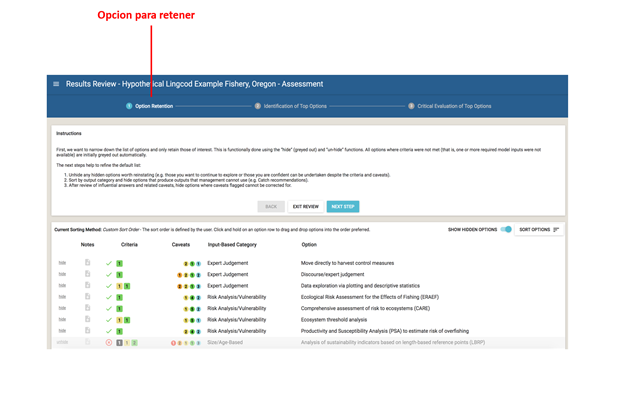
\includegraphics[width=0.95\linewidth]{images/review-step-1-es} 

}

\caption{Paso 1, Retener opciones dentro del proceso para reducir resultados.}\label{fig:review-step-1}
\end{figure}

\begin{enumerate}
\def\labelenumi{\arabic{enumi}.}
\setcounter{enumi}{1}
\tightlist
\item
  \textbf{Identificación de las opciones más apropiadas (Figure \ref{fig:review-step-2}):} En este paso, los usuarios revisan las opciones restantes con el fin de llegar a una lista reducida, más manejable, con las opciones que serán consideradas con mayor seriedad y serán exploradas con mayor detalle. Los usuarios deben familiarizarse con ordenar la lista de características y respuestas influyentes (ver arriba) con el fin de facilitar el proceso. Al comparar opciones, los usuarios deberían de comparar los criterios, advertencias de precaución y su impacto relativo, así como los atributos positivos. Las instrucciones se muestran en la parte superior de la pantalla. Conforme el usuario marca las opciones con una estrella (en la primera columna se tiene la habilidad de marcar las mejores o más apropiadas opciones), un círculo anaranjado aparece junto a este paso en la banda azul de la parte superior de la pantalla. El número que aparece en el círculo representa el número de las opciones que han sido marcadas y una palomita azul aparecerá junto a este paso una vez que el usuario haga click en Next step o ``Próximo paso''.
\end{enumerate}

\begin{figure}

{\centering 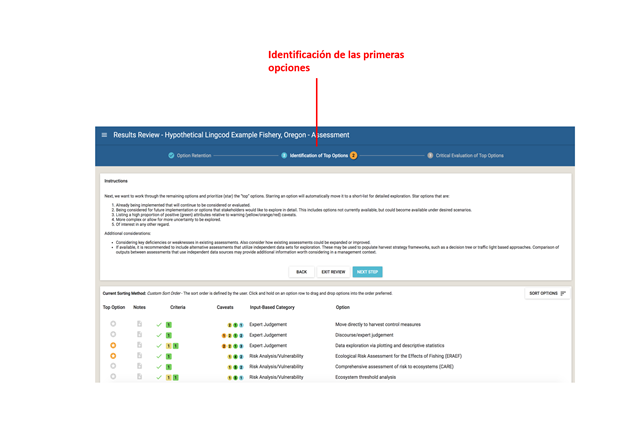
\includegraphics[width=0.95\linewidth]{images/review-step-2-es} 

}

\caption{Paso 2, Identificación de las mejores opciones o las más apropiadas}\label{fig:review-step-2}
\end{figure}

\begin{enumerate}
\def\labelenumi{\arabic{enumi}.}
\setcounter{enumi}{2}
\tightlist
\item
  \textbf{Evaluación critica de las mejores opciones (Figure \ref{fig:review-step-3}):} En el paso tercero y final, los usuarios pueden evaluar de manera mas crítica las opciones al considerar cada uno de sus criterios y advertencias a detalle y potencialmente ranquear las opciones en orden de su viabilidad y potencial de implementación.
\end{enumerate}

\begin{figure}

{\centering 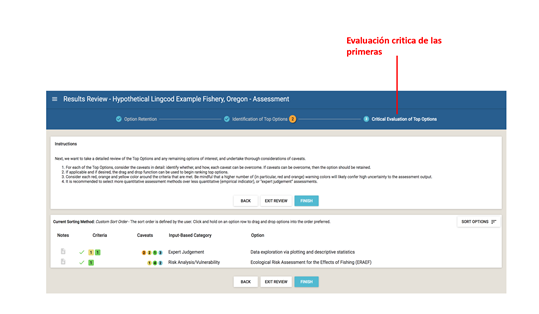
\includegraphics[width=0.95\linewidth]{images/review-step-3-es} 

}

\caption{Paso 3, evaluación crítica de las mejores opciones.}\label{fig:review-step-3}
\end{figure}

Una vez que se completa este paso, los usuarios deben hacer click en ``Finish'' o ``Finalizar'' para regresar a la página de resultados. Los resultados en este momento solamente mostrarán aquellas opciones filtradas o la lista de mejores opciones. Los usuarios pueden alternar entre las opciones reducidas y la lista completa. Los usuarios pueden generar un reporte en PDF de las opciones reducidas al hacer click en el botón de ``Generate PDF Report'' o ``Generar reporte en PDF'' mientras el filtro de la lista de mejores opciones se mantiene.

\hypertarget{Results-Actions}{%
\section{Acciones para compartir resultados y editar información de la pesquería}\label{Results-Actions}}

En la parte superior de la página de resultados, el usuario puede ``Compartir'', ``Exportar documento CSV'', ``Copiar'', ``Generar un reporte PDF'' o ``Editar nombre y detalles'' de los resultados de su pesquería (Figura \ref{fig:results-components}).

\begin{itemize}
\tightlist
\item
  \textbf{Compartir:} Esto generará un link que permite al usuario compartir los resultados de su pesquería con otras personas. El usuario simplemente debe mandar su vínculo o link y con este, el recipiente tendrá \protect\hyperlink{View-Only}{\textbf{acceso a la pesquería únicamente desde su cuenta activa}}. Una pesquería que ha sido compartida puede ser guardada en la cuenta FishPath de otra persona, que puede hacer una copia de dicha pesquería y editarla de manera separada si es necesario. Sugerencia: cuando se genera una copia de una pesquería compartida en la cuenta de un usuario, se recomienda renombrar la pesquería para que los cambios sean guardados bajo este nuevo nombre.
\item
  \textbf{Exportar documento CSV:} Esto permite al usuario exportar la lista de preguntas y respuestas del cuestionario previamente guardado, asi como un documento con los resultados, como un .csv.
\item
  \textbf{Generar reporte PDF:} Permite generar un reporte de los resultados y las notas agregadas en FishPath, en formato .PDF. El reporte provee información detallada de cada opcion, así como sus advertencias y criterios asociados a la pesquería. Los usuarios pueden elegir que el reporte incluya una lista completa o solamente las opciones más apropiadas.
\item
  \textbf{Copiar pesquería:} Esto permite al usuario copiar los resultados de una pesquería, ya sea de su propia cuenta o de un link que fue compartido. El usuario puede actualizar la información de su pesquería, la cual va a ser guardada en su tablero.
\item
  \textbf{Editar nombre y detalles:} Esto permite al usuario editar la información que fue ingresada en la sección de ``información de la pesquería'' (nombre, especie, área geográfica, etc.).
\end{itemize}

\hypertarget{View-Only}{%
\section{Modo de solo visualización (Pesquería compartida)}\label{View-Only}}

Los usuarios pueden \protect\hyperlink{Results-Actions}{\textbf{compartir con otras personas su cuestionario y los resultados}} del mismo al compartir un link, pero las respuestas no pueden ser editadas por otras personas. Esto ayuda a mantener fidelidad de los resultados sin importar cuantas personas vean la pesquería.

Al hacer click en el link compartido, el usuario podrá ver los resultados en modo de ``visualización únicamente'' (Figura \ref{fig:view-only}). En este modo el usuario puede explorar los resultados y respuestas provistas por el usuario original pero no podrá hacer cambios. El usuario puede ordenar y filtrar opciones, sin embargo, la funcionalidad de editar esta deshabilitada, así como la habilidad de actualizar o editar el cuestionario o añadir notas. Las opciones sombreadas en gris indican aquellas opciones que han sido escondidas por el usuario original. Si el usuario original añadió notas, estas aparecerán con un ícono de una nota amarilla en modo de ver únicamente.

El usuario puede ``Copiar la pesquería'', permitiéndole editar detalles de la pesquería como nombre y ubicación, y luego hacer ediciones. Esta pesquería ``copiada'' aparecerá en su tablero.

\begin{figure}

{\centering 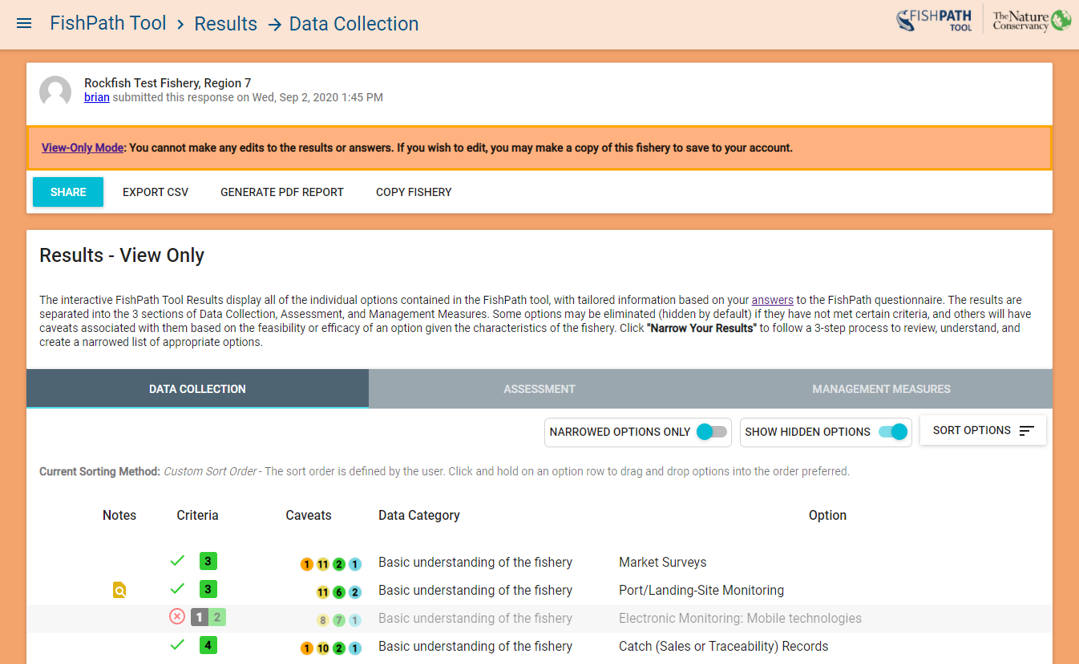
\includegraphics[width=0.95\linewidth]{images/view-only} 

}

\caption{El modo “visualización únicamente” de los resultados de la herramienta FishPath.}\label{fig:view-only}
\end{figure}

\hypertarget{appendix-appendix}{%
\appendix}


\hypertarget{fishpath-tool-frequently-asked-questions-faqs}{%
\chapter{FishPath Tool Frequently Asked Questions (FAQs)}\label{fishpath-tool-frequently-asked-questions-faqs}}

\hypertarget{faq-feedback}{%
\paragraph{How do I submit feedback about content or user experience?}\label{faq-feedback}}

FishPath benefits from the expertise and feedback of the global community of FishPath tool users. Users are encouraged to submit feedback about the FishPath tool, ultimately helping to improve the tool. There are two ways to submit feedback:

\begin{enumerate}
\def\labelenumi{\arabic{enumi}.}
\tightlist
\item
  The ``Submit Feedback'' button on FishPath Tool Dashboard. The user is prompted to categorize their feedback as ``Content Related'' or ``Software Issue''.
\item
  Email \href{mailto:support@fishpath.org}{\nolinkurl{support@fishpath.org}}
\end{enumerate}

\hypertarget{faq-content-updates}{%
\paragraph{How does the FishPath Tool content (questions, options, caveats, etc.) get updated? And how often?}\label{faq-content-updates}}

The FishPath team is composed of practicing fisheries managers and scientists who stay up to date on the changing field of fisheries research. The Tool is maintained with the aim of being as current with fishery management practices, science and literature as possible. We also strive to correct any mistakes found in the Tool as quickly as possible. In order to do this, content updates can be made at any time.

Suggestions from users regarding the content is also greatly appreciated and encouraged. We recognize that fisheries occur in a wide variety of contexts and our small team cannot know every possible scenario and caveat. Any feedback will get a full review and be incorporated into the Tool as needed.

Every time a user logs in, the Tool will use the most up to date version of the Tool content. No action is needed to receive the updates, even if the questionnaire is already completed. If a new question has been added after a user has completed the questionnaire, a prompt will appear to answer that question before returning to the results screen.

\hypertarget{faq-stay-updated}{%
\paragraph{How do I stay updated on changes to the FishPath Tool questionnaire or content?}\label{faq-stay-updated}}

A brief summary of any major changes is documented in the biannual newsletter. A changelog is under development which will document all the changes made after April 2021.

\hypertarget{faq-copy-fisheries}{%
\paragraph{Are answers to new questions also updated in ``copied fisheries''?}\label{faq-copy-fisheries}}

Once a fishery is copied, changes in the original or copied fishery will have no effect on the other.

\hypertarget{faq-internet}{%
\paragraph{Does the FishPath Tool need the internet to run?}\label{faq-internet}}

The FishPath Tool does require an internet connection to load and function properly. However, the Tool has been designed to handle poor or intermittent internet connections. Once logged in, the Tool can partially function without the internet. If the internet cuts out or lags while working, the Tool will store any answers to questions or changes made while offline in the browser until it is able to reconnect with the server and save the changes. The {[}saving status toolbar{]}{[}Saving Status Toolbar{]} across the bottom of the screen lets the user know if any changes have not been able to be saved to the server. Closing the window or navigating away from the Tool when there are unsaved changes, will cause those changes to be lost.

\hypertarget{faq-question-numbering}{%
\paragraph{Why does the number of questions for each section appear to change?}\label{faq-question-numbering}}

Many of the questions in the questionnaire are relevant to multiple sections. Once you answer a question that affects multiple sections, the Tool will not repeat that question again when completing the questionnaire for another section. For example, before starting the questionnaire for any section, there are 41 questions in Data Collection, 50 questions in Assessment, and 44 in Management Measures. A user starts by completing the Data Collection questionnaire. 6 of those questions also apply to Assessment and 14 apply to Management Measures as well. If the user answers the Assessment section next, instead of being asked all 50 questions, only 44 would be asked, since 6 of the questions have already been answered when completing the Data Collection questionnaire. Likewise, if the user answers the Management Measures section next, only 30 questions would be asked.

\hypertarget{terms}{%
\chapter{FishPath Tool Terms of Service}\label{terms}}

\textbf{Last revised on October 23, 2018}

The Nature Conservancy (``TNC,'' ``we,'' ``us,'' or ``our'') are pleased to provide FishPath and related software, data, websites, instructions, and services (``FishPath'') to you. If you are using FishPath on behalf of a business (such as your employer), that business accepts these terms of service (``Terms'') by your use. In that case, the words ``You'' and ``Your'' in these Terms refer to both you and that business.

The Terms govern Your access to and use of FishPath, so please carefully read them and Our Privacy Policy before using FishPath. By registering on the FishPath websites and using FishPath, You agree to be bound by these Terms and by our Privacy Policy. If You don't agree with these Terms and our Privacy Policy, You cannot use FishPath or FishPath data in any way or at any time.

\hypertarget{fishpath-data-your-rights-and-your-privacy}{%
\subsubsection*{FishPath Data: Your Rights and Your Privacy}\label{fishpath-data-your-rights-and-your-privacy}}
\addcontentsline{toc}{subsubsection}{FishPath Data: Your Rights and Your Privacy}

We developed FishPath as a user-friendly application to help users diagnose the challenges in their fishery and select appropriate options for data collection, stock assessment, and management measures. FishPath allows You to use Your fishery information (Your ``Submission''). Your Submission to FishPath is voluntary. If You submit information to FishPath, these Terms do grant us the right to see and use Your Submission to improve the functionality of the tool as appropriate. We may copy and share an anonymized aggregation of information from submissions, potentially including Your Submission, with the public. However, we will not share Your submission nor Your information in any non aggregated format.

Please refer to our \href{https://www.nature.org/en-us/about-us/who-we-are/accountability/privacy-policy/}{Privacy Policy} for a description of how we collect, use and disclose FishPath information, including Your Submission. We have the right to withdraw or change FishPath. As we describe below, we will not be liable to You if for any reason all or any part of FishPath is unavailable at any time or for any length of time.

\hypertarget{your-responsibilities}{%
\subsubsection*{Your Responsibilities}\label{your-responsibilities}}
\addcontentsline{toc}{subsubsection}{Your Responsibilities}

Only make a Submission if You have all necessary rights to share the information with us, including but not limited to use with FishPath. You are solely responsible for your conduct and Your Submission while using FishPath. It is Your responsibility to ensure that You have the rights or permission needed to comply with these Terms.

Respect the law. Do not use FishPath for any fraudulent or unlawful purpose including violations of statutory, regulatory or contractual law. Respect copyright, privacy, trade secret, data protection, fish \& wildlife and all other laws. Do not attempt to impersonate any other individual on FishPath; if You identify yourself, You must always use Your true identity.

Without our express written consent, You may not use, display, mirror, or frame FishPath, any element within FishPath, or any proprietary elements belonging to us (including but not limited to our logos and marks). In addition to adhering to all applicable laws and regulations, You may NOT do any of the following:

\begin{itemize}
\tightlist
\item
  resell FishPath or data from FishPath, or any portion thereof;
\item
  access or search the FishPath data by using any engine, software, tool, agent, device or mechanism (including spiders, robots, crawlers, data mining tools or the like) other than the software and/or search agents that We provide or authorize;
\item
  probe, scan, tamper with, or test the vulnerability of FishPath or any of our systems or networks;
\item
  avoid, breach, deactivate, impair, or circumvent any security or authentication measures, including those that protect FishPath and its data;
\item
  attempt to decipher, decompile, disassemble or reverse engineer any of the software used to provide FishPath;
\item
  interfere with, or attempt to interfere with, the access of any user, host or network, including, without limitation, by sending a virus, overloading, or flooding FishPath;
\item
  encourage or enable anyone else to do any of the foregoing.
\end{itemize}

We have the right to investigate violations of these Terms or conduct that affect FishPath or our systems or networks. We may also consult and cooperate with law enforcement authorities to prosecute users who violate the law.

\hypertarget{rights-you-grant-in-your-information}{%
\subsubsection*{Rights You Grant in Your Information}\label{rights-you-grant-in-your-information}}
\addcontentsline{toc}{subsubsection}{Rights You Grant in Your Information}

By making Your Submission, You grant us a non-exclusive, transferable, sublicensable, worldwide, perpetual, royalty-free license to use, copy, modify, create derivative works based upon, distribute, publicly display, publicly perform and distribute Your Submission. We will not, however, share or distribute specific notes You submit for Your fishery.

\hypertarget{rights-that-we-grant-you}{%
\subsubsection*{Rights That We Grant You}\label{rights-that-we-grant-you}}
\addcontentsline{toc}{subsubsection}{Rights That We Grant You}

Subject to Your compliance with these Terms, we grant You a limited, non-exclusive, non-transferable, non-sublicensable, worldwide, royalty-free license to use the FishPath software, instructions, and websites and to view, copy, display, and create derivative works from the FishPath output that we make available from the FishPath site for Your management of Your fishery.

You may not: (i) copy, modify or create derivative works based on the FishPath software; (ii) distribute, transfer, sublicense, lease, or rent the FishPath software to any third party; or (iii) reverse engineer, decompile or disassemble the FishPath software.

Using FishPath or uploading Data does not give You ownership of any intellectual property rights in FishPath (other than your own Submission). We and our licensors exclusively own all right, title and interest in and to FishPath, including all associated intellectual property rights. You acknowledge that copyright, trademark, and other laws of the United States and foreign countries protect FishPath. You agree not to remove, alter or obscure any copyright, trademark, service mark or other proprietary rights notices incorporated in or accompanying FishPath.

These Terms do not grant You the right to use any of our branding or logos or names. You must not use our names or logos or branding without our written permission.

\hypertarget{modifying-our-terms-of-service}{%
\subsubsection*{Modifying our Terms of Service}\label{modifying-our-terms-of-service}}
\addcontentsline{toc}{subsubsection}{Modifying our Terms of Service}

We may update these Terms from time to time, in our sole discretion. We may notify You of such updates by any reasonable means, such as by posting the revised Terms on the FishPath website. Please look at the ``LAST UPDATED'' legend above to see when these Terms were last revised. Your use of FishPath after the posting of any revised Terms means that You accept and agree to be bound by the revised Terms. If You don't agree to be bound by the revised Terms, then You may not use FishPath anymore. You can stop using FishPath at any time. We may also stop providing FishPath or add or create new limits to FishPath at any time.

\hypertarget{disclaimers-limited-liability-and-indemnity}{%
\subsubsection*{Disclaimers, Limited Liability and Indemnity}\label{disclaimers-limited-liability-and-indemnity}}
\addcontentsline{toc}{subsubsection}{Disclaimers, Limited Liability and Indemnity}

As we describe in more detail below, FishPath and its data are a general information resource and are provided solely ``AS IS'' and ``AS AVAILABLE'' without warranty of any kind. You should not construe publication of FishPath data as a warranty or guarantee of the quality or availability of any goods or services or technical support.

\hypertarget{disclaimers-and-limitation-of-liability}{%
\subsubsection*{DISCLAIMERS AND LIMITATION OF LIABILITY}\label{disclaimers-and-limitation-of-liability}}
\addcontentsline{toc}{subsubsection}{DISCLAIMERS AND LIMITATION OF LIABILITY}

ALL CONTENT ON FISHPATH IS PROVIDED ``AS IS'' AND ``AS AVAILABLE'' WITHOUT WARRANTY OF ANY KIND, EITHER EXPRESS OR IMPLIED. WITHOUT LIMITING THE FOREGOING, WE EXPLICITLY DISCLAIM ANY AND ALL WARRANTIES OF MERCHANTABILITY, FITNESS FOR A PARTICULAR PURPOSE, QUIET ENJOYMENT, OR NON-INFRINGEMENT, AND ANY AND ALL WARRANTIES ARISING OUT OF COURSE OF DEALING OR USAGE OF TRADE. TNC MAKES NO WARRANTY AS TO THE QUALITY, ACCURACY, COMPLETENESS, TIMELINESS, OR RELIABILITY OF FISHPATH OR ANY FISHPATH CONTENT. YOUR USE OF FISHPATH IS AT YOUR SOLE RISK.

TNC MAKES NO REPRESENTATIONS OR WARRANTIES THAT YOUR USE OF FISHPATH WILL MEET YOUR NEEDS OR BE UNINTERRUPTED, SECURE, OR ERROR FREE. USERS ARE RESPONSIBLE FOR TAKING ALL NECESSARY PRECAUTIONS TO ENSURE THAT ANY CONTENT YOU MAY OBTAIN FROM THE SERVICES IS FREE OF VIRUSES OR OTHER HARMFUL CODE.

TO THE MAXIMUM EXTENT PERMITTED BY LAW, WE SHALL NOT BE LIABLE FOR CREATING, PRODUCING, MAINTAINING, OPERATING, OR PROVIDING FISHPATH OR FISHPATH CONTENT, UNDER ANY THEORY BASED IN CONTRACT, WARRANTY, TORT (INCLUDING NEGLIGENCE), PRODUCT LIABILITY, STRICT LIABILITY, OR OTHER LEGAL THEORY. THIS LIMITATION ON LIABILITY INCLUDES ANY AND ALL INDIRECT, INCIDENTAL, SPECIAL, EXEMPLARY OR CONSEQUENTIAL DAMAGES, INCLUDING LOST PROFITS, LOSS OF DATA OR GOODWILL, SERVICE INTERRUPTION, COMPUTER DAMAGE OR SYSTEM FAILURE OR THE COST OF SUBSTITUTE SERVICES ARISING OUT OF OR IN CONNECTION WITH THESE TERMS OR FROM THE USE OF OR INABILITY TO USE FISHPATH, EVEN IF WE HAVE BEEN ADVISED OF THE POSSIBILITY OF SUCH DAMAGES.

THE ABOVE EXCLUSIONS AND LIMITATIONS OF DAMAGES ARE FUNDAMENTAL ELEMENTS OF THE BASIS OF THE BARGAIN BETWEEN YOU AND US.

\hypertarget{indemnity}{%
\subsubsection*{Indemnity}\label{indemnity}}
\addcontentsline{toc}{subsubsection}{Indemnity}

You agree to release, indemnify, defend and hold harmless TNC, our subsidiaries and affiliates, and our and their respective officers, directors, agents, partners and employees, from and against any claims, disputes, demands, liabilities, damages, losses, and costs and expenses, including, without limitation, reasonable legal and accounting fees arising out of or in any way connected with (i) Your access to or use of FishPath, (ii) Your Submission, or (iii) Your violation of these Terms.

\hypertarget{termination}{%
\subsubsection*{Termination}\label{termination}}
\addcontentsline{toc}{subsubsection}{Termination}

We may terminate Your access to and use of FishPath, at our sole discretion, at any time and without notice to You. Upon any termination, discontinuation or cancellation of FishPath, all provisions of these Terms that by their nature should survive will survive. This includes, for example ownership provisions, warranty disclaimers, and limitations of liability.

\hypertarget{general-terms}{%
\subsubsection*{General Terms}\label{general-terms}}
\addcontentsline{toc}{subsubsection}{General Terms}

These Terms are the entire and exclusive agreement between You and us regarding FishPath, and they supersede any prior agreements between You and us regarding FishPath.

These terms do not create any third party beneficiary rights. You may not assign or transfer these Terms, by operation of law or otherwise, without our prior written consent. Subject to the foregoing, these Terms will bind your successors and permitted assigns. We may freely assign or transfer these Terms without restriction.

If You do not comply with these Terms, and we do not take action right away, this does not mean that we are giving up any rights that we may have to take action in the future or seek all available remedies.

If it turns out that a particular provision of these Terms is not fully valid or enforceable, that provision will be enforced to the maximum extent permissible, and this will not affect any other Terms.

All claims arising out of this Agreement or relating to FishPath will be governed by the laws of the State of California, excluding the application of its conflicts of law rules. Any legal action or proceeding arising out of this Agreement or relating to these Services shall be brought exclusively in a state or federal court in or for San Francisco, California. You agree that any and all disputes, claims and causes of action arising out of, or connected with these Terms or Your Submission shall be resolved individually, without resort to any form of class action.

\hypertarget{glossary}{%
\chapter{Glossary}\label{glossary}}





Note: The \href{http://www.fao.org/fishery/glossary/en}{FAO Term Portal - Fisheries} has some of the definitions in multiple languages.

\hypertarget{absolute-abundance}{%
\subsection{Absolute Abundance}\label{absolute-abundance}}

The total number of a kind of fish in a population; this is rarely known, and usually estimated from the relative abundance.

Source: \href{https://repository.library.noaa.gov/view/noaa/12856}{Blackhart, K., Stanton, D. G., \& Shimada, A. M. (2006). \emph{NOAA fisheries glossary.} United States Department of Commerce, National Oceanic and Atmospheric Administration.}

\hypertarget{b0-virgin-biomass}{%
\subsection{B0 (Virgin Biomass)}\label{b0-virgin-biomass}}

``B0'', or virgin biomass, refers to the average biomass of a stock that has yet not been fished. It is generally calculated as the long-term average biomass value expected in the absence of fishing mortality. In production models, B0 is also known as carrying capacity. It is often used as a reference value to assist the relative health of a stock, monitoring changes in the ratio between current and virgin biomass (B/B0).

Source: Restrepo V. (1999): Annotated Glossary of Terms in Executive Summary Reports of the International Commission for the Conservation of Atlantic Tunas' Standing Committee on Research and Statistics (SCRS), \emph{ICCAT}.

via \href{http://www.fao.org/fishery/glossary/en}{FAO Term Portal - Fisheries}

\hypertarget{bias}{%
\subsection{Bias}\label{bias}}

An effect which deprives a statistical result of representativeness by systematically distorting it, as distinct from a random error which may distort on any one occasion but balances out on the average.

Source: \href{https://stats.oecd.org/glossary/detail.asp?ID=3605}{OECD Glossary}

\hypertarget{biological-overfishing}{%
\subsection{Biological Overfishing}\label{biological-overfishing}}

Catching such a high proportion of one or all age classes in a fishery as to reduce yields and drive stock biomass, and spawning potential below safe levels. Can involve both growth overfishing and recruitment overfishing. With reference to a surplus production model, biological overfishing occurs when fishing levels are higher that those required for extracting the maximum sustainable yield (MSY) of a resource.

Source: Garcia, S.M. (Comp.). 2009. Glossary. In Cochrane, K. and S.M. Garcia. (Eds). \emph{A fishery manager's guidebook}. FAO and Wiley-Blackwell:473-505.

via \href{http://www.fao.org/fishery/glossary/en}{FAO Term Portal - Fisheries}

\hypertarget{boom-and-bust-population-cycle}{%
\subsection{Boom and Bust Population Cycle}\label{boom-and-bust-population-cycle}}

Species that follow boom-and-bust cycles display high volatility in their population dynamics. This means that their availability is sudden, extreme, and unpredictable.

Source: FishPath Team

\hypertarget{bycatch}{%
\subsection{Bycatch}\label{bycatch}}

Part of a catch of a fishing unit taken incidentally in addition to the target species towards which fishing effort is directed. Some or all of it may be returned to the sea as discards, usually dead or dying

Source: Modified from FAO (1998): Guidelines for the routine collection of capture fishery data

via \href{http://www.fao.org/fishery/glossary/en}{FAO Term Portal - Fisheries}

\hypertarget{capital-stuffing}{%
\subsection{Capital Stuffing}\label{capital-stuffing}}

Costly investments in vessel or gear improvements, to outcompete others for a larger share of available fish. This often leads to higher levels of catch than those intended by managers.

Source: Townsend, R. E. (1985). On capital-stuffing in regulated fisheries. \emph{Land
Economics, 61}(2), 195. \url{https://doi.org/10.2307/3145812}

via Anderson CM, Krigbaum MJ,
Arostegui MC, et al.~How commercial fishing effort is managed. \emph{Fish Fish}. 2018;00:1--18. \url{https://doi.org/10.1111/faf.12339}

\hypertarget{carrying-capacity-k}{%
\subsection{Carrying Capacity (K)}\label{carrying-capacity-k}}

The maximum population of a species that a specific ecosystem can support indefinitely without deterioration of the character and quality of the resource. It represents the point of balance between reproduction potential and environmental constraints.

Source: Scialabba N. (ed.), 1998. \emph{Integrated Coastal Area Management and Agriculture, Forestry and Fisheries}. FAO Guidelines, 256p.

via \href{http://www.fao.org/fishery/glossary/en}{FAO Term Portal - Fisheries}

\hypertarget{catch-per-unit-effort-cpue}{%
\subsection{Catch-Per-Unit-Effort (CPUE)}\label{catch-per-unit-effort-cpue}}

Catch-per-unit-effort (CPUE) is the quantity of fish caught (in number or in weight) with one standard unit of fishing effort; e.g.~number of fish taken per 1,000 hooks per day or weight of fish, in tons, taken per hour of trawling. CPUE is often considered an index of fish biomass (or abundance). CPUE is sometimes referred to as catch rate, and may be used as a measure of economic efficiency of fishing as well as an index of fish abundance.

Source: Modified from FAO (1998a): Guidelines for the routine collection of capture fishery data. \emph{FAO Fisheries Technical Paper.} No.~382. Rome, FAO. 113p.

via \href{http://www.fao.org/fishery/glossary/en}{FAO Term Portal - Fisheries}

\hypertarget{decision-rule}{%
\subsection{Decision Rule}\label{decision-rule}}

See \protect\hyperlink{harvest-control-rule-hcr}{Harvest Control Rule (HCR)}

\hypertarget{determinate-growth}{%
\subsection{Determinate Growth}\label{determinate-growth}}

Determinate growth means that the species does not grow indefinitely. The species stops growing once reaching a final adult stage.

Source: FishPath Team

\hypertarget{economic-overfishing}{%
\subsection{Economic Overfishing}\label{economic-overfishing}}

Occurs when a fishery is generating no economic rent, primarily because an excessive level of fishing effort is applied in the fishery and does not always imply biological overfishing.

Source: FAO Fisheries and Aquaculture Department, FAO, 2014.

via \href{http://www.fao.org/fishery/glossary/en}{FAO Term Portal - Fisheries}

\hypertarget{ecosystem-overfishing}{%
\subsection{Ecosystem Overfishing}\label{ecosystem-overfishing}}

Occurs when the historical species balance (composition and dominance) is significantly modified by fishing (e.g.~with reductions of large, long-lived, demersal predators and increases of small, short-lived species at lower trophic levels).

Source: FAO Fisheries and Aquaculture Department, FAO, 2014.

via \href{http://www.fao.org/fishery/glossary/en}{FAO Term Portal - Fisheries}

\hypertarget{effort-creep}{%
\subsection{Effort Creep}\label{effort-creep}}

Effort creep refers to an increase in effort effectiveness owing to technological progress. These progressions increase the productivity of fishing power, therefore increasing the effective effort. For example, although the number of vessels may be regulated, an increasing number of hooks per vessel or increasing vessel fuel efficiency may demonstrate effort creep.

Source: Squires, Dale, et al.~``Effort rights in fisheries management: general principles and case studies from around the world.'' \emph{Effort rights in fisheries management: General principles and case studies from around the world}. Food and Agriculture Organization of the United Nations, 2016.

\hypertarget{equilibrium}{%
\subsection{Equilibrium}\label{equilibrium}}

In population ecology, equilibrium refers to a state of balance.

Source: FishPath Team

\hypertarget{fecundity}{%
\subsection{Fecundity}\label{fecundity}}

Fecundity is the potential reproductive capacity of an organism or population expressed in the number of eggs (or offspring) produced during each reproductive cycle. Fecundity usually increases with age and size.

Source: \href{https://repository.library.noaa.gov/view/noaa/12856}{Blackhart, K., Stanton, D. G., \& Shimada, A. M. (2006). \emph{NOAA fisheries glossary.} United States Department of Commerce, National Oceanic and Atmospheric Administration.}

\hypertarget{fishery}{%
\subsection{Fishery}\label{fishery}}

A unit determined by an authority or other entity that is engaged in raising and/or harvesting fish. Typically, the unit is defined in terms of some or all of the following: people involved, species or type of fish, area of water or seabed, method of fishing, class of boats and purpose of the activities.

Source: Fletcher, W.J., Chesson, J. Fisher, M., Sainsbury K.J., Hundloe, T. Smith A.D.M., and B. Whitworth (2002): National ESD reporting framework for Australian fisheries: The ``How To'' guide for wild capture fisheries. FRDC Project 2000/145. Canberra, Australia

via \href{http://www.fao.org/fishery/glossary/en}{FAO Term Portal - Fisheries}

\hypertarget{fishery-dependent-data}{%
\subsection{Fishery-Dependent Data}\label{fishery-dependent-data}}

Data collected directly on a fish or fishery from commercial or sport fishermen and seafood dealers. Common methods include logbooks, trip tickets, port sampling, fishery observers, and phone surveys.

Source: \href{https://repository.library.noaa.gov/view/noaa/12856}{Blackhart, K., Stanton, D. G., \& Shimada, A. M. (2006). \emph{NOAA fisheries glossary.} United States Department of Commerce, National Oceanic and Atmospheric Administration.}

\hypertarget{fishery-independent-data}{%
\subsection{Fishery-Independent Data}\label{fishery-independent-data}}

Characteristic of information (e.g.~stock abundance index) or an activity (e.g.~research vessel survey) obtained or undertaken independently of the activity of the fishing sector. Intended to avoid the biases inherent to fishery-related data.

Source: \href{https://repository.library.noaa.gov/view/noaa/12856}{Blackhart, K., Stanton, D. G., \& Shimada, A. M. (2006). \emph{NOAA fisheries glossary.} United States Department of Commerce, National Oceanic and Atmospheric Administration.}

\hypertarget{fishery-effort}{%
\subsection{Fishery Effort}\label{fishery-effort}}

The amount of fishing gear of a specific type used on the fishing grounds over a given unit of time for example hours trawled per day, number of hooks set per day or number of hauls of a beach seine per day. When two or more kinds of gear are used, the respective efforts must be adjusted to some standard type before being added.

Source: FAO. 1997. \emph{Fisheries management}. FAO Technical Guidelines for Responsible Fisheries No.~4. Rome, FAO. 82p.

via \href{http://www.fao.org/fishery/glossary/en}{FAO Term Portal - Fisheries}

\hypertarget{fishing-mortality-f}{%
\subsection{Fishing Mortality (F)}\label{fishing-mortality-f}}

The instantaneous rate of fish deaths due to fishing a component of the fish stock. F reference points may be applied to entire stocks or segments of the stocks.

Source: \url{https://www.fish.gov.au/about/glossary}

\hypertarget{growth-overfishing}{%
\subsection{Growth Overfishing}\label{growth-overfishing}}

Occurs when too many small fish are being harvested too early, through excessive fishing effort and poor selectivity (e.g.~too small mesh sizes) and the fish are not given enough time to grow to the size at which the maximum yield-per-recruit from the stock would be obtained. A reduction of fishing mortality on juveniles, or their outright protection, would lead to an increase in yield from the fishery. Growth overfishing, by itself, does not affect the ability of a fish population to replace itself.

Source: FAO Fisheries and Aquaculture Department, FAO, 2014.

via \href{http://www.fao.org/fishery/glossary/en}{FAO Term Portal - Fisheries}

\hypertarget{harvest-control-rule-hcr}{%
\subsection{Harvest Control Rule (HCR)}\label{harvest-control-rule-hcr}}

Also ``decision rule''. A formally defined, usually quantitative rule, that is used to adjust a management measure in reponse to some known or inferred status of the fished stock. The strength of adjustment of the management measure is usually some function of a performance measure - that is, the proximity of a performance indicator to a target or limit reference point.

Source: FishPath Team

\hypertarget{harvest-strategy}{%
\subsection{Harvest Strategy}\label{harvest-strategy}}

Also ``management strategy''. A harvest (or management) strategy is a formal, pre-specified set of rules designed to achieve the management objectives for the fishery. Harvest strategies (HSs) are formal frameworks for managing exploitation of fisheries, usually applied to the target species (e.g.~Sainsbury et al.~2000, Butterworth and Punt 2003). They comprise a fully-specified set of rules for making tactical management decisions including specifications for i) a monitoring (data collection) program, ii) the indicators to be calculated from monitoring data (usually via a stock assessment) and iii) the use of those indicators and their associated reference points in management decisions, through application of decision (or control) rules.

Sources: Butterworth, D.S., and Punt, A.E. 2003. The role of harvest control laws, risk and uncertainty and the precautionary approach in ecosystem-based management. \emph{Responsible Fisheries in the Marine Ecosystem}: 311-319.

Sainsbury, K.J., Punt, A.E., and Smith, A.D.M. 2000. Design of operational management strategies
for achieving fishery ecosystem objectives. \emph{ICES Journal of Marine Science} 57: 731-741.

\hypertarget{illegal-unregulated-and-unreported-iuu-fishing}{%
\subsection{Illegal, unregulated, and unreported (IUU) Fishing}\label{illegal-unregulated-and-unreported-iuu-fishing}}

Reference to broad activities classified as illegal, unreported and unregulated fishing are included in the IPOA-IUU as follows:

\emph{Illegal fishing}:

-conducted by national or foreign vessels in waters under the jurisdiction of a State, without the permission of that State, or in contravention of its laws and regulations;
-conducted by vessels flying the flag of States that are parties to a relevant regional fisheries management organisation but operate in contravention of the conservation and management measures adopted by that organisation and by which the States are bound, or relevant provisions of the applicable international law; or
-in violation of national laws or international obligations, including those undertaken by cooperating States to a relevant regional fisheries management organization.

\emph{Unreported fishing}:

-which have not been reported, or have been misreported, to the relevant national authority, in contravention of national laws and regulations; or
-are undertaken in the area of competence of a relevant regional fisheries management organisation which have not been reported or have been misreported, in contravention of the reporting procedures of that organisation.

\emph{Unregulated fishing}:

-in the area of application of a relevant regional fisheries management organization that are conducted by vessels without nationality, or by those flying the flag of a State not party to that organization, or by a fishing entity, in a manner that is not consistent with or contravenes the conservation and management measures of that organization; or
-in areas or for fish stocks in relation to which there are no applicable conservation or management measures and where such fishing activities are conducted in a manner inconsistent with State responsibilities for the conservation of living marine resources under international law.

Source: \url{http://www.fao.org/iuu-fishing/background/what-is-iuu-fishing/en/}

\hypertarget{indicators}{%
\subsection{Indicators}\label{indicators}}

A variable, pointer, or index. Its fluctuation reveals the variations in key elements of a system. The position and trend of the indicator in relation to reference points or values indicate the present state and dynamics of the system. Indicators provide a bridge between objectives and action.

Source: FAO (1999): Indicators for sustainable development of marine capture fisheries. \emph{FAO Technical Guidelines for Responsible Fisheries}, 8: 68 p.~Rome, FAO

via \href{http://www.fao.org/fishery/glossary/en}{FAO Term Portal - Fisheries}

\hypertarget{intrinsic-growth-rate-r}{%
\subsection{Intrinsic growth rate (r)}\label{intrinsic-growth-rate-r}}

A value that quantifies how much a population can grow between successive time periods. The intrinsic growth rate is often estimated with production models and plays an important role in evaluating the sustainability of different harvest levels and the capacity to recover after depletion.

Source: Restrepo V. (1999): Annotated Glossary of Terms in Executive Summary Reports of the International Commission for the Conservation of Atlantic Tunas Standing Committee on Research and Statistics (SCRS). \emph{ICCAT}.

via \href{http://www.fao.org/fishery/glossary/en}{FAO Term Portal - Fisheries}

\hypertarget{latent-effort}{%
\subsection{Latent effort}\label{latent-effort}}

Fishing capacity that is authorised for use but not currently being used. Depending on how a fishery is managed, latency might appear in effort (for example, unused vessel statutory fishing rights {[}SFRs{]}, gear SFRs, quota SFRs, permits or nights fishing) or in quota (for example, where total allowable catches {[}TACs{]} are not fully caught in a quota-managed fishery). It can be an indicator of fishers' views about the profitability of a fishery, with high levels of latency suggesting that low expected profits in the fishery do not justify fishing.

Source: \url{https://www.fish.gov.au/about/glossary}

\hypertarget{length-weight-relationship}{%
\subsection{Length-weight relationship}\label{length-weight-relationship}}

A mathematical formula for calculating the weight of a fi sh in terms of its length. When only one is known, the formula can determine the other

Source: \href{https://repository.library.noaa.gov/view/noaa/12856}{Blackhart, K., Stanton, D. G., \& Shimada, A. M. (2006). \emph{NOAA fisheries glossary.} United States Department of Commerce, National Oceanic and Atmospheric Administration.}

\hypertarget{limit-reference-point}{%
\subsection{Limit reference point}\label{limit-reference-point}}

Indicates the limit beyond which the state of a fishery and / or a resource is not considered desirable. Fishery development should be stopped before reaching it. If a LRP is inadvertently reached, management action should severely curtail or stop fishery development, as appropriate, and corrective action should be taken.

Source: Garcia S.M. (1996)The precautionary approach to fisheries and its implications for fishery research, technology and management: An updated review. \emph{FAO Fisheries Technical Paper}, 350.2: 1-76

via \href{http://www.fao.org/fishery/glossary/en}{FAO Term Portal - Fisheries}

\hypertarget{management-strategy}{%
\subsection{Management Strategy}\label{management-strategy}}

See \protect\hyperlink{harvest-strategy}{Harvest Strategy}

\hypertarget{maturity-ogive}{%
\subsection{Maturity ogive}\label{maturity-ogive}}

The curve resulting from the proportion of mature fish at a given size or length.

Source: FishPath Team

\hypertarget{maximum-sustainable-yield-msy}{%
\subsection{Maximum sustainable yield (MSY)}\label{maximum-sustainable-yield-msy}}

The highest theoretical equilibrium yield that can be continuously taken (on average) from a stock under existing (average) environmental conditions without affecting significantly the reproduction process.

Source: FAO Fisheries and Aquaculture Department, FAO, 2014.

via \href{http://www.fao.org/fishery/glossary/en}{FAO Term Portal - Fisheries}

\hypertarget{multispecies-fishery}{%
\subsection{Multispecies fishery}\label{multispecies-fishery}}

A multispecies fishery is a fishery in which more than one species is caught at the same time. Because of the imperfect selectivity of most fi shing gears, most fisheries are ``multispecies.'' The term is often used to refer to fisheries where more than one species is intentially sought and retained.

Source: \href{https://repository.library.noaa.gov/view/noaa/12856}{Blackhart, K., Stanton, D. G., \& Shimada, A. M. (2006). \emph{NOAA fisheries glossary.} United States Department of Commerce, National Oceanic and Atmospheric Administration.}

\hypertarget{natural-mortality-m}{%
\subsection{Natural mortality (M)}\label{natural-mortality-m}}

Deaths of fish from all causes except fishing (e.g.~ageing, predation , cannibalism, disease and perhaps increasingly pollution). It is often expressed as a rate that indicates the percentage of fish dying in a year; for example a natural mortality rate of 0.2 implies that approximately 20\% of the population will die in a year from causes other than fishing.

Source: FAO Fisheries and Aquaculture Department, FAO, 2014.

via \href{http://www.fao.org/fishery/glossary/en}{FAO Term Portal - Fisheries}

\hypertarget{no-take-reserve}{%
\subsection{No-take reserve}\label{no-take-reserve}}

Areas where extractive activities are prohibited

Sala, E., and Giakoumi, S. 2017. No-take marine reserves are the most effective protected areas in the ocean. -- ICES Journal of Marine Science, 75: 1166--1168.

\hypertarget{nursery}{%
\subsection{Nursery}\label{nursery}}

Nursery refers to the part of a fish's or animal's habitat where the young develop and grow.

Source: \href{https://repository.library.noaa.gov/view/noaa/12856}{Blackhart, K., Stanton, D. G., \& Shimada, A. M. (2006). \emph{NOAA fisheries glossary.} United States Department of Commerce, National Oceanic and Atmospheric Administration.}

\hypertarget{open-access}{%
\subsection{Open Access}\label{open-access}}

Any fishery that does not limit effort or inclusion in the fishery. A fishery without permits or one with unlimited permits are both examples of an open access fishery.

Source: FishPath Team

\hypertarget{overfished}{%
\subsection{Overfished}\label{overfished}}

A stock is considered overfished when exploited beyond an explicit limit beyond which its abundance is considered ``too low'' to ensure safe reproduction. In many fisheries fora the term is used when biomass has been estimated to be below a limit biological reference point that is used as the signpost defining an ``overfished condition''.

Source: Mace, P.M. 1998. The status of ICCAT species relative to optimum yield and overfishing criteria recently proposed in the United States, also with consideration of the precautionary approach. \emph{ICCAT} SCRS/97/074.

via \href{http://www.fao.org/fishery/glossary/en}{FAO Term Portal - Fisheries}

\hypertarget{overfishing}{%
\subsection{Overfishing}\label{overfishing}}

A generic term used to refer to the state of a stock subject to a level of fishing effort or fishing mortality such that a reduction of effort would, in the medium term, lead to an increase in the total catch. Often referred to as overexploitation and equated to biological overfishing, it results from a combination of growth overfishing and recruitment overfishing and occurs often together with ecosystem overfishing and economic overfishing.

Source: Garcia, S.M. (Comp.). 2009. Glossary. In Cochrane, K. and S.M. Garcia. (Eds). \emph{A fishery manager's guidebook}. FAO and Wiley-Blackwell:473-505.

via \href{http://www.fao.org/fishery/glossary/en}{FAO Term Portal - Fisheries}

\hypertarget{periodic-strategist}{%
\subsection{Periodic strategist}\label{periodic-strategist}}

Periodic strategists are characterized by large body size, late maturation, high fecundity, and low juvenile survivorship and are likely to be favored in highly periodic (seasonal) environments

Source: Mims, M.C. and Olden, J.D., 2012. Life history theory predicts fish assemblage response to hydrologic regimes. \emph{Ecology}, 93(1), pp.35-45.

\hypertarget{recruitment}{%
\subsection{Recruitment}\label{recruitment}}

The number of fish added to the exploitable stock, in the fishing area, each year, through a process of growth (i.e.~the fish grows to a size where it becomes catchable) or migration (i.e.~the fish moves into the fishing area).

Source: Garcia, S.M. (Comp.). 2009. Glossary. In Cochrane, K. and S.M. Garcia. (Eds). \emph{A fishery manager's guidebook}. FAO and Wiley-Blackwell:473-505.

via \href{http://www.fao.org/fishery/glossary/en}{FAO Term Portal - Fisheries}

\hypertarget{recruitment-overfishing}{%
\subsection{Recruitment Overfishing}\label{recruitment-overfishing}}

A situation in which the rate of fishing is (or has been) such that annual recruitment to the exploitable stock has become significantly reduced. The situation is characterized by a greatly reduced spawning stock, a decreasing proportion of older fish in the catch, and generally very low recruitment year after year. If prolonged, recruitment overfishing can lead to stock collapse, particularly under unfavourable environmental conditions.

Source: Restrepo, V. 1999. Annotated Glossary of Terms in Executive Summary Reports of the International Commission for the Conservation of Atlantic Tunas Standing Committee on Research and Statistics SCRS). \emph{ICCAT}, Madrid, Spain.

via \href{http://www.fao.org/fishery/glossary/en}{FAO Term Portal - Fisheries}

\hypertarget{reference-points}{%
\subsection{Reference Points}\label{reference-points}}

An estimated value derived from an agreed scientific procedure and/or model, which corresponds to a specific state of the resource and of the fishery, and that can be used as a guide for fisheries management. Reference points may be general (applicable to many stocks) or stock-specific.

Source: Garcia, S.M. 1997. Indicators for sustainable development in fisheries. In: FAO (1997). \emph{Land Quality indicators and their use in sustainable agriculture and rural development}, 131-162.

via \href{http://www.fao.org/fishery/glossary/en}{FAO Term Portal - Fisheries}

\hypertarget{relative-abundance}{%
\subsection{Relative abundance}\label{relative-abundance}}

Relative abundance is an estimate of actual or absolute abundance; usually stated as some kind of index; for example, as bottom trawl survey stratified mean catch per tow.

Source: \href{https://repository.library.noaa.gov/view/noaa/12856}{Blackhart, K., Stanton, D. G., \& Shimada, A. M. (2006). \emph{NOAA fisheries glossary.} United States Department of Commerce, National Oceanic and Atmospheric Administration.}

\hypertarget{removals}{%
\subsection{Removals}\label{removals}}

All of the fish ``removed'' from a stock by fishing, including the catch and any fish killed but not caught

Source: Gough, J. and T. Kenchington (1995), A Glossary of Fisheries Science. Communications Branch, DFO, Nova Scotia

via \href{http://www.fao.org/fishery/glossary/en}{FAO Term Portal - Fisheries}

\hypertarget{sectorfleet}{%
\subsection{Sector/Fleet}\label{sectorfleet}}

A physical group of vessels and/or fishers sharing similar characteristics in terms of technical features and/or major activity

Source: \url{https://www.ices.dk/community/Documents/Advice/Acronyms_and_terminology.pdf}

\hypertarget{selectivity}{%
\subsection{Selectivity}\label{selectivity}}

Ability to target and capture fish by size and species during harvesting operations, allowing by-catch of juvenile fish and non-target species to escape unharmed. In stock assessment, conventionally expressed as a relationship between retention and size (or age) with no reference to survival after escapement.

Source: Garcia, S.M. (Comp.). 2009. Glossary. In Cochrane, K. and S.M. Garcia. (Eds). \emph{A fishery manager's guidebook}. FAO and Wiley-Blackwell:473-505.

via \href{http://www.fao.org/fishery/glossary/en}{FAO Term Portal - Fisheries}

\hypertarget{sessile}{%
\subsection{Sessile}\label{sessile}}

Attached to the substrate

Source: FAO Fisheries and Aquaculture Department, FAO, 2014.

via \href{http://www.fao.org/fishery/glossary/en}{FAO Term Portal - Fisheries}

\hypertarget{steepness}{%
\subsection{Steepness}\label{steepness}}

Stock recruitment steepness is a measure of fish productivity. It is used in the stock-recruitment function, the relationship between the stock's adult spawning biomass and the corresponding production of young fish (recruitment). Steepness is the ratio of 2 recruitment levels: the recruitment obtained when the spawning stock is at 20\% of its virgin level, and the recruitment at the virgin population level (e.g.~the population in the absence of fishing). The higher the steepness, the more resilient the population is, the more robust the stock is to harvesting, and the sooner the stock is likely to rebuild after fishing pressure is relaxed.

Source: \url{https://www.pifsc.noaa.gov/qrb/2011_06/article_08.php}

\hypertarget{stock}{%
\subsection{Stock}\label{stock}}

A group of individuals in a species occupying a well defined spatial range independent of other stocks of the same species. Random dispersal and directed migrations due to seasonal or reproductive activity can occur. Such a group can be regarded as an entity for management or assessment purposes. Some species form a single stock (e.g.~southern bluefin tuna) while others are composed of several stocks (e.g.~albacore tuna in the Pacific Ocean comprises separate Northern and Southern stocks). The impact of fishing on a species cannot be determined without knowledge of this stock structure.

In theory, a Unit Stock comprises all the individuals of fish in an area, which are part of the same reproductive process. It is self-contained, with no emigration or immigration of individuals from or to the stock. On practical grounds, however, a fraction of the unit stock is considered a "``stock''" for management purposes (or a management unit), as long as the results of the assessments and management remain close enough to what they would be on the unit stock.

Source: Comonwealth of Australia (1997): \url{http://www.brs.gov.au/fish/gloss.html}

via \href{http://www.fao.org/fishery/glossary/en}{FAO Term Portal - Fisheries}

\hypertarget{stock-abundance}{%
\subsection{Stock Abundance}\label{stock-abundance}}

Degree of plentifulness. The total number of fish in a population or on a fishing ground. Can be measured in absolute or relative terms.

Source: FAO Fisheries and Aquaculture Department, FAO, 2014.

via \href{http://www.fao.org/fishery/glossary/en}{FAO Term Portal - Fisheries}

\hypertarget{stock-status}{%
\subsection{Stock Status}\label{stock-status}}

Relative level of a fish stock to its unfished biomass

Source: FishPath Team

\hypertarget{target-reference-point}{%
\subsection{Target reference point}\label{target-reference-point}}

Corresponds to a state of a fishery and / or a resource which is considered desirable. Management action, whether during a fishery development or a stock rebuilding process should aim at bringing and maintaining the fishery system at this level.

Source: Garcia S.M. (1996)The precautionary approach to fisheries and its implications for fishery research, technology and management: An updated review. \emph{FAO Fisheries Technical Paper}, 350.2: 1-76

via \href{http://www.fao.org/fishery/glossary/en}{FAO Term Portal - Fisheries}

\hypertarget{transboundary}{%
\subsection{Transboundary}\label{transboundary}}

A stock of fish that move across management boundaries

Source: FishPath Team

\hypertarget{trigger-reference-point}{%
\subsection{Trigger reference point}\label{trigger-reference-point}}

Trigger reference points (TRPs) are levels of an indicator, usually a stock status indicator, at which a change in management is considered or adopted. Trigger reference points play a particularly important role in harvest decision rules, where they identify a point (such as a biomass level) at which a substantial change in the exploitation rate occurs (Sloan et al.~2014). Trigger points can be used in two ways in harvest strategies. Where useful indicators have been identified, they are values of those indicators that correspond to some important change in how the fishery is managed (a change in the decision rule). The second use of trigger points is in fisheries where it has not been possible to identify useful indicators (Dichmont et al.~2011). These triggers would be levels of catch or effort that signal the need to collect more information on the fishery to allow the development of useful indicators.

Sources: Dichmont, C.M., Dowling, N.A., Smith, A.D.M., Smith, D.C., and Haddon, M. 2011. Guidelines on developing harvest strategies for data-poor fisheries. CSIRO Marine and Atmospheric Research, Hobart, Australia. 27pp

Sloan, S., Smith, T., Gardner, C., Crosthwaite, K., Triantafillos, L., Jeffries, B. and Kimber, N. 2014. National guidelines to develop fishery harvest strategies. FRDC Report -- Project 2010/061. Primary Industries and Regions, South Australia, Adelaide, March. CC BY 3.0

  \bibliography{book.bib,packages.bib}

\end{document}
